%==============================================================
% ΔΙΠΛΩΜΑΤΙΚΗ ΕΡΓΑΣΙΑ
% Πλαίσιο Επικύρωσης Μοντέλων Μηχανικής Μάθησης στον Πιστωτικό Κίνδυνο
%==============================================================
% Compiler: XeLaTeX (REQUIRED for Greek)
%==============================================================

% !TEX encoding = UTF-8
% !TEX program = xelatex
\documentclass[12pt,a4paper]{report}

%--------------------------------------------------------------
% PACKAGES
%--------------------------------------------------------------
\usepackage{fontspec}           % Font selection (XeLaTeX)
\usepackage{polyglossia}        % Greek language support
\usepackage{geometry}           % Page margins
\usepackage{setspace}           % Line spacing
\usepackage{graphicx}           % Images
\usepackage{booktabs}           % Professional tables
\usepackage{tabularx}           % Flexible tables
\usepackage{longtable}          % Multi-page tables
\usepackage{array}              % Table column formatting
\usepackage{amsmath}            % Math equations
\usepackage{amssymb}            % Math symbols
\usepackage{xcolor}             % Colors
\usepackage{hyperref}           % Clickable links & TOC
\usepackage[numbers,sort&compress]{natbib} 
\usepackage{caption}            % Figure/table captions
\usepackage{subcaption}         % Sub-figures
\usepackage{float}              % Figure placement [H]
\usepackage{enumitem}           % Custom lists
\usepackage{fancyhdr}           % Headers and footers
\usepackage{emptypage}          % No headers on empty pages
\usepackage{microtype}          % Better text justification
\usepackage{csquotes}           % Smart quotes
\usepackage{listings}           % Code listings
\usepackage{tcolorbox}          % Colored boxes for notes
\usepackage{tikz}               % Diagrams (optional)
\usepackage{multirow}           % Merged table cells
\usepackage{capt-of}
\usepackage{pdflscape}
\usepackage{titlesec}

%--------------------------------------------------------------
% LANGUAGE & FONTS
%--------------------------------------------------------------
\setmainlanguage{greek}
\setotherlanguage{english}
\setmainfont{Times New Roman}
\setsansfont{Arial}
\setmonofont{Courier New}

\newfontfamily\greekfonttt{Consolas}[Scale=MatchLowercase]

%--------------------------------------------------------------
% FIGURES PATH
%--------------------------------------------------------------
\graphicspath{{../figures/}}

%--------------------------------------------------------------
% PAGE GEOMETRY
%--------------------------------------------------------------
\geometry{
  a4paper,
  top=2.5cm,
  bottom=2.5cm,
  left=3cm,
  right=2.5cm,
  headheight=15pt
}

%--------------------------------------------------------------
% LINE SPACING
%--------------------------------------------------------------
\setstretch{1.5}

%--------------------------------------------------------------
% COLORS
%--------------------------------------------------------------
\definecolor{thesisblue}{RGB}{31, 56, 100}
\definecolor{thesislightblue}{RGB}{46, 117, 182}
\definecolor{notegray}{RGB}{245, 245, 245}
\definecolor{notetext}{RGB}{80, 80, 80}
\definecolor{codegreen}{rgb}{0,0.6,0}
\definecolor{codegray}{rgb}{0.5,0.5,0.5}
\definecolor{codeblue}{rgb}{0,0,0.8}
\definecolor{backcolour}{rgb}{0.97,0.97,0.97}

%--------------------------------------------------------------
% HYPERREF SETUP
%--------------------------------------------------------------
\hypersetup{
  colorlinks=true,
  linkcolor=thesisblue,
  citecolor=thesislightblue,
  urlcolor=thesislightblue,
  pdftitle={Πλαίσιο Επικύρωσης Μοντέλων Μηχανικής Μάθησης στον Πιστωτικό Κίνδυνο},
  pdfauthor={},
  pdfsubject={Διπλωματική Εργασία},
  pdfkeywords={credit risk, machine learning, model validation, XAI, bias detection}
}

%--------------------------------------------------------------
% HEADERS & FOOTERS
%--------------------------------------------------------------
\pagestyle{fancy}
\fancyhf{}
\fancyhead[L]{\small\textcolor{thesisblue}{\nouppercase{\leftmark}}}
\fancyhead[R]{\small\textcolor{thesisblue}{\thepage}}
\fancyfoot[C]{\small\textcolor{gray}{Διπλωματική Εργασία}}
\renewcommand{\headrulewidth}{0.4pt}
\renewcommand{\footrulewidth}{0pt}

%--------------------------------------------------------------
% CHAPTER / SECTION FORMATTING
%--------------------------------------------------------------
\titleformat{\chapter}[display]
  {\normalfont\huge\bfseries\color{thesisblue}}
  {\chaptertitlename\ \thechapter}{20pt}{\Huge}
\titlespacing*{\chapter}{0pt}{50pt}{40pt}

\titleformat{\section}
  {\normalfont\Large\bfseries\color{thesislightblue}}
  {\thesection}{1em}{}
\titlespacing*{\section}{0pt}{20pt}{10pt}

\titleformat{\subsection}
  {\normalfont\large\bfseries\color{black}}
  {\thesubsection}{1em}{}
\titlespacing*{\subsection}{0pt}{15pt}{8pt}

%--------------------------------------------------------------
% CODE LISTINGS
%--------------------------------------------------------------
\lstdefinestyle{pythonstyle}{
  backgroundcolor=\color{backcolour},
  commentstyle=\color{codegreen},
  keywordstyle=\color{codeblue}\bfseries,
  numberstyle=\tiny\color{codegray},
  stringstyle=\color{orange},
  basicstyle=\ttfamily\footnotesize,
  breakatwhitespace=false,
  breaklines=true,
  keepspaces=true,
  numbers=left,
  numbersep=5pt,
  showspaces=false,
  showstringspaces=false,
  showtabs=false,
  tabsize=2,
  language=Python,
  frame=single,
  rulecolor=\color{gray!30}
}
\lstset{style=pythonstyle}

%--------------------------------------------------------------
% CUSTOM ENVIRONMENTS
%--------------------------------------------------------------
\newtcolorbox{notebox}{
  colback=notegray,
  colframe=thesislightblue,
  fonttitle=\bfseries,
  title=Σημείωση,
  left=6pt, right=6pt, top=4pt, bottom=4pt
}

\newtcolorbox{definitionbox}[1]{
  colback=blue!5,
  colframe=thesisblue,
  fonttitle=\bfseries,
  title=Ορισμός: #1,
  left=6pt, right=6pt, top=4pt, bottom=4pt
}

%--------------------------------------------------------------
% BIBLIOGRAPHY STYLE (natbib — apalike = Author, Year)
%--------------------------------------------------------------
\bibliographystyle{IEEEtran}

%==============================================================
% DOCUMENT BEGINS
%==============================================================
\begin{document}

%--------------------------------------------------------------
% TITLE PAGE
%--------------------------------------------------------------
%==============================================================
% TITLE PAGE
%==============================================================
\begin{titlepage}
  \begin{center}

    % University name (replace with your university)
    {\large \textbf{Αριστοτέλειο Πανεπιστήμιο Θεσσαλονίκης}}\\[0.3cm]
    {\large ΤΜΗΜΑ Ηλεκτρολόγων μηχανικών και μηχανικών υπολογιστών}\\[2cm]

    % Thesis label
    {\large \textsc{Διπλωματική Εργασία}}\\[0.5cm]

    \noindent\rule{\textwidth}{1.5pt}\\[0.4cm]

    % Title
    {\huge \bfseries \textcolor{thesisblue}{
      Πλαίσιο Επικύρωσης Μοντέλων\\[0.3cm]
      Μηχανικής Μάθησης\\[0.3cm]
      στον Πιστωτικό Κίνδυνο
    }}\\[0.4cm]

    \noindent\rule{\textwidth}{1.5pt}\\[0.5cm]

    % Subtitle
    {\large \textit{\textcolor{thesislightblue}{
      Ερμηνευσιμότητα, Απόδοση, Μεροληψία και Παρακολούθηση
    }}}\\[2.5cm]

    % Author & Supervisor
    \begin{minipage}{0.45\textwidth}
      \begin{flushleft}
        \textbf{Φοιτητής:}\\
        Γαϊτανίδης Νεόκλητος\\[0.5cm]
        \textbf{Αριθμός Μητρώου:}\\
        10031
      \end{flushleft}
    \end{minipage}
    \hfill
    \begin{minipage}{0.45\textwidth}
      \begin{flushright}
        \textbf{Επιβλέπων Καθηγητής:}\\
        κ. Παπαλάμπρου\\[0.5cm]
        \textbf{Βαθμίδα:}\\
        Βαθμίδα Καθηγητή
      \end{flushright}
    \end{minipage}

    \vfill

    % Date
    {\large Θεσσαλονίκη, Μάιος 2026}

  \end{center}
\end{titlepage}


%--------------------------------------------------------------
% FRONT MATTER (Roman numerals)
%--------------------------------------------------------------
\pagenumbering{roman}
\setcounter{page}{2}

%==============================================================
% ABSTRACT (Περίληψη)
%==============================================================
\chapter*{Περίληψη}
\addcontentsline{toc}{chapter}{Περίληψη}

Η ραγδαία υιοθέτηση μοντέλων μηχανικής μάθησης στον τομέα του
πιστωτικού κινδύνου εισάγει ένταση μεταξύ της αυξημένης προβλεπτικής
ικανότητας και της μειωμένης ερμηνευσιμότητας, σε ένα κανονιστικό
πλαίσιο που γίνεται διαρκώς πιο απαιτητικό. Η παρούσα εργασία
εξετάζει πώς επικυρώνονται, ερμηνεύονται και παρακολουθούνται τα
σύγχρονα μοντέλα μηχανικής μάθησης στον πιστωτικό κίνδυνο και πώς
μεταβάλλονται οι απαιτήσεις αυτές καθώς αυξάνεται η πολυπλοκότητα
του μοντέλου. Για τον σκοπό αυτό συγκρίνονται τρία μοντέλα
διαφορετικής πολυπλοκότητας στη βάση δεδομένων FICO HELOC: η
Logistic Regression ως παραδοσιακό σημείο αναφοράς, το XGBoost ως
κύριο μοντέλο ανάλυσης και ένα Feed-Forward Neural Network ως
benchmark αυξημένης πολυπλοκότητας. Η αξιολόγηση πραγματοποιείται
σε τέσσερις άξονες: απόδοση, ερμηνευσιμότητα, ανίχνευση μεροληψίας
και παρακολούθηση σταθερότητας. Τα μοντέλα παρουσιάζουν οριακές
διαφορές στους δείκτες απόδοσης (AUC 0,789--0,796), εύρημα που
εξηγείται από την εκτεταμένη γραμμικότητα της βάσης λόγω
προεπεξεργασίας από την FICO. Η ανίχνευση μεροληψίας με τη
βιβλιοθήκη Fairlearn αποκαλύπτει σχεδόν ταυτόσημες τιμές DPD
(${\sim}0{,}33$) και DI (${\sim}0{,}47$) και στα τρία μοντέλα,
αποδεικνύοντας ότι η πηγή της μεροληψίας είναι τα δεδομένα και όχι
η εσωτερική λογική κάποιου αλγορίθμου. Ο μετριασμός μεροληψίας
συνεπάγεται κόστος που διαφοροποιείται ανά τεχνική: η
in-processing προσέγγιση μειώνει την AUC της Logistic Regression
κατά 14\%, ενώ η post-processing προσέγγιση διατηρεί την AUC του
XGBoost αμετάβλητη με μικρή απώλεια στο Balanced Accuracy. Η
παρακολούθηση μέσω PSI και CSI σε προσομοιωμένα σενάρια οικονομικής
επιδείνωσης λειτουργεί ως αξιόπιστο σύστημα έγκαιρης προειδοποίησης.
Ωστόσο, η ερμηνευσιμότητα παρουσιάζει τη δραματικότερη διαφοροποίηση
ανά μοντέλο: η ανάλυση SHAP για το XGBoost ολοκληρώνεται σε
δευτερόλεπτα μέσω TreeExplainer, ενώ για το FFNN απαιτεί
${\sim}2{,}5$ ώρες μέσω KernelExplainer. Με βάση τα ευρήματα
προτείνεται πλαίσιο επικύρωσης που περιλαμβάνει αρχές σχεδιασμού,
πρότυπη ροή εργασιών επτά βημάτων και διαφοροποιημένες απαιτήσεις
ανά επίπεδο πολυπλοκότητας. Η κεντρική συμβολή του πλαισίου είναι η
απόδειξη ότι η αύξηση της πολυπλοκότητας δεν αυξάνει γραμμικά όλες
τις απαιτήσεις επικύρωσης --- η ερμηνευσιμότητα είναι ο άξονας στον
οποίο η πολυπλοκότητα έχει δραματική επίπτωση, ενώ η παρακολούθηση
και η ανίχνευση μεροληψίας παραμένουν σχετικά σταθερές.

\vspace{2cm}

\noindent\textbf{Λέξεις-κλειδιά:} πιστωτικός κίνδυνος, μηχανική
μάθηση, επικύρωση μοντέλων, ερμηνευσιμότητα, ανίχνευση μεροληψίας,
παρακολούθηση μοντέλων, SHAP, XGBoost, νευρωνικά δίκτυα,
FICO HELOC, Basel II/III.

%--------------------------------------------------------------
% ENGLISH ABSTRACT
%--------------------------------------------------------------
\chapter*{Abstract}
\addcontentsline{toc}{chapter}{Abstract}
\begin{english}

The rapid adoption of machine learning models in credit risk
introduces a tension between increased predictive performance and
reduced interpretability, within a regulatory framework that is
becoming progressively more demanding. This thesis examines how
modern machine learning models are validated, interpreted and
monitored in credit risk, and how these requirements scale as
model complexity increases. To this end, three models of varying
complexity are compared on the FICO HELOC dataset: Logistic
Regression as a traditional baseline, XGBoost as the primary
analytical model, and a Feed-Forward Neural Network as a
high-complexity benchmark. Evaluation is carried out across four
axes: performance, interpretability, bias detection and stability
monitoring. The models exhibit marginal differences in performance
metrics (AUC 0.789--0.796), a finding explained by the extensive
linearity of the dataset due to FICO's preprocessing. Bias
detection using the Fairlearn library reveals nearly identical
DPD ($\sim$0.33) and DI ($\sim$0.47) values across all three models,
demonstrating that the source of bias lies in the data rather than
in any model's internal logic. Bias mitigation comes at a cost
that varies by technique: the in-processing approach reduces the
AUC of Logistic Regression by 14\%, while the post-processing
approach leaves the AUC of XGBoost unchanged at the cost of a
modest reduction in Balanced Accuracy. Monitoring through PSI and
CSI on simulated economic deterioration scenarios proves to be a
reliable early warning system. However, interpretability shows the
most dramatic differentiation across models: SHAP analysis for
XGBoost completes in seconds via TreeExplainer, whereas for the
FFNN it requires approximately 2.5 hours via KernelExplainer.
Based on these findings, a validation framework is proposed
comprising design principles, a seven-step standard workflow and
differentiated requirements per complexity level. The central
contribution of the framework is the demonstration that increased
model complexity does not scale all validation requirements
linearly --- interpretability is the axis on which complexity has
dramatic impact, while monitoring and bias detection remain
relatively stable.

\vspace{2cm}

\noindent\textbf{Keywords:} credit risk, machine learning, model
validation, interpretability, bias detection, model monitoring,
SHAP, XGBoost, neural networks, FICO HELOC, Basel II/III.

\end{english}
\chapter*{Ευχαριστίες}
\addcontentsline{toc}{chapter}{Ευχαριστίες}

Με την ολοκλήρωση της παρούσας διπλωματικής εργασίας κλείνει ένα σημαντικό
κεφάλαιο της ακαδημαϊκής μου πορείας. Θα ήθελα να ευχαριστήσω τον επιβλέποντα
καθηγητή κ.~Παπαλάμπρου για την ευκαιρία που μου έδωσε και την άψογη συνεργασία
κατά τη διάρκεια συγγραφής της εργασίας. Ένα τεράστιο ευχαριστώ στους γονείς
μου, Θεοφανώ και Ευστράτιο. Η βοήθειά τους ήταν πολυδιάστατη σε κάθε βήμα μου.
Ευχαριστώ τη γιαγιά μου Παρθένα που, παρά τη δική της δύσκολη περίοδο, στάθηκε
δίπλα μου και με βοήθησε να διατηρήσω τη δική μου ψυχολογική ισορροπία. Τέλος,
ευχαριστώ την κοπέλα μου Σπυριδούλα για τη συνεχή της παρουσία και ενθάρρυνση
σε όλη τη διάρκεια της διαδικασίας αυτής.
\tableofcontents
\listoffigures
\listoftables

%--------------------------------------------------------------
% MAIN MATTER (Arabic numerals)
%--------------------------------------------------------------
\cleardoublepage
\pagenumbering{arabic}

%==============================================================
% ΚΕΦΑΛΑΙΟ 1 — ΕΙΣΑΓΩΓΗ
%==============================================================
\chapter{Εισαγωγή}
\label{ch:intro}

%--------------------------------------------------------------
\section{Πλαίσιο και Κίνητρο}
\label{sec:motivation}
%--------------------------------------------------------------

Η αξιολόγηση του πιστωτικού κινδύνου αποτελεί μία από τις
θεμελιώδεις λειτουργίες κάθε χρηματοπιστωτικού ιδρύματος. Από αυτή
την αξιολόγηση εξαρτάται η απόφαση χορήγησης δανείου, ο
καθορισμός του επιτοκίου και τελικά η κερδοφορία και η σταθερότητα
του ίδιου του ιδρύματος \citep{basel2006}. Η ιστορική πορεία των
μεθόδων που χρησιμοποιούνται για τον σκοπό αυτό αντικατοπτρίζει την
εξέλιξη της ίδιας της επιστήμης δεδομένων: από την υποκειμενική
κρίση εμπείρων αναλυτών, στα στατιστικά scorecards και τη Logistic
Regression και πλέον στα σύγχρονα μοντέλα μηχανικής μάθησης.

Τα μοντέλα μηχανικής μάθησης παρέχουν συστηματικά υψηλότερη
προβλεπτική ακρίβεια έναντι των παραδοσιακών εργαλείων
\citep{hastie2009}, γεγονός που εξηγεί τη σταδιακή υιοθέτησή τους
από τον τραπεζικό κλάδο. Η υιοθέτηση αυτή όμως δεν είναι χωρίς
κόστος. Όσο πιο πολύπλοκο γίνεται ένα μοντέλο, τόσο πιο δύσκολη
καθίσταται η κατανόηση των αποφάσεών του και η εξήγησή τους τόσο
στους δανειολήπτες όσο και στις εποπτικές αρχές. Η ένταση μεταξύ
απόδοσης και διαφάνειας τοποθετεί το πεδίο της επικύρωσης μοντέλων
στο κέντρο της σύγχρονης συζήτησης για την αξιόπιστη χρήση της
τεχνητής νοημοσύνης στις χρηματοπιστωτικές υπηρεσίες.

Παράλληλα, το κανονιστικό πλαίσιο γίνεται διαρκώς πιο απαιτητικό. Οι
κατευθύνσεις της Επιτροπής Βασιλείας (Basel~II/III), το SR Letter
11-7 της Federal Reserve και οι EBA Guidelines επιβάλλουν αυστηρές
απαιτήσεις τεκμηρίωσης, ερμηνείας και παρακολούθησης κάθε εσωτερικού
μοντέλου που χρησιμοποιείται για τον υπολογισμό κεφαλαιακών
απαιτήσεων \citep{basel2017, sr117, eba2023}. Η συμμόρφωση με αυτές
τις απαιτήσεις δεν είναι προαιρετική και δεν εξαντλείται στην
αξιολόγηση της απόδοσης — εκτείνεται σε άξονες όπως η ερμηνευσιμότητα,
η ανίχνευση μεροληψίας και η παρακολούθηση μετά το deployment.

Η συνύπαρξη των δύο αυτών δυνάμεων ---της τεχνολογικής εξέλιξης που
ωθεί προς πιο σύνθετα μοντέλα και του κανονιστικού πλαισίου που
απαιτεί διαρκώς υψηλότερη διαφάνεια--- δημιουργεί την ανάγκη για
συστηματικά πλαίσια επικύρωσης. Η παρούσα εργασία τοποθετείται
ακριβώς σε αυτό το σημείο τομής.

%--------------------------------------------------------------
\section{Στόχοι της Εργασίας}
\label{sec:objectives}
%--------------------------------------------------------------

Η εργασία θέτει τέσσερις συγκεκριμένους στόχους.

\paragraph{Πρώτος στόχος} είναι η συστηματική σύγκριση τριών
αντιπροσωπευτικών μοντέλων διαφορετικής πολυπλοκότητας: της
Logistic Regression ως παραδοσιακού σημείου αναφοράς, του XGBoost
ως κύριου μοντέλου ανάλυσης και ενός Feed-Forward Neural Network ως
benchmark αυξημένης πολυπλοκότητας. Η σύγκριση εστιάζει όχι μόνο
στην προβλεπτική απόδοση αλλά και στις απαιτήσεις επικύρωσης που
συνοδεύουν κάθε μοντέλο.

\paragraph{Δεύτερος στόχος} είναι η αξιολόγηση των μοντέλων σε
τέσσερις άξονες παράλληλα: απόδοση, ερμηνευσιμότητα, μεροληψία και
παρακολούθηση. Η ταυτόχρονη ανάλυση όλων των αξόνων επιτρέπει
συμπεράσματα που δεν θα προέκυπταν από την εξέταση ενός μόνο εξ
αυτών.

\paragraph{Τρίτος στόχος} είναι η ποσοτική αποτύπωση του κόστους
που συνεπάγεται η αυξημένη πολυπλοκότητα ενός μοντέλου τόσο σε
υπολογιστικούς πόρους όσο και σε ευχέρεια ερμηνείας και διαχείρισης
μεροληψίας. Στόχος είναι να καταστεί σαφές πού η πολυπλοκότητα
δικαιολογείται και πού όχι.

\paragraph{Τέταρτος στόχος} είναι η σύνθεση των ευρημάτων σε ένα
συγκεκριμένο πλαίσιο επικύρωσης που να μπορεί να αποτελέσει
πρακτικό εργαλείο. Το πλαίσιο αυτό περιλαμβάνει αρχές σχεδιασμού,
πρότυπη ροή εργασιών και διαφοροποιημένες απαιτήσεις ανά επίπεδο
πολυπλοκότητας.

%--------------------------------------------------------------
\section{Ερευνητικό Ερώτημα}
\label{sec:research_questions}
%--------------------------------------------------------------

Το κεντρικό ερευνητικό ερώτημα της εργασίας διατυπώνεται ως εξής:

\begin{quote}
\textit{Πώς επικυρώνουμε, ερμηνεύουμε και παρακολουθούμε μοντέλα
μηχανικής μάθησης στον πιστωτικό κίνδυνο, και πώς μεταβάλλονται οι
απαιτήσεις αυτές καθώς αυξάνεται η πολυπλοκότητα του μοντέλου;}
\end{quote}

Η διατύπωση αυτή είναι σκόπιμα διπλή. Το πρώτο σκέλος αφορά τη
\emph{μεθοδολογία} επικύρωσης, ερμηνείας και παρακολούθησης. Το
δεύτερο σκέλος αφορά τη \emph{σύγκριση} των απαιτήσεων αυτών μεταξύ
μοντέλων διαφορετικής πολυπλοκότητας. Η απάντηση στο ερώτημα αυτό
δεν είναι απλώς μια καταγραφή τεχνικών, αλλά μια ποιοτική κρίση για
το ποιες από τις απαιτήσεις κλιμακώνονται γραμμικά με την
πολυπλοκότητα και ποιες όχι. Στο συμπέρασμα αυτό βασίζεται και η
πρόταση πλαισίου επικύρωσης που παρουσιάζεται στο
Κεφάλαιο~\ref{ch:framework}.

Για τη διερεύνηση του ερωτήματος αυτού χρησιμοποιείται η βάση
δεδομένων FICO HELOC, η οποία αποτελεί ευρέως εδραιωμένη επιλογή
στη βιβλιογραφία της ερμηνεύσιμης μηχανικής μάθησης στον πιστωτικό
κίνδυνο \citep{fico2018}.

%--------------------------------------------------------------
\section{Δομή της Εργασίας}
\label{sec:structure}
%--------------------------------------------------------------

Η εργασία αναπτύσσεται σε έξι κεφάλαια. Στο
Κεφάλαιο~\ref{ch:theory} παρουσιάζεται το θεωρητικό και κανονιστικό
πλαίσιο, με ανάλυση της έννοιας του πιστωτικού κινδύνου, της
ιστορικής εξέλιξης των μεθόδων credit scoring, των μοντέλων
μηχανικής μάθησης που χρησιμοποιούνται και των τεχνικών επικύρωσης,
ερμηνείας, ανίχνευσης μεροληψίας και παρακολούθησης.

Στο Κεφάλαιο~\ref{ch:methodology} περιγράφονται αναλυτικά η βάση
δεδομένων, η προεπεξεργασία της, οι παράμετροι των τριών μοντέλων
και η μεθοδολογία επικύρωσης που εφαρμόζεται.

Στο Κεφάλαιο~\ref{ch:results} παρουσιάζονται τα πειραματικά
αποτελέσματα οργανωμένα στους τέσσερις άξονες αξιολόγησης
(απόδοση, ερμηνευσιμότητα, μεροληψία, παρακολούθηση), με ιδιαίτερη
έμφαση στην εξειδικευμένη ανάλυση του XGBoost ως κύριου μοντέλου
της εργασίας.

Στο Κεφάλαιο~\ref{ch:framework} συντίθενται τα ευρήματα σε μια
συγκεκριμένη πρόταση πλαισίου επικύρωσης, η οποία περιλαμβάνει
αρχές σχεδιασμού, πρότυπη ροή εργασιών και διαφοροποιημένες
απαιτήσεις ανά επίπεδο πολυπλοκότητας.

Τέλος, στο Κεφάλαιο~\ref{ch:conclusions} συνοψίζονται τα κύρια
συμπεράσματα, διατυπώνεται η ευθεία απάντηση στο ερευνητικό ερώτημα
και προτείνονται κατευθύνσεις για περαιτέρω έρευνα.   % Εισαγωγή
%==============================================================
% ΚΕΦΑΛΑΙΟ 2 — ΘΕΩΡΗΤΙΚΟ & ΚΑΝΟΝΙΣΤΙΚΟ ΠΛΑΙΣΙΟ
%==============================================================
\chapter{Θεωρητικό και Κανονιστικό Πλαίσιο}
\label{ch:theory}

Το παρόν κεφάλαιο παρουσιάζει το θεωρητικό και κανονιστικό υπόβαθρο
που διέπει την επικύρωση μοντέλων μηχανικής μάθησης στον πιστωτικό
κίνδυνο. Αρχικά εξετάζεται η έννοια του πιστωτικού κινδύνου και η
ιστορική εξέλιξη των μεθόδων μέτρησής του, ακολουθεί η παρουσίαση
του κανονιστικού πλαισίου επικύρωσης, και στη συνέχεια αναλύονται
οι τεχνικές ερμηνευσιμότητας, ανίχνευσης μεροληψίας και
παρακολούθησης μοντέλων.

%==============================================================
\section{Πιστωτικός Κίνδυνος και Credit Scoring}
\label{sec:credit_risk}
%==============================================================

%--------------------------------------------------------------
\subsection{Ορισμός και Ποσοτικοποίηση του Πιστωτικού Κινδύνου}
\label{subsec:credit_risk_def}
%--------------------------------------------------------------

Κάθε φορά που ένα πιστωτικό ίδρυμα χορηγεί δάνειο, αναλαμβάνει τον
κίνδυνο ο δανειολήπτης να αδυνατεί να ανταποκριθεί στις υποχρεώσεις
του. Ο κίνδυνος αυτός ορίζεται ως \textbf{πιστωτικός κίνδυνος} και
αποτελεί έναν από τους σημαντικότερους κινδύνους που αντιμετωπίζει ο
τραπεζικός τομέας \citep{basel2006}.

Για την ποσοτικοποίησή του, το εποπτικό πλαίσιο της Βασιλείας
(Basel~II/III) εισήγαγε τρεις θεμελιώδεις παραμέτρους:

\begin{itemize}
  \item \textbf{Πιθανότητα Αθέτησης} (\textit{Probability of Default,
  PD}): η πιθανότητα ο δανειολήπτης να κηρυχθεί σε αδυναμία πληρωμής
  εντός ενός δεδομένου χρονικού ορίζοντα, συνήθως ενός έτους.

  \item \textbf{Έκθεση κατά την Αθέτηση} (\textit{Exposure at Default,
  EAD}): το ανεξόφλητο υπόλοιπο της οφειλής τη στιγμή της αθέτησης
  πληρωμής.

  \item \textbf{Ζημία σε Περίπτωση Αθέτησης} (\textit{Loss Given
  Default, LGD}): το ποσοστό του EAD που δεν ανακτάται μετά από
  ενέργειες όπως ο πλειστηριασμός εξασφαλίσεων ή η νομική
  διεκδίκηση.
\end{itemize}

Ο συνδυασμός των τριών αυτών παραμέτρων δίνει την
\textbf{Αναμενόμενη Ζημία} (\textit{Expected Loss, EL}):

\begin{equation}
  \text{EL} = \text{PD} \times \text{LGD} \times \text{EAD}
  \label{eq:expected_loss}
\end{equation}

Η δυνατότητα ποσοτικοποίησης του πιστωτικού κινδύνου μέσω της
εξίσωσης~\eqref{eq:expected_loss} είναι κρίσιμη για τα πιστωτικά
ιδρύματα. Τους επιτρέπει να λαμβάνουν τεκμηριωμένες αποφάσεις
χορήγησης δανείων, να διαμορφώνουν κατάλληλο επιτόκιο ανάλογα με το
προφίλ κινδύνου κάθε δανειολήπτη, και να διατηρούν επαρκή κεφαλαιακά
αποθέματα σύμφωνα με τις εποπτικές απαιτήσεις \citep{mcneil2015}.

%--------------------------------------------------------------
\subsection{Ιστορική Εξέλιξη των Μεθόδων Credit Scoring}
\label{subsec:credit_scoring_history}
%--------------------------------------------------------------

Οι τεχνικές για τον υπολογισμό του πιστωτικού κινδύνου μπορούν να 
κατηγοριοποιηθούν σε τρεις βασικές εποχές, όπου η κάθε μια έχει 
καλύτερη ακρίβεια από την προηγούμενη, αλλά με διαφορετικά 
μειονεκτήματα και ανάγκες για ομαλή εφαρμογή. Η πρώτη εποχή, μέχρι 
το 1980, χαρακτηρίζεται από την κρίση των ειδικών 
(\textit{Expert Judgment}), όπου ένας έμπειρος αναλυτής διάβαζε τα 
δεδομένα και έκανε μια πρόβλεψη βασισμένη στην εμπειρία του. Στη 
συνέχεια, κατά την περίοδο 1980--2010, κυριάρχησε η χρήση τεχνικών 
όπως τα \textit{Statistical Scorecards} και η Logistic Regression, με 
κύριο χαρακτηριστικό την επαναληψιμότητα και τη μεγαλύτερη ακρίβεια 
σε σχέση με την υποκειμενική κρίση των ειδικών \citep{thomas2000}. 
Τέλος, από τη δεκαετία του 2010 και έπειτα, η μηχανική μάθηση έχει 
αποκτήσει κυρίαρχο ρόλο. Σε αντίθεση με τις τεχνικές της 
προηγούμενης εποχής, τα μοντέλα μηχανικής μάθησης μπορούν να κάνουν 
προβλέψεις χωρίς να υποθέτουν γραμμικότητα στη σχέση των 
μεταβλητών, επιτυγχάνοντας έτσι υψηλότερη προβλεπτική ακρίβεια, 
αλλά μειώνοντας παράλληλα την ερμηνευσιμότητα \citep{hastie2009}. 
Η ανάγκη αντιμετώπισης αυτής της έλλειψης ερμηνευσιμότητας, καθώς 
και η παρακολούθηση της συμπεριφοράς των μοντέλων, αποτελούν το 
κεντρικό ερώτημα της παρούσας εργασίας.

%--------------------------------------------------------------
\subsection{Πιστωτική Βαθμολόγηση έναντι Μοντελοποίησης Κινδύνου}
\label{subsec:scoring_vs_modeling}
%--------------------------------------------------------------
Η μελέτη του πιστωτικού κινδύνου διακρίνεται στην πιστωτική 
βαθμολόγηση (\textit{credit scoring}) και τη μοντελοποίηση 
πιστωτικού κινδύνου (\textit{credit risk modeling}) \citep{thomas2000}. 
Οι δύο αυτές κατηγορίες έχουν σημαντικές διαφορές, με την πρώτη να 
αφορά αποκλειστικά την πιθανότητα αθέτησης (\textit{Probability of 
Default, PD}) σε ένα μεμονωμένο δάνειο, ενώ η δεύτερη αφορά 
ολόκληρο το χαρτοφυλάκιο μιας τράπεζας, το οποίο αποτελείται από 
πολλαπλά δάνεια και απαιτεί εκτίμηση συνολικών ζημιών, stress testing 
και κεφαλαιακές απαιτήσεις \citep{mcneil2015}. Η παρούσα εργασία 
εστιάζει στην πιστωτική βαθμολόγηση και συγκεκριμένα στην αξιολόγηση 
μοντέλων μηχανικής μάθησης για την πρόβλεψη της PD σε ατομικό επίπεδο.

%==============================================================
\section{Μοντέλα Μηχανικής Μάθησης στον Πιστωτικό Κίνδυνο}
\label{sec:ml_models}
%==============================================================

Τα ML μοντέλα παρέχουν υψηλότερη ακρίβεια σε σχέση με τα παραδοσιακά 
διαθέσιμα εργαλεία και αυτός είναι ο κύριος λόγος για τον οποίο η 
χρήση τους γίνεται ολοένα και πιο διαδεδομένη \citep{hastie2009}. 
Οι δύο βασικές κατηγορίες αυτών των μοντέλων είναι το Gradient 
Boosting και τα νευρωνικά δίκτυα. Η πρώτη κατηγορία αξιοποιεί τη 
θεωρία των δέντρων αποφάσεων (\textit{decision trees}) και προσφέρει 
μερική ερμηνευσιμότητα, ενώ η δεύτερη στηρίζεται στα τεχνητά 
νευρωνικά δίκτυα με ελάχιστη ερμηνευσιμότητα. Παρόλο που η Logistic 
Regression υστερεί σε ακρίβεια έναντι των παραπάνω, αποτελεί ορόσημο 
στον τομέα και χρησιμοποιείται ευρέως ως σημείο αναφοράς 
\citep{siddiqi2006}. Στην παρούσα εργασία γίνεται χρήση και των τριών 
προσεγγίσεων --- της Logistic Regression ως παραδοσιακό μοντέλο 
αναφοράς, του XGBoost ως αντιπροσωπευτικό μοντέλο Gradient Boosting, 
και ενός Feed-Forward Neural Network ως παράδειγμα αυξημένης 
πολυπλοκότητας.

%--------------------------------------------------------------
\subsection{Logistic Regression}
\label{subsec:logistic_regression}
%--------------------------------------------------------------

Η Logistic Regression είναι τυπικά ένας παραδοσιακός αλγόριθμος 
μηχανικής μάθησης ο οποίος βασίζεται στη Γραμμική Παλινδρόμηση 
(\textit{Linear Regression}), της οποίας το αποτέλεσμα 
μετασχηματίζεται στο διάστημα $(0,1)$ μέσω της συνάρτησης sigmoid:
\begin{equation}
  \sigma(z) = \frac{1}{1 + e^{-z}}
  \label{eq:sigmoid}
\end{equation}
Όταν το $z$ είναι μεγάλο η συνάρτηση πλησιάζει στο 1, που 
μεταφράζεται σε υψηλή πιθανότητα αθέτησης, ενώ όταν είναι μικρό 
πλησιάζει στο 0, δηλαδή χαμηλή πιθανότητα αθέτησης. Για την εύρεση 
του $z$ ακολουθείται ο γραμμικός συνδυασμός:
\begin{equation}
  z = \beta_0 + \beta_1 x_1 + \beta_2 x_2 + \ldots + \beta_n x_n
  \label{eq:logistic_z}
\end{equation}
όπου οι συντελεστές $\beta$ εκτιμώνται από τα δεδομένα 
\citep{hastie2009}. Με αυτόν τον τρόπο καθίσταται εφικτή η ερμηνεία 
του αποτελέσματος, καθώς φαίνεται άμεσα ποιοί συντελεστές επηρέασαν 
περισσότερο την τελική πρόβλεψη. Σημαντικό όριο της τεχνικής είναι 
ότι κάθε χαρακτηριστικό θεωρείται γραμμικό ως προς την τελική πρόβλεψη, 
με αποτέλεσμα να μην μπορεί να αναπαραστήσει σύνθετες 
αλληλεπιδράσεις μεταξύ χαρακτηριστικών, όπως ``υψηλό εισόδημα 
\textsc{και} νέα ηλικία \textsc{και} καμία πιστωτική ιστορία 
$\rightarrow$ υψηλός κίνδυνος'' \citep{thomas2000}. Για τους λόγους 
αυτούς χρησιμοποιείται στην παρούσα εργασία ως μοντέλο αναφοράς 
(\textit{baseline}).

%--------------------------------------------------------------
\subsection{Gradient Boosting}
\label{subsec:gradient_boosting}
%--------------------------------------------------------------

Το Gradient Boosting είναι ένα σύγχρονο εργαλείο μηχανικής μάθησης 
το οποίο βασίζεται στη θεωρία των δέντρων αποφάσεων 
(\textit{Decision Trees}) \citep{hastie2009}. Τα δέντρα αποφάσεων 
είναι δομές που με απλό τρόπο, μέσω συγκρίσεων ανάλογα με το βάθος 
τους, οδηγούν σε ένα αποτέλεσμα. Η ιδέα του Boosting χρησιμοποιεί 
πολλαπλά δέντρα συνήθως μικρού βάθους, τα οποία μαθαίνουν από τα 
λάθη των προηγούμενων και συνδυάζουν τα αποτελέσματά τους. Αυτό 
αποτελεί τη βάση του αλγορίθμου Gradient Boosting, ο οποίος έχει 
πολλαπλές υλοποιήσεις. Στην παρούσα εργασία χρησιμοποιείται η 
υλοποίηση XGBoost \citep{chen2016xgboost}, η οποία επιλέχθηκε λόγω 
της υψηλής ταχύτητάς της, του ενσωματωμένου μηχανισμού regularization 
που αποτρέπει την υπερπροσαρμογή, και της ευρείας χρήσης της στον 
τομέα του πιστωτικού κινδύνου. Ο μεγάλος αριθμός των δέντρων και η 
αλληλοσυσχέτισή τους καθιστά αδύνατη τη σαφή ερμηνεία των 
αποτελεσμάτων. Για τον λόγο αυτόν κρίνεται αναγκαία η χρήση της 
μεθόδου SHAP \citep{lundberg2017shap}, μέσω της οποίας καθίσταται 
δυνατή η ποσοτική ερμηνεία της συνεισφοράς κάθε χαρακτηριστικού 
στο αποτέλεσμα.

%--------------------------------------------------------------
\subsection{Feed-Forward Neural Network}
\label{subsec:neural_network}

Το Feed-Forward Neural Network (Νευρωνικό Δίκτυο Πρόσθιας Τροφοδότησης, FFNN)
αποτελείται από στρώματα νευρώνων. Η λειτουργία κάθε νευρόνα γίνεται εύκολα
κατανοητή μέσω του βάρους του, αλλά το σύνολό τους δημιουργεί ένα περίπλοκο
σύστημα αδύνατο να κατανοηθεί αναλυτικά. Για αυτόν τον λόγο η τεχνική αυτή
χαρακτηρίζεται ως μαύρο κουτί (black box). Με την χρήση τεχνικών post-hoc XAI
μπορούμε να προσεγγίσουμε την λογική πίσω από τους νευρώνες, χωρίς όμως
απόλυτα σαφή αποτελέσματα. Η έλλειψη απόλυτης ερμηνευσιμότητας και η
πολυπλοκότητα οδηγούν σε πιο απαιτητικό πλαίσιο επικύρωσης (validation
framework). Στην εργασία γίνεται χρήση του FFNN ως σημείου αναφοράς
πολυπλοκότητας ώστε να αναδειχθεί πως η μειωμένη ερμηνευσιμότητα οδηγεί σε
μεγαλύτερες απαιτήσεις επικύρωσης χωρίς αντίστοιχο όφελος σε απόδοση
έναντι του XGBoost.
%==============================================================
\section{Επικύρωση Μοντέλων (Model Validation)}
\label{sec:model_validation}
%==============================================================

Η επικύρωση μοντέλου (Model Validation) είναι η διαδικασία ελέγχου
του μοντέλου στην ικανότητά του να παράγει ικανοποιητικά αποτελέσματα
μετά την εκπαίδευσή του. Το σύστημα μαθαίνει να παίρνει αποφάσεις με
παραδείγματα από μια συγκεκριμένη βάση δεδομένων. Καμία βάση δεδομένων
δεν γίνεται να περιέχει όλα τα δυνατά σενάρια που θα κληθεί να
αντιμετωπίσει το μοντέλο, άρα θα πρέπει να αποδείξει την ικανότητά
του να γενικεύει σωστά σε νέα δεδομένα. Συστήματα μηχανικής μάθησης
που δεν έχουν αυτή την ικανότητα μπορούν να κοστίσουν στο τραπεζικό
σύστημα αλλά και στο κοινωνικό σύνολο με τις λανθασμένες εκτιμήσεις
τους.

Η επικύρωση των μοντέλων είναι νομική υποχρέωση. Οι τράπεζες που
χρησιμοποιούν εσωτερικά μοντέλα υποχρεούνται μέσω του πλαισίου της
Βασιλείας II/III (Basel II/III) να αποδεικνύουν την εγκυρότητα και
αξιοπιστία τους \citep{basel2006, basel2017}. Με μικρές διαφορές,
τόσο το SR Letter 11-7 της Federal Reserve των ΗΠΑ όσο και οι EBA
Guidelines στην Ευρώπη επιβάλλουν την επικύρωση, παρακολούθηση αλλά
και εξήγηση και δικαιολόγηση των τεχνικών μηχανικής μάθησης
\citep{sr117, eba2023}.

Το κύριο παραδοσιακό μοντέλο, η Logistic Regression, έχει το βασικό
πλεονέκτημα ότι είναι μια απόλυτα ερμηνεύσιμη διαδικασία. Εάν
απορριφθεί κάποιο δάνειο, κοιτώντας τους ανάλογους συντελεστές
μπορεί να καταλάβει κανείς γιατί πάρθηκε αυτή η απόφαση. Η διαδικασία
αυτή δυσκολεύει με τα σύγχρονα μοντέλα ML. Αλγόριθμοι όπως το XGBoost
και το FFNN χρειάζονται σύνθετες αναλύσεις SHAP για να κατανοήσουμε
τις μεταβλητές που οδηγούν στο εκάστοτε αποτέλεσμα \citep{lundberg2017shap}.
Απαιτείται επίσης έλεγχος για μεροληψία (bias) εναντίον κοινωνικών
ομάδων αλλά και συνεχής παρακολούθηση (monitoring) για επικύρωση της
ομαλής τους λειτουργίας καθώς τα δεδομένα μεταβάλλονται. Οι διαφορές
αυτές στις απαιτήσεις ανάμεσα στα παραδοσιακά και σύγχρονα μοντέλα
αποτελούν το κεντρικό ερώτημα της εργασίας.

%==============================================================
\section{Ερμηνευσιμότητα (Interpretability / XAI)}
\label{sec:interpretability}
%==============================================================
Ερμηνευσιμότητα (Interpretability) είναι η ιδιότητα του μοντέλου να
μπορεί να γίνει κατανοητό με ανθρώπινους όρους. Η ιδιότητα αυτή είναι
νομικά απαραίτητη και χρήσιμη τόσο στους πελάτες όσο και στους
αναλυτές που παρακολουθούν το μοντέλο. Υπάρχουν δύο κατηγορίες
ερμηνευσιμότητας, η εγγενής (intrinsic) και η post-hoc. Η πρώτη
περιγράφει μοντέλα που από τη φύση τους είναι ερμηνεύσιμα, όπως είναι
η Logistic Regression, ενώ η δεύτερη περιγράφει μοντέλα που απαιτούν
τεχνικές όπως το SHAP και το LIME για την ερμηνεία τους
\citep{molnar2022}.

Πιο συγκεκριμένα, το SHAP (SHapley Additive exPlanations) προέρχεται
από τον κλάδο της θεωρίας παιγνίων των μαθηματικών και μετράει τη συνεισφορά κάθε
παίκτη σε ένα συνεργατικό παιχνίδι \citep{lundberg2017shap}. Στην
περίπτωση των αλγορίθμων μηχανικής μάθησης οι παίκτες είναι τα
χαρακτηριστικά του εν δυνάμει δανειολήπτη, ενώ η τελική συνεισφορά
είναι η πρόβλεψη. Ως τελικό αποτέλεσμα παίρνουμε συντελεστές που
φανερώνουν τη βαρύτητα κάθε χαρακτηριστικού. Καταλαβαίνουμε έτσι
ποια χαρακτηριστικά θεωρεί σημαντικά το μοντέλο μας και ποια
χαρακτηριστικά του υποψήφιου δανειολήπτη επηρέασαν αρνητικά την
αίτησή του.

Σε αντίθεση με το SHAP, το LIME (Local Interpretable Model-agnostic
Explanations) εστιάζει μεμονωμένα σε κάθε πρόβλεψη
\citep{ribeiro2016lime}. Λόγω αυτού είναι ταχύτερο από το SHAP αλλά
περισσότερο ασταθές. Για τον λόγο αυτό χαίρει μικρότερης αποδοχής
στον κλάδο και έτσι στην παρούσα εργασία θα εστιάσουμε στην πρώτη
μέθοδο.

%==============================================================
\section{Μεροληψία και Δικαιοσύνη (Bias \& Fairness)}
\label{sec:bias}
%==============================================================

Μεροληψία (bias) στο πλαίσιο της μηχανικής μάθησης είναι η τάση του
μοντέλου να παίρνει λάθος αποφάσεις για συγκεκριμένες ομάδες του
πληθυσμού. Γενικά οι ομάδες αυτές μπορούν να αφορούν το φύλο, την
εθνικότητα ή την ηλικία. Στην παρούσα εργασία όμως, λόγω της βάσης
δεδομένων που χρησιμοποιείται, η οποία δεν περιέχει τέτοια δεδομένα,
οι ομάδες αυτές ορίζονται με βάση χαρακτηριστικά όπως το μέγεθος του
πιστωτικού ιστορικού. Εάν το μοντέλο κάνει διακρίσεις υπέρ των
πελατών με μεγάλο πιστωτικό ιστορικό, τότε η αξιοπιστία του θα φθίνει
και θα οδηγήσει σε λάθος αποφάσεις. Τελικά δεν στοχεύουμε στο να μην
λαμβάνει καθόλου υπόψη αυτή τη μεταβλητή το μοντέλο μας, αλλά να της
δίνει τη βαρύτητα που της αναλογεί χωρίς υπερβολές.

Για την μέτρηση της μεροληψίας μοντέλου θα γίνει χρήση των μετρικών
της Δημογραφικής Ισότητας (Demographic Parity) και της Ανισομερούς
Επίπτωσης (Disparate Impact) \citep{barocas2019fairness}. Η
Δημογραφική Ισότητα ελέγχει εάν δίνονται δάνεια με την ίδια συχνότητα
σε όλες τις ομάδες, ενώ η Ανισομερής Επίπτωση ελέγχει εάν
λαμβάνονται δυσανάλογα αρνητικές αποφάσεις απέναντι σε ένα μέρος του
συνόλου. Πιο αναλυτικά, η πρώτη θέτει ως ιδανικό το ίδιο ποσοστό
έγκρισης για όλες τις ομάδες. Η δεύτερη υπολογίζει τον λόγο έγκρισης
μεταξύ των ομάδων και θέτει το αποδεκτό όριο στο 0,8. Οι μετρικές
αυτές θα εφαρμοστούν και στα τρία μοντέλα: Logistic Regression,
XGBoost και FFNN.

Η προσπάθεια ανίχνευσης μεροληψίας θα γίνει στα μοντέλα Logistic
Regression, XGBoost και FFNN, με το τρίτο να έχει επιδεικτικό ρόλο
στη σχέση μεταξύ πολυπλοκότητας και ανίχνευσης αλλά και ερμηνείας
της μεροληψίας, ενώ θα χρησιμοποιηθούν υλοποιήσεις από τη βιβλιοθήκη
Fairlearn \citep{bird2020fairlearn}. Η διάγνωση bias από μόνη της δεν
είναι τόσο χρήσιμη και πρέπει να συνοδεύεται από ερμηνεία. Η αιτία
δημιουργίας μεροληψίας μπορεί να βρίσκεται τόσο στο ίδιο το μοντέλο
και τις διαδικασίες εκμάθησής του όσο και στην ίδια τη βάση δεδομένων.
Το γεγονός αυτό καθιστά σαφές ότι όσο πιο σύνθετο είναι ένα μοντέλο,
τόσο πιο απαιτητική είναι όλη η διαδικασία.
%==============================================================
\section{Παρακολούθηση Μοντέλων (Model Monitoring)}
\label{sec:monitoring}
%==============================================================

Η εκπαίδευση του εκάστοτε συστήματος γίνεται ώστε αυτό να μπορεί να
λειτουργεί στις τρέχουσες οικονομικές συνθήκες και να είναι αποδοτικό
σε αυτές. Με το πέρασμα του χρόνου παρατηρούνται μεταβολές σε αυτές
τις συνθήκες, οπότε η παραγωγή προβλέψεων χωρίς παρακολούθηση γεννά
κινδύνους. Το Model Monitoring είναι η διαδικασία παρακολούθησης του
μοντέλου μετά το πέρας της ανάπτυξής του.

Τα μοντέλα τεχνητής νοημοσύνης μετά την εκπαίδευσή τους συνεχίζουν
να λειτουργούν με τον ίδιο τρόπο, ο οποίος όμως δεν παράγει σε όλες
τις συνθήκες ορθά αποτελέσματα. Τα δεδομένα εισόδου και οι
συσχετίσεις μεταξύ αυτών και του αποτελέσματος είναι πιθανόν να
μετατοπιστούν, δημιουργώντας ανάγκη για αλλαγή στη διαχείριση των
δεδομένων από το μοντέλο. Η αλλαγή της κατανομής των δεδομένων
εισόδου ονομάζεται Data Drift και στην περίπτωσή μας μπορεί να συμβεί
ως αποτέλεσμα μιας οικονομικής ύφεσης \citep{widmer1996learning}. Η
δεύτερη περίπτωση, η αλλαγή των συσχετίσεων, ονομάζεται Concept Drift
και έχει ως αποτέλεσμα οι ίδιες μεταβλητές που παρήγαγαν ορθό
αποτέλεσμα πλέον να προκαλούν σφάλμα. Μπορεί να εξηγηθεί απλοϊκά ως
αλλαγή των κανόνων του παιχνιδιού.

Η παρακολούθηση γίνεται μέσω των μετρικών PSI (Population Stability
Index) και CSI (Characteristic Stability Index) \citep{eba2023}. Η PSI
εστιάζει σε αλλαγές της κατανομής των δεδομένων και η CSI σε κάθε
μεταβλητή ξεχωριστά. Τα όριά τους είναι συγκεκριμένα και φανερώνουν
εάν το μοντέλο είναι σταθερό ή εάν χρειάζεται επανεκπαίδευση.

Η εργασία εφαρμόζει τις παραπάνω τεχνικές monitoring αναλυτικά στον
αλγόριθμο XGBoost, ενώ για το FFNN η παρακολούθηση εστιάζει
περισσότερο στην επίδειξη της αυξημένης δυσκολίας λόγω της αισθητά
μεγαλύτερης πολυπλοκότητάς του, όπου τα περισσότερα στρώματα
νευρώνων αφήνουν λιγότερο χώρο για διαφάνεια και ακριβή
παρακολούθηση.   % Θεωρητικό & Κανονιστικό Πλαίσιο
%==============================================================
% ΚΕΦΑΛΑΙΟ 3 — ΔΕΔΟΜΕΝΑ, ΜΟΝΤΕΛΑ & ΜΕΘΟΔΟΛΟΓΙΑ
%==============================================================
\chapter{Δεδομένα, Μοντέλα και Μεθοδολογία Επικύρωσης}
\label{ch:methodology}

Στο κεφάλαιο 3 θα γίνει αναλυτική περιγραφή των δεδομένων, των μοντέλων 
τεχνητής νοημοσύνης και τελικά της μεθοδολογίας ελέγχου τους.
Στην παρούσα εργασία έγινε χρήση της βάσης FICO HELOC η οποία περιγράφεται 
αναλυτικά στην ενότητα~\ref{sec:dataset}. Η επιλογή της βάσης έγινε κυρίως 
λόγω της κυρίαρχης θέσης της στην βιβλιογραφία όσων αφορά την ερμηνεία και 
παρακολούθηση στον πιστωτικό κίνδυνο. Στην βάση γίνεται προεπεξεργασία που 
αποτελείται από καθαρισμό δεδομένων αλλά και χωρισμό (split) και προσαρμογή 
μεγέθους (scaling) διαδικασίες που περιγράφονται αναλυτικά στην 
ενότητα~\ref{sec:preprocessing}. Η επιλογή των μοντέλων εκτίμησης του 
πιστωτικού κινδύνου ακολουθεί την ίδια λογική. Η Logistic Regression αποτελεί 
σταθερά στον χώρο ενώ οι XGBoost, FFNN τις κύριες νέες εναλλακτικές οι οποίες 
όμως διαφέρουν ως προς την πολυπλοκότητα. Η διαφορά αυτή στο επίπεδο 
πολυπλοκότητας δίνει ένα επιπλέον ενδιαφέρον στην σύγκριση όχι μόνο των 
αποτελεσμάτων τους αλλά κυρίως στις ανάγκες παρακολούθησης και ερμηνείας των 
αποφάσεων τους. Οι περισσότεροι έλεγχοι είναι κοινοί για όλα τα μοντέλα 
ωστόσο υπάρχουν και κάποιοι που γίνονται αποκλειστικά στο XGBoost ως βασικό 
μοντέλο της εργασίας.

\section{Περιγραφή Dataset --- FICO HELOC}
\label{sec:dataset}

Η βάση δεδομένων FICO HELOC δημιουργήθηκε το 2018 από την αμερικανική
εταιρεία FICO (Fair Isaac Corporation) που ειδικεύεται στο data analytics
και συγκεκριμένα στο credit scoring. Η αφορμή της δημιουργίας της ήταν
ένας διαγωνισμός με στόχο την δημιουργία ερμηνεύσιμων μοντέλων
πιστωτικής βαθμολόγησης. Το HELOC (Home Equity Line of Credit) είναι
ένας συγκεκριμένος τύπος δανείου το οποίο έχει ως κάλυψη για την
τράπεζα μέρος της ακίνητης περιουσίας του δανειολήπτη.

Η βάση δεδομένων περιέχει στοιχεία από 10.459 αιτήσεις δανείου. Για
κάθε μια εγγραφή υπάρχουν 23 αριθμητικά χαρακτηριστικά και η βασική
μεταβλητή κριτήριο \textit{RiskPerformance} που παίρνει τιμή
\textit{Good} ή \textit{Bad}, ενώ δεν υπάρχουν προσωπικά στοιχεία όπως
φύλο, ηλικία ή εθνικότητα. Η τιμή της μεταβλητής \textit{RiskPerformance}
εξαρτάται από την αθέτηση ή μη της πληρωμής του δανείου μέσα σε ένα
διάστημα δύο χρόνων από την έκδοσή του. Η αναλογία των αιτήσεων είναι
ομαλή με 52\% αυτών να χαρακτηρίζονται ως \textit{Bad} και 48\% ως
\textit{Good}, όπως φαίνεται στο Σχήμα~\ref{fig:target_dist}.

% -------------------------------------------------------------------
% Σχήμα 3.1 — Κατανομή target μεταβλητής (NB01)
% Τοποθέτηση: αμέσως μετά την αναφορά στην αναλογία 52%/48%
% -------------------------------------------------------------------
\begin{figure}[htbp]
    \centering
    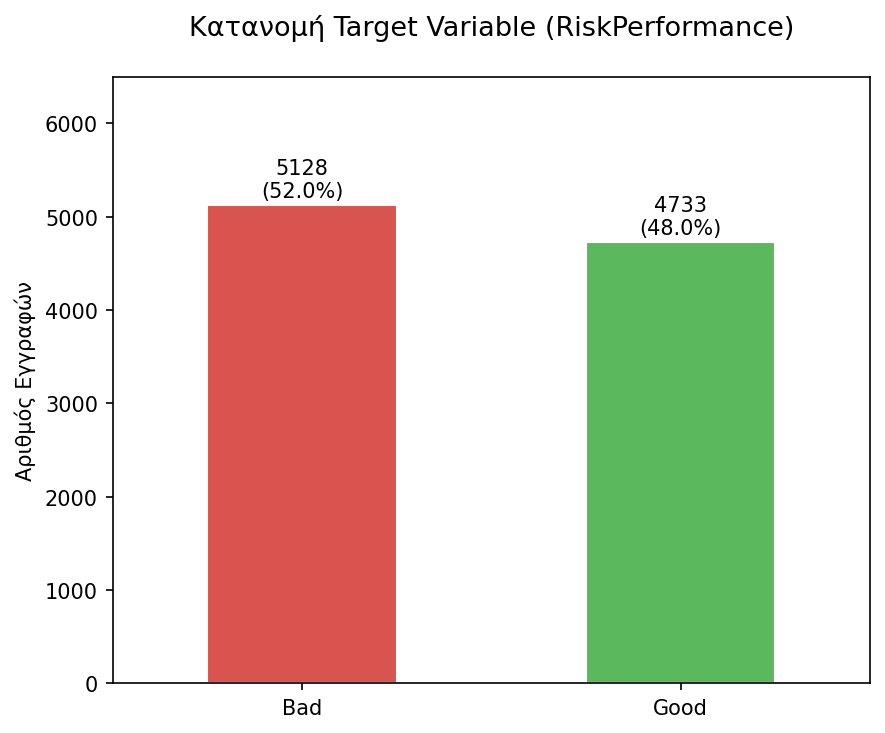
\includegraphics[width=0.55\textwidth]{01_target_distribution}
    \caption[Κατανομή μεταβλητής RiskPerformance]{Κατανομή της μεταβλητής \textit{RiskPerformance} μετά τον
             καθαρισμό της βάσης (9.861 εγγραφές). Η σχεδόν ισορροπημένη
             αναλογία Bad/Good δεν απαιτεί τεχνικές εξισορρόπησης κλάσεων.}
    \label{fig:target_dist}
\end{figure}

Τα αριθμητικά χαρακτηριστικά περιγράφουν το πιστωτικό ιστορικό του
κάθε δανειολήπτη. Ενδεικτικά, \textit{MSinceOldestTradeOpen} είναι οι
μήνες από την παλαιότερη πιστωτική συναλλαγή και
\textit{NetFractionRevolvingBurden} το ποσοστό χρήσης της διαθέσιμης
ανακυκλούμενης πίστωσης, όπως πιστωτικές κάρτες. Για παράδειγμα, σε
μια πιστωτική κάρτα με όριο τα 1.000 ευρώ, εάν έχει γίνει χρήση των
800 ευρώ, τότε το ποσοστό θα είναι 80\%. Όλα τα χαρακτηριστικά είναι
προϊόν επεξεργασίας της FICO με αποτέλεσμα οι σχέσεις μεταξύ τους να
είναι περισσότερο γραμμικές από το σύνηθες, γεγονός που τεκμηριώνεται
οπτικά στον πίνακα συσχέτισης του Σχήματος~\ref{fig:corr_matrix}. Το
γεγονός αυτό εξηγεί και τη μικρή διαφορά στην απόδοση μεταξύ της
Logistic Regression και των XGBoost, FFNN, όπως θα φανεί στο
Κεφάλαιο~\ref{ch:results}.

Ιδιαίτερο χαρακτηριστικό της βάσης αποτελεί η ύπαρξη τιμών $-9$, οι
οποίες συμβολίζουν την απουσία πληροφορίας. Συγκεκριμένα, 598 εγγραφές
αποτελούνται σχεδόν αποκλειστικά από τιμές $-9$, δηλαδή 598
δανειολήπτες δεν είχαν πιστωτικό ιστορικό. Παρά το ελλιπές ιστορικό,
στις εγγραφές αυτές υπάρχει \textit{RiskPerformance} (331 Bad, 267 Good),
αν και για λόγους που θα εξηγηθούν στην συνέχεια δεν θα
χρησιμοποιηθούν.

Η FICO HELOC είναι ευρέως εδραιωμένη στη βιβλιογραφία για την
ερμηνευσιμότητα της μηχανικής μάθησης, έτσι αποτελεί ιδανική επιλογή
για την παρούσα εργασία \citep{fico2018}. Τα δεδομένα της προέρχονται
από πραγματικές αιτήσεις και αποτελέσματα δανείων του τραπεζικού
συστήματος, γεγονός που προσδίδει πρακτικό χαρακτήρα στην παρούσα
εργασία.

\section{Προεπεξεργασία Δεδομένων}
\label{sec:preprocessing}
Όπως αναφέρθηκε και στην παράγραφο~\ref{sec:dataset} 598 εγγραφές από τις 10.459 
αποτελούνται σχεδόν αποκλειστικά από εγγραφές -9. Στην βάση μας αυτό σημαίνει 
απουσία πιστωτικού ιστορικού για τον υποψήφιο δανειολήπτη. Οι εγγραφές αυτές 
αφαιρέθηκαν από την βάση για δύο βασικούς λόγους. Πρώτον, δεν προσφέρουν κάποια 
πληροφορία από την οποία μπορεί να εκπαιδευτούν τα μοντέλα και δεύτερον το ποσοστό 
εμφάνισης τους είναι αρκετά μικρό ώστε η βάση να διατηρήσει την κλίμακα μεγέθους 
της και χωρίς αυτά. Η επιλογή listwise deletion έναντι imputation τεκμηριώνεται από τη βιβλιογραφία 
του missing data analysis, όπου σε περιπτώσεις που η έλλειψη πληροφορίας είναι 
συστηματική (Missing Not At Random) η εισαγωγή εκτιμώμενων τιμών εισάγει 
συστηματικό σφάλμα στις προβλέψεις \citep{little2019statistical, vanbuuren2018flexible}.
Ως τελικό αποτέλεσμα η βάση δεν περιέχει καμία εγγραφή -9. 
Η μόνη μη αριθμητική μεταβλητή RiskPerformance που έπαιρνε τιμές (\textit{Good}, 
\textit{Bad}) μετατράπηκε σε δυαδική χωρίς να χάνεται πληροφορία. Η αλλαγή αυτή 
είναι αναγκαία για την ορθή λειτουργία των μοντέλων ML. Το 0 πλέον αντιστοιχεί 
σε μη αθέτηση ενώ το 1 σε αθέτηση. Για την εκπαίδευση και αξιολόγηση των μοντέλων 
είναι γνωστό ότι χρειάζονται τρία διαφορετικά σύνολα δεδομένων. Αυτά τα σύνολα 
δημιουργήθηκαν από την επεξεργασμένη βάση FICO HELOC με την χρήση stratification 
(διαστρωμάτωση) ώστε η αναλογία 0/1 (\textit{Good}/\textit{Bad}) να είναι ίδια \citep{kohavi1995study}. 
Τα σύνολα training set (70\%) και validation set (15\%) χρησιμοποιούνται κατά την 
εκπαίδευση με το δεύτερο να έχει κύριο ρόλο στον έλεγχο για overfitting 
(υπερπροσαρμογή) και early stopping (πρόωρη διακοπή εκπαίδευσης). Το τελευταίο 
μέρος της βάσης test set (15\%) δεν εμφανίζεται κατά την εκπαίδευση αλλά γίνεται 
χρήση του κατά την τελική αξιολόγηση.

Για την ορθή χρήση των δεδομένων από τα ML μοντέλα είναι αναγκαίο αυτά να είναι 
όλα στην ίδια κλίμακα. Για να επιτευχθεί αυτό χωρίς την διαρροή πληροφορίας 
(data leakage)\citep{kaufman2012leakage, kapoor2023leakage} από το ένα set στο άλλο έγινε χρήση της τεχνικής StandardScaler 
με fit στο training set και transform σε validation και test sets. Αναλυτικά, fit 
είναι η διαδικασία μέσω της οποίας o αλγόριθμος μαθαίνει από τα δεδομένα και 
υπολογίζει μέση τιμή (mean) και τυπική απόκλιση (std) για κάθε δεδομένο, μια 
δυναμική δηλαδή διαδικασία, ενώ transform είναι η εφαρμογή των προηγούμενων 
ανεξάρτητα με τις τιμές των μεταβλητών. Πρακτικά αυτό διασφαλίζει ότι τα δεδομένα 
παραμένουν απομονωμένα και δεν είναι δυνατή η πρόβλεψη των υπόλοιπων συνόλων 
μέσω του training set. Η διαδικασία που περιγράφηκε γίνεται μια φορά στο πρώτο 
notebook του οποίου τα αποτελέσματα αποθηκεύονται σε αρχεία .npy, .pkl για να 
χρησιμοποιηθούν στο υπόλοιπο της εργασίας
(Σχήματα~\ref{fig:feature_dist_1} ,~\ref{fig:feature_dist_2} και~\ref{fig:corr_matrix}).

% -------------------------------------------------------------------
% Σχήμα 3.2 — Κατανομές 23 χαρακτηριστικών (NB01)
% Τοποθέτηση: τέλος ενότητας 3.2, μετά την αναφορά στα .npy/.pkl
% -------------------------------------------------------------------
\begin{figure}[!htbp]
    \centering
    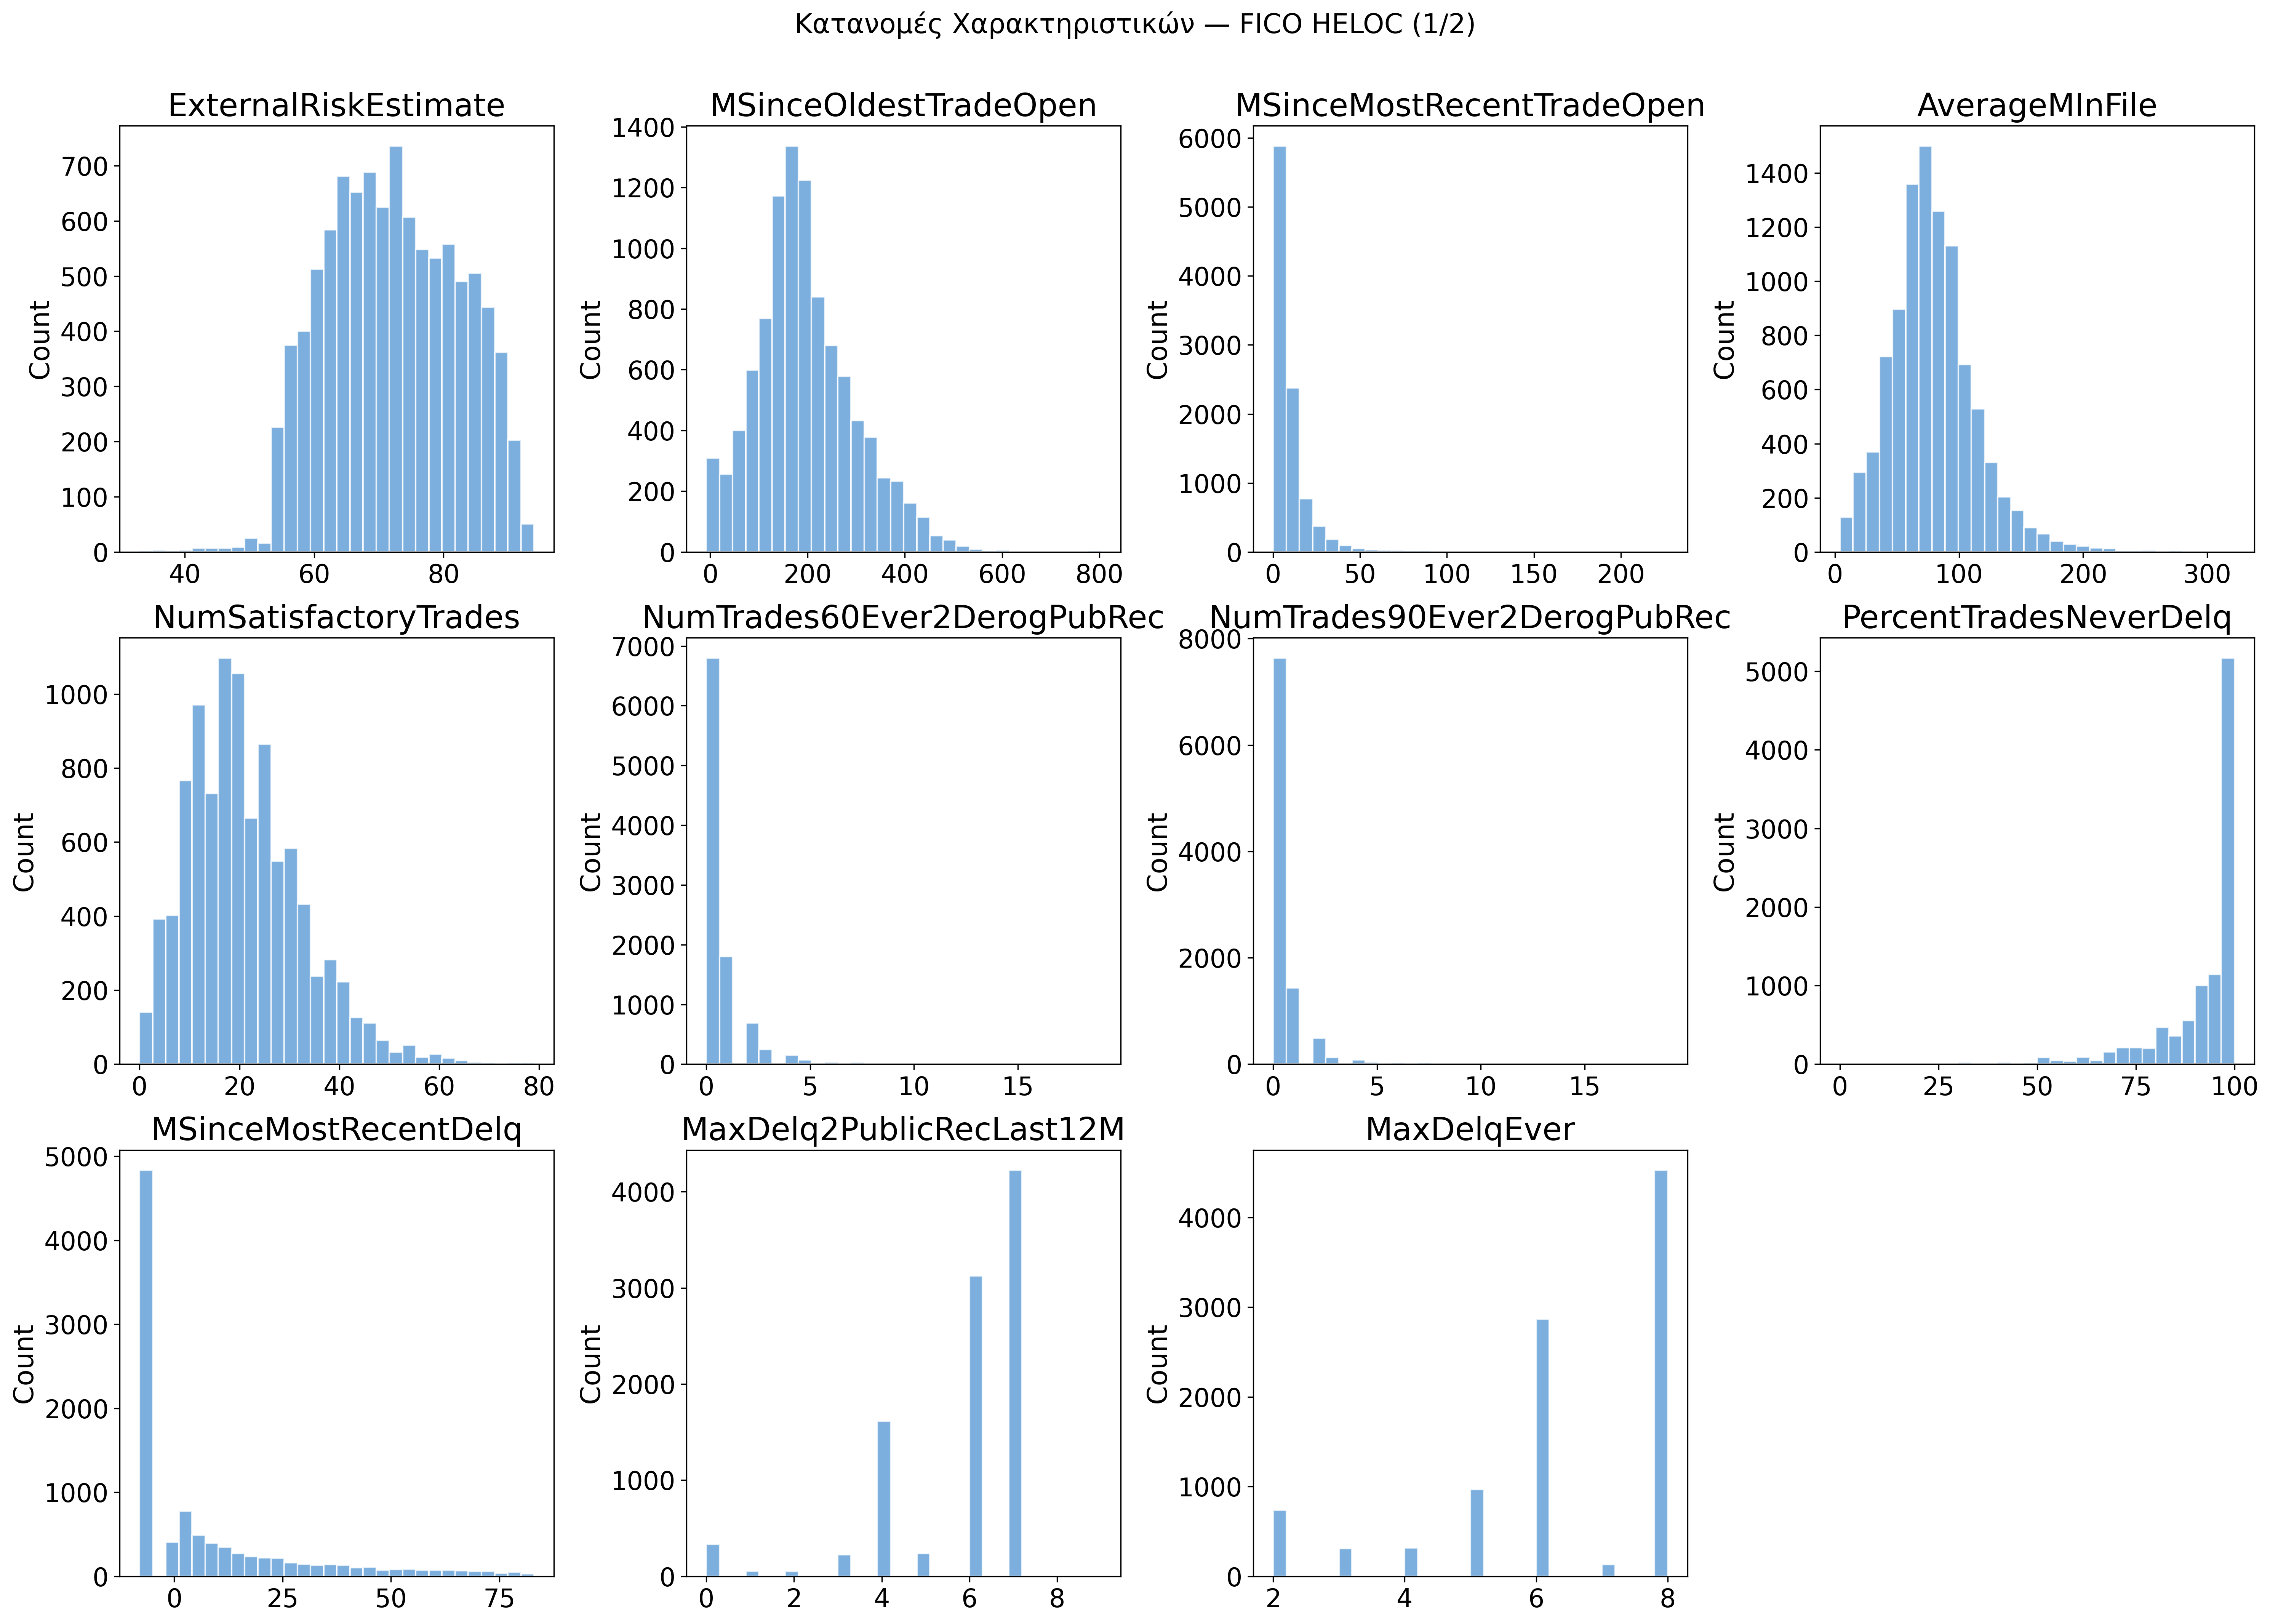
\includegraphics[width=\textwidth]{02_feature_distributions_part1}
    \caption[Κατανομές χαρακτηριστικών FICO HELOC (1/2)]{Κατανομές των πρώτων 11 χαρακτηριστικών της βάσης FICO HELOC μετά
             τον καθαρισμό. Παρατηρείται ποικιλία μορφών κατανομής
             (κανονική, ασύμμετρη, διακριτή) ανάλογα με τη φύση κάθε
             χαρακτηριστικού (1/2).}
    \label{fig:feature_dist_1}
\end{figure}

\begin{figure}[!htbp]
    \centering
    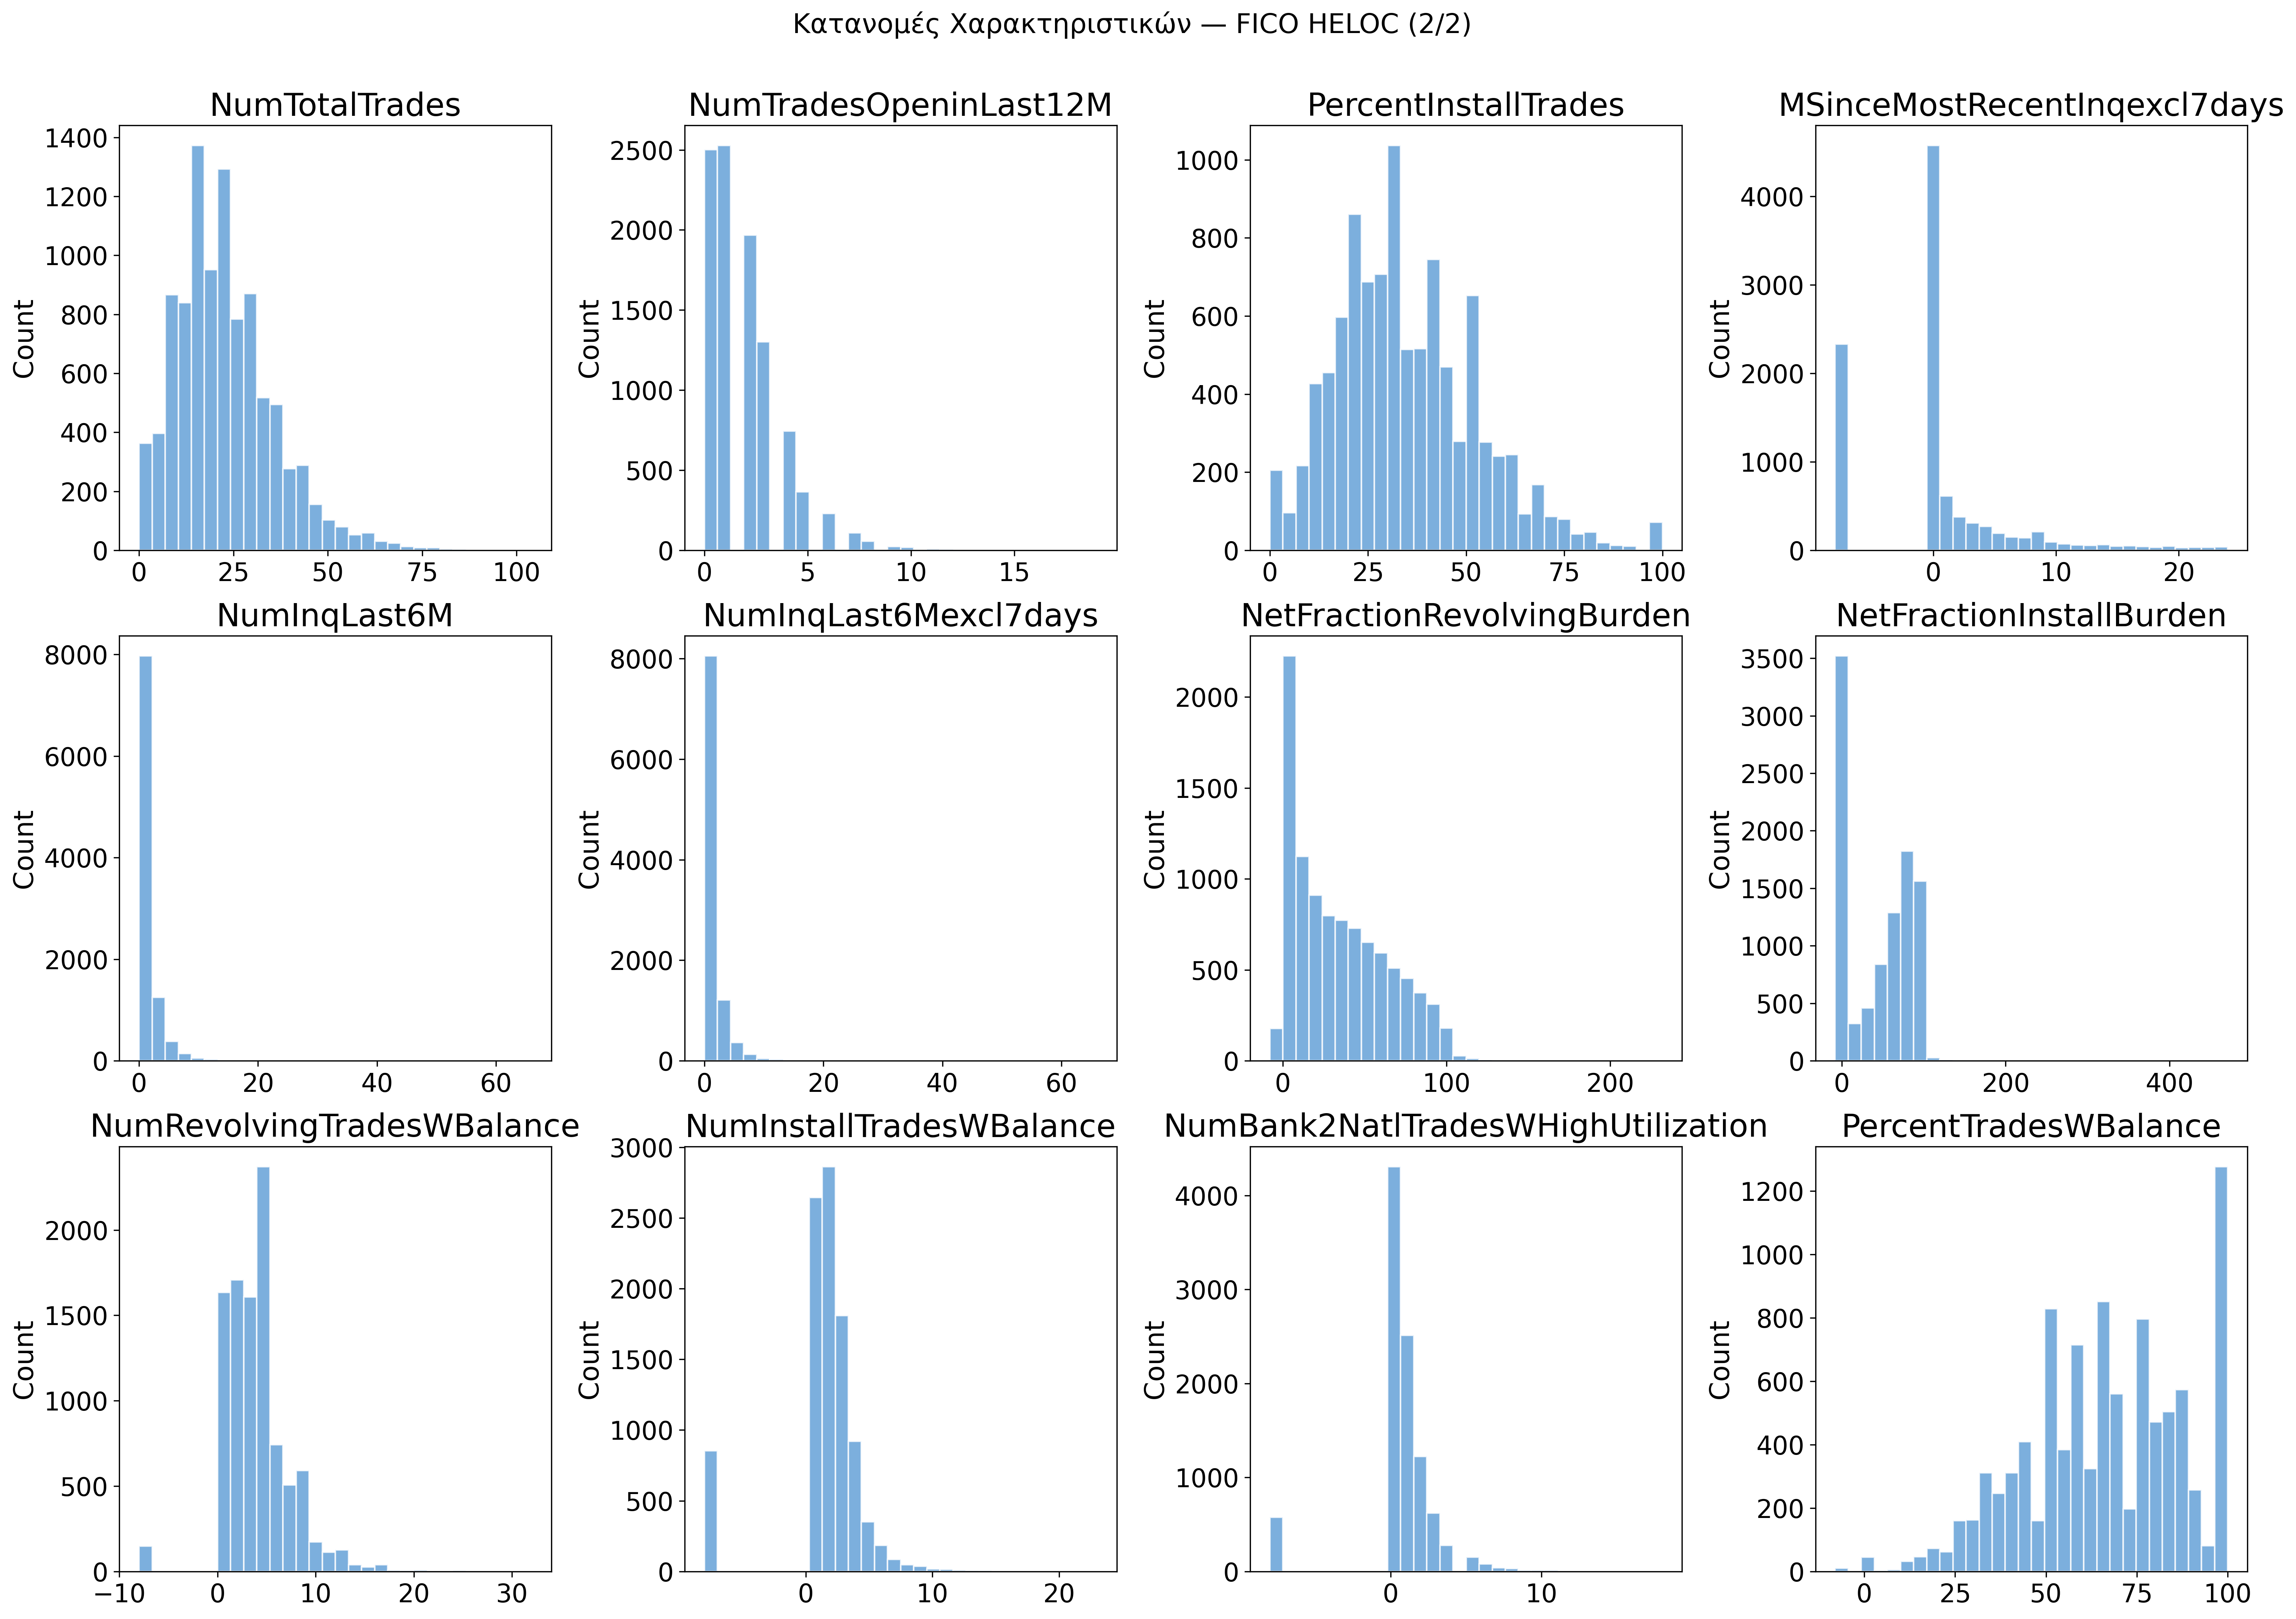
\includegraphics[width=\textwidth]{02_feature_distributions_part2}
    \caption[Κατανομές χαρακτηριστικών FICO HELOC (2/2)]{Κατανομές των υπόλοιπων 12 χαρακτηριστικών της βάσης FICO HELOC μετά
             τον καθαρισμό (2/2).}
    \label{fig:feature_dist_2}
\end{figure}

% -------------------------------------------------------------------
% Σχήμα 3.3 — Πίνακας συσχέτισης (NB01)
% Τοποθέτηση: αμέσως μετά το Σχήμα 3.2 — τα δύο σχήματα
% προεπεξεργασίας παραμένουν μαζί στο τέλος της ενότητας
% -------------------------------------------------------------------
\begin{figure}[!htbp]
    \centering
    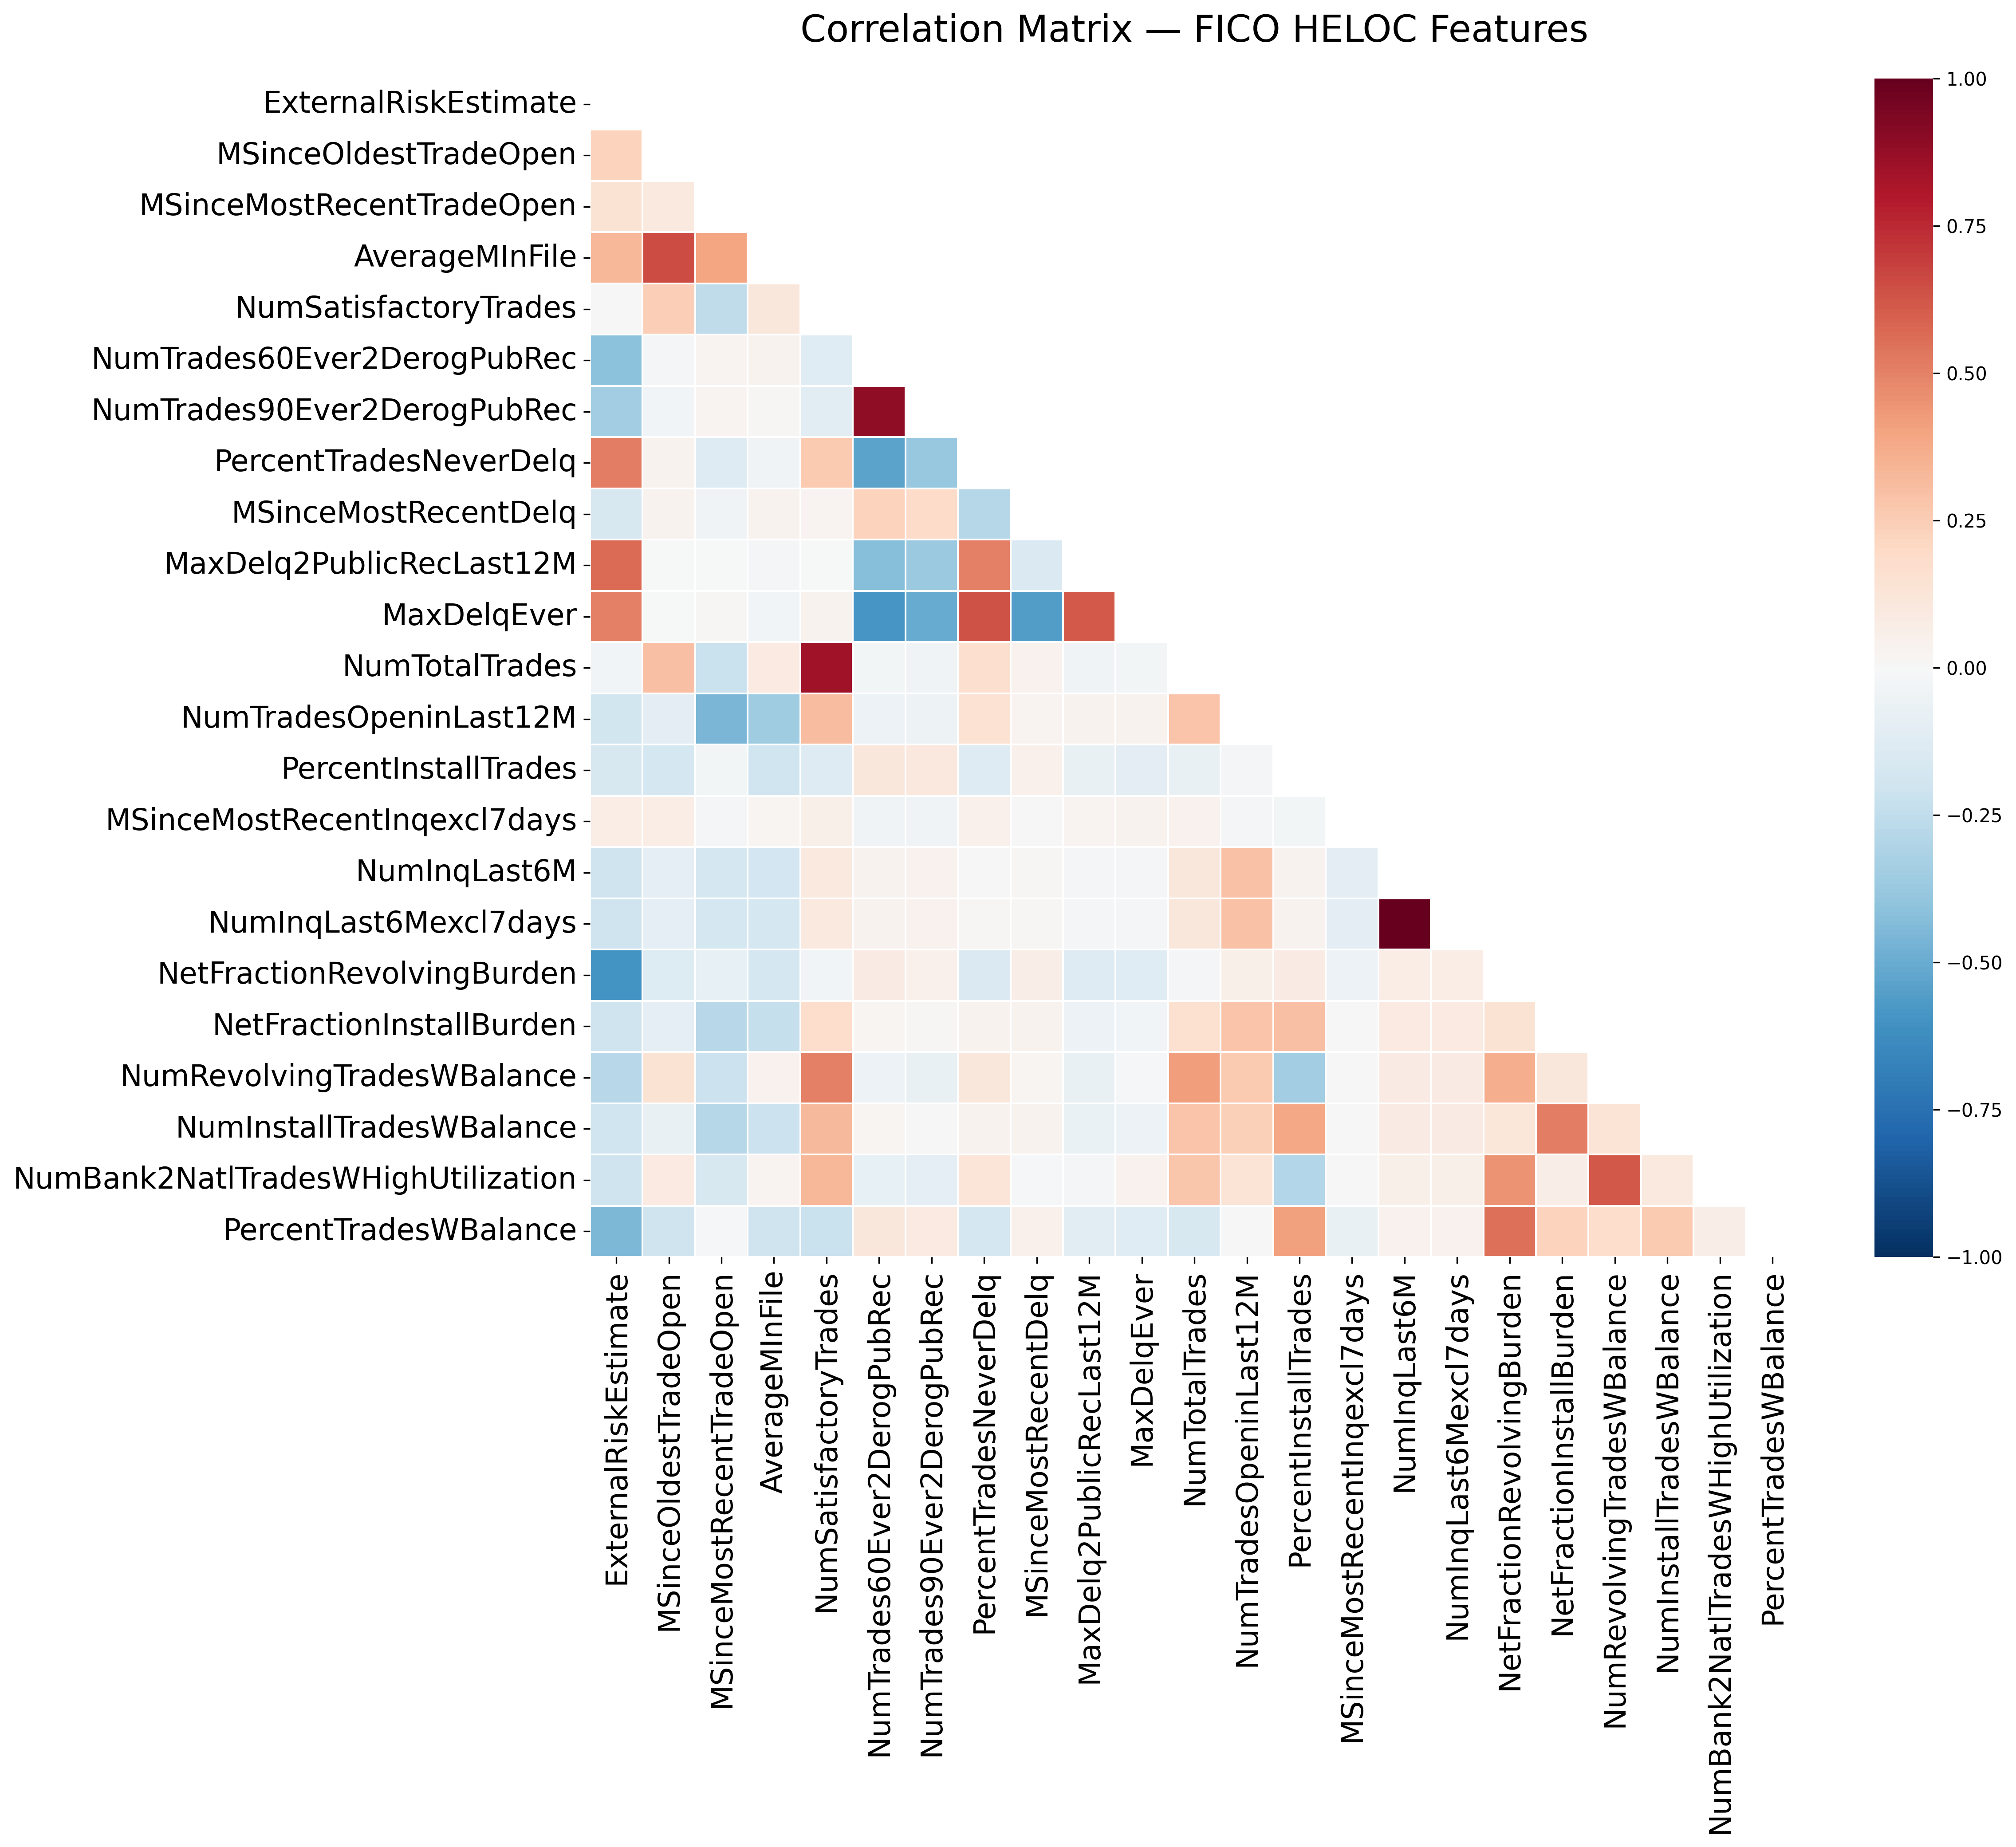
\includegraphics[width=\textwidth]{03_correlation_matrix}
    \caption[Πίνακας συσχέτισης χαρακτηριστικών FICO HELOC]{Πίνακας συσχέτισης (lower triangle) των 23 χαρακτηριστικών
             της βάσης FICO HELOC. Η αυξημένη γραμμικότητα μεταξύ των
             χαρακτηριστικών αποτελεί συνέπεια της επεξεργασίας δεδομένων
             από την FICO και εξηγεί εν μέρει τη μικρή διαφορά απόδοσης
             μεταξύ των μοντέλων.}
    \label{fig:corr_matrix}
\end{figure}

\section{Μοντέλα}
\label{sec:models}

\subsection{Logistic Regression}
\label{sec:lr}
Η πιο διαδεδομένη υλοποίηση της Logistic Regression είναι αυτή της βιβλιοθήκης 
scikit-learn σε γλώσσα Python οπότε επιλέχθηκε για την εργασία. Έγινε εφαρμογή 
της με όλες τις default (προεπιλεγμένες) επιλογές παραμέτρων αλλά η σύγκλιση 
δεν ήταν ικανοποιητική. Για τον λόγο αυτό εκπαιδεύτηκε με \texttt{max\_iter=1000} 
αντί 100. Σε κάθε ερευνητική εργασία είναι απαραίτητη η ύπαρξη ενός στόχου, 
ορίου το οποίο να κάνει την αξιολόγηση των αποτελεσμάτων προφανή. Αυτός είναι 
ο ρόλος της LR. Αποτελεί το κύριο μοντέλο στον τραπεζικό τομέα με την πλήρη 
αποδοχή των εποπτικών αρχών λόγω της πλήρους ερμηνευσιμότητάς της, άρα η χρήση 
κάποιου άλλου μοντέλου δικαιολογείται μόνο εάν αυτό χαρακτηρίζεται από καλύτερη 
απόδοση. Τα υπόλοιπα μοντέλα λοιπόν πρέπει να αποδείξουν ότι μπορούν να κάνουν 
καλύτερες προβλέψεις, να περάσουν δηλαδή το όριο που θέτει η LR για να 
δικαιολογηθούν οι επιπλέον δυσκολίες απόρροια της πολυπλοκότητάς τους.


\subsection{XGBoost}
\label{sec:xgboost}

Το μοντέλο XGBoost με το πλήρες όνομα eXtreme Gradient Boosting ανήκει στην
οικογένεια αλγορίθμων τεχνητής νοημοσύνης που χρησιμοποιούν δέντρα αποφάσεων.
Συγκεκριμένα, είναι υλοποίηση του αλγορίθμου Gradient Boosting. Στην πράξη, το
μοντέλο κατά την εκπαίδευσή του φτιάχνει πολλαπλά δέντρα αποφάσεων μικρού βάθους,
τα οποία χρησιμοποιεί στη συνέχεια για να κάνει προβλέψεις. Η δενδρική του αυτή
δομή είναι και ο λόγος που έγινε η επιλογή χρήσης μη κανονικοποιημένων
χαρακτηριστικών (raw features) αντί κλιμακωμένων (scaled), 
καθώς τα δέντρα αποφάσεων είναι αναλλοίωτα ως προς μονότονους μετασχηματισμούς 
των χαρακτηριστικών \citep{hastie2009}. Οι παράμετροι
εκπαίδευσης παρουσιάζονται στον Πίνακα~\ref{tab:xgb_params} ομαδοποιημένοι σε
τρεις κατηγορίες. Αποφεύχθηκε η βελτιστοποίηση υπερπαραμέτρων (hyperparameter
tuning) και οι παράμετροι επιλέχθηκαν ως λογικές αρχικές τιμές που αποφεύγουν
το overfitting \citep{probst2019tunability, bentejac2021comparative}. 
Οι βασικοί λόγοι επιλογής του XGBoost είναι η κυρίαρχη θέση του
στη βιβλιογραφία και η ικανότητα ερμηνευσιμότητάς του μέσω του TreeExplainer του
SHAP \citep{chen2016xgboost}. Όσον αφορά τα μοντέλα μηχανικής μάθησης στον
πιστωτικό κίνδυνο, η υλοποίηση XGBoost χαίρει ευρείας αποδοχής τόσο στην
αποδοτικότητα όσο και στην επικύρωση και παρακολούθησή του. Την ίδια αποδοχή και
αξιοπιστία χαίρει και το TreeExplainer, το οποίο χρησιμοποιείται για να εξηγήσει
τη συμπεριφορά παρόμοιων μοντέλων, και εφόσον είναι συμβατό με το XGBoost,
αποτελεί έναν επιπλέον λόγο επιλογής του. Ως κύριο μοντέλο της εργασίας, πάνω
του θα πραγματοποιηθούν πλήρης ανάλυση SHAP, ανίχνευση μεροληψίας (bias
detection) και παρακολούθηση (monitoring), ενώ η σύγκριση με τη Logistic
Regression θα αποκαλύψει τι επιπλέον απαιτήσεις επιφέρει η αυξημένη πολυπλοκότητα
και πώς αυτές μπορούν να ικανοποιηθούν.

\begin{table}[htbp]
\centering
\caption{Παράμετροι εκπαίδευσης XGBoost}
\label{tab:xgb_params}
\begin{tabular}{llp{7cm}}
\toprule
\textbf{Κατηγορία} & \textbf{Παράμετρος} & \textbf{Τιμή \& Αιτιολόγηση} \\
\midrule
\multirow{3}{*}{Δομή \& Εκπαίδευση}
  & \texttt{n\_estimators} & 300 — αρκετά δέντρα για ακρίβεια χωρίς υπερβολικό υπολογιστικό κόστος \\
  & \texttt{max\_depth}    & 4 — περιορισμός βάθους για αποφυγή overfitting \\
  & \texttt{learning\_rate}& 0.05 — μικρό βήμα μάθησης, συνδυάζεται με τα 300 δέντρα \\
\midrule
\multirow{2}{*}{Τυχαιοποίηση}
  & \texttt{subsample}        & 0.8 — κάθε δέντρο εκπαιδεύεται σε τυχαίο 80\% των εγγραφών \\
  & \texttt{colsample\_bytree}& 0.8 — κάθε δέντρο χρησιμοποιεί τυχαίο 80\% των χαρακτηριστικών \\
\midrule
\multirow{3}{*}{Τεχνικές}
  & \texttt{eval\_metric}        & auc — κατάλληλο για δυαδική ταξινόμηση \\
  & \texttt{random\_state}       & 42 — αναπαραγωγιμότητα αποτελεσμάτων \\
  & \texttt{early\_stopping\_rounds}& 20 - διακοπή εκπαίδευσης εάν η απόδοση στο validation set δεν βελτιωθεί για 20 συνεχόμενους γύρους, αποτρέποντας την υπερπροσαρμογή\\ 
\bottomrule
\end{tabular}
\end{table}

\subsection{Feed-Forward Neural Network}
\label{sec:ffnn}

Μια διαφορετική κατηγορία μοντέλων μηχανικής μάθησης είναι τα νευρωνικά δίκτυα \citep{goodfellow2016deep}.
Στην κατηγορία αυτή ανήκει το μοντέλο FFNN (Feed Forward Neural Network) με την
ιδιαιτερότητα ότι η πληροφορία σε αυτό κινείται μόνο προς μια κατεύθυνση, από
την είσοδο στα κρυφά επίπεδα (hidden layers) και τέλος στην έξοδο. Αναλυτικά
στην εργασία το μοντέλο έχει δύο hidden layers όπου σε κάθε ένα μειώνονται οι
νευρώνες, από 64 σε 32. Η επιλογή αυτή έγινε λόγω του πλήθους των features,
23 σε αριθμό, και έχοντας ως στόχο την αποφυγή της υπερσυμπίεσης της πληροφορίας
μέσω απότομης μείωσης των νευρώνων. Κάθε νευρώνας έχει και ένα βάρος με το οποίο
φιλτράρει την πληροφορία σε μη δυαδική μορφή και με όρια διαφορετικά του $(0,1)$,
για τον λόγο αυτό στην έξοδο εφαρμόζεται μια sigmoid activation συνάρτηση που
μετατρέπει την πληροφορία σε πιθανότητα ανάμεσα σε 0 και 1, μορφή κατάλληλη για
την εργασία μετά την εφαρμογή ορίου μετατροπής (threshold). Κάθε νευρώνας έχει
δύο καταστάσεις «ενεργοποιημένος» και «μη ενεργοποιημένος». Η συνάρτηση που
αποφασίζει για την κατάσταση αυτή είναι η ReLU activation \citep{glorot2011deep} η οποία επιστρέφει
μηδέν σε αρνητικές τιμές «μη ενεργοποίηση» και τις τιμές ατόφιες για θετικές
για κατάσταση «ενεργοποίησης». Για την εκπαίδευσή του το μοντέλο απαιτεί
κανονικοποιημένα δεδομένα, οπότε σε αντίθεση με το XGBoost έγινε επεξεργασία
των δεδομένων με προσοχή στο data leakage όπως αναφέρθηκε στην
ενότητα~\ref{sec:preprocessing}. Επιπλέον, για την αποφυγή overfitting στα
δεδομένα ορίστηκε Dropout=0.3/0.2 \citep{srivastava2014dropout} το οποίο απενεργοποιεί τυχαία 30\% των νευρώνων
έτσι ώστε το μοντέλο να βασίζεται σε όλους τους νευρώνες του σχεδόν ισότιμα.
Η μεταβλητή Epochs=100 με EarlyStopping(patience=15) \citep{prechelt1998early} ορίζει το πόσες φορές θα
εκπαιδευτεί το μοντέλο στα δεδομένα με όριο τις 100 φορές, εκτός εάν σε 10
συνεχόμενες εποχές δεν βελτιωθεί το αποτέλεσμά του. Η μεταβλητή αυτή είναι
σημαντική γιατί επιτρέπει να μην οριστεί ακριβές όριο μετεκπαίδευσης που θα
μπορούσε να οδηγήσει σε χειρότερο αποτέλεσμα αλλά και υπερεκπαίδευση. Οι
υπόλοιπες τεχνικές παράμετροι εκπαίδευσης παρουσιάζονται συνοπτικά στον
Πίνακα~\ref{tab:ffnn_params}. Τα δεδομένα της HELOC λόγω της επεξεργασίας που
έχει γίνει από την FICO έχουν αυξημένη γραμμικότητα μεταξύ τους. Για τον λόγο
αυτό οι διαφορές ανάμεσα στην απόδοση των μοντέλων θα είναι μειωμένες, γεγονός
που δεν αποτελεί μειονέκτημα για την εργασία καθώς ο σκοπός είναι η σύγκριση
των μοντέλων ως προς τις ανάγκες παρακολούθησης και ερμηνείας τους. Η σύγκριση
της FFNN με τα υπόλοιπα μοντέλα θα γίνει κυρίως πάνω σε αυτό τον σκοπό.

\begin{table}[htbp]
\centering
\caption{Παράμετροι εκπαίδευσης Feed-Forward Neural Network}
\label{tab:ffnn_params}
\begin{tabular}{llp{7cm}}
\toprule
\textbf{Κατηγορία} & \textbf{Παράμετρος} & \textbf{Τιμή \& Αιτιολόγηση} \\
\midrule
\multirow{2}{*}{Βελτιστοποίηση}
  & \texttt{optimizer}      & Adam \citep{kingma2015adam} --- προσαρμοστικός αλγόριθμος, standard επιλογή για FFNN \\
  & \texttt{learning\_rate} & 0.001 --- προεπιλογή Adam, σταθερή σύγκλιση \\
\midrule
Συνάρτηση κόστους
  & \texttt{loss}           & binary crossentropy --- θεωρητικά ορθή για δυαδική ταξινόμηση \citep{goodfellow2016deep} \\
\midrule
Εκπαίδευση
  & \texttt{batch\_size}    & 64  --- ισορροπία ταχύτητας και σταθερότητας εκπαίδευσης \\
\bottomrule
\end{tabular}
\end{table}

\section{Μεθοδολογία Επικύρωσης}
\label{sec:val_methodology}

\subsection{Αξιολόγηση Απόδοσης}
\label{sec:performance}
Τα μοντέλα αφού εκπαιδευτήκαν στο train και validation δοκιμάστηκαν στο test set.
Για την αξιολόγηση των μοντέλων χρησιμοποιήθηκε πλήθος δεικτών που αποτελούν 
standard στον τομέα του credit scoring \citep{hand1997statistical, anderson2007credit}.


\paragraph{AUC-ROC \& Gini.}
Ο δείκτης AUC-ROC μετράει το εμβαδόν κάτω από την καμπύλη ROC και αποτελεί τον
σημαντικότερο δείκτη όσων αφορά τον πιστωτικό κίνδυνο \citep{hand2009measuring}. Η καμπύλη ROC σχηματίζεται
στον άξονα True Positive Rate (ποσοστό Bad που εντοπίστηκαν σωστά) και False
Positive Rate (ποσοστό Good που κατατάχθηκαν λανθασμένα ως Bad) και το εμβαδόν
μετράει την ικανότητα του μοντέλου να κάνει σωστές προβλέψεις σε κάθε threshold,
δηλαδή σε κάθε όριο πιθανότητας πάνω από το οποίο η πρόβλεψη μετατρέπεται σε Bad.
Η AUC-ROC παίρνει τιμές κοντά στο 0,5 για μοντέλα χωρίς προβλεπτική ικανότητα
και έτσι τα αποτελέσματα των ικανών για προβλέψεις μοντέλων συνήθως κυμαίνονται
στο πεδίο $(0{,}5,\ 1)$. Για πιο ξεκάθαρα αποτελέσματα στην κλίμακα $(0,1)$
χρησιμοποιείται ο δείκτης Gini ο οποίος προκύπτει από την σχέση $2 \times
\text{AUC} - 1$.

\paragraph{KS (Kolmogorov-Smirnov).}
Ενώ οι προηγούμενοι δείκτες φανερώνουν την απόδοση ανεξάρτητα από threshold,
ο KS εντοπίζει σε ποια τιμή του το μοντέλο έχει την βέλτιστη απόδοση. Για να
το πετύχει αυτό δημιουργεί μια φθίνουσα λίστα επικινδυνότητας και δύο αθροιστικές
κατανομές. Οι κατανομές οπτικοποιούνται ως καμπύλες και φανερώνουν το ποσοστό
Bad και Good μέχρι κάθε συγκεκριμένο σημείο της λίστας. Το σημείο στο οποίο οι
καμπύλες διαφέρουν το μέγιστο είναι το κατάλληλο threshold.

\paragraph{Πίνακας Σύγχυσης \& Ανάλυση Ορίου Απόφασης.}
Επειδή το κόστος κάθε Ψευδώς Θετικού (False Positive) δεν είναι πάντα ίδιο
με το κόστος ενός Ψευδώς Αρνητικού (False Negative) χρειάζονται και άλλες μετρικές
όπως ο Πίνακας Σύγχυσης (Confusion Matrix). Για συγκεκριμένο threshold (0.5 στην
παρούσα εργασία) ο Πίνακας Σύγχυσης είναι ένας $2\times2$ πίνακας με το σύνολο
των TP (True Positive), TN (True Negative), FP (False Positive) και FN (False
Negative). Στον πιστωτικό κίνδυνο η ελαχιστοποίηση του FN, των δανειοληπτών που
δεν θα μπορέσουν να πληρώσουν το δάνειο, είναι απαραίτητη. Συμπληρωματικά
λειτουργεί η Ανάλυση Ορίου Απόφασης (Threshold Analysis). Το Threshold Analysis
αποτελείται από γραφήματα τριών μετρικών, της Precision, Recall και F1 οι οποίες
υπολογίζονται για κάθε threshold. Η Precision υπολογίζει από τους προβλεπόμενους
Bad πόσοι ήταν πραγματικά Bad, η Recall υπολογίζει από τους πραγματικούς Bad
πόσους εντόπισε το μοντέλο, ενώ η F1 είναι ο αρμονικός μέσος των προηγούμενων
δύο.

\paragraph{Ανάλυση Κατά Δεκατημόρια (Decile Analysis).}
Κλασική μετρική στον οικονομικό τομέα, χωρίζει το δείγμα ανάλογα με την
προβλεπόμενη επικινδυνότητα σε 10 ομάδες και ελέγχει το ποσοστό προβλέψεων Bad
(Bad Rate) σε αυτές. Ένα καλό προβλεπτικό μοντέλο αναμένεται να έχει μεγάλο
Bad Rate στα πρώτα Decile ενώ μικρότερο στα επόμενα. Στην εργασία χρησιμοποιείται
επίσης το Αθροιστικό Ποσοστό Αθέτησης (Cumulative Bad Rate) στο οποίο φαίνεται
το αθροιστικό ποσοστό των Bad ανά δεκατημόριο και συγκρίνεται με την διαγώνιο
που αντιστοιχεί σε μοντέλο χωρίς προβλεπτική ικανότητα.

\paragraph{Βαθμονόμηση (Calibration).}
Η Βαθμονόμηση εξετάζει κατά πόσο οι προβλεπόμενες πιθανότητες αθέτησης
αντιστοιχούν στα πραγματικά δεδομένα. Η μέτρηση αυτή είναι αναγκαία στον
πιστωτικό κίνδυνο. Οι κανόνες της Basel III επιβάλλουν την ακριβή τιμολόγηση
επιτοκίων και τον υπολογισμό αποθεματικών κεφαλαίου τα οποία βασίζονται στις
προβλέψεις των ποσοστών αθέτησης \citep{basel2017}. Για να κρίνουμε πόσο ακριβές είναι αυτό το
ποσοστό, ομαδοποιούμε τους δανειολήπτες με βάση αυτή την πιθανότητα και για
κάθε ομάδα (bin) της μορφής $(x,\ x+\Delta y)\%$ βρίσκουμε την πραγματική
πιθανότητα αθέτησης. Έτσι στο Calibration Plot ένα μοντέλο με τέλεια ικανότητα
βαθμονόμησης θα ακολουθεί την διαγώνιο εφόσον η ομαδοποίηση θα ταυτίζεται με
τα πραγματικά αποτελέσματα. Ο στόχος των μοντέλων είναι να πλησιάζουν όσο
περισσότερο την διαγώνιο. Η μετρική αυτή διαφέρει από την AUC καθώς η δεύτερη
αρκείται στην ταξινόμηση των δανειοληπτών και όχι στην ακριβή πρόβλεψη του
ποσοστού αθέτησης.

\subsection{Ανίχνευση Μεροληψίας}
\label{sec:bias_methodology}

Η Ανίχνευση Μεροληψίας (Bias Detection) ελέγχει εάν οι προβλέψεις του μοντέλου
χειρίζονται κάθε υποομάδα με τον ίδιο τρόπο. Ο διαχωρισμός των ομάδων γίνεται
συνήθως με βάση το φύλο, ηλικία ή εθνικότητα του δανειολήπτη. Στην παρούσα
εργασία επειδή η βάση δεν περιέχει προσωπικά δεδομένα οι ομάδες χωρίζονται με
βάση την μεταβλητή \texttt{AverageMInFile}. Η χρήση proxy μεταβλητής αποτελεί καθιερωμένη πρακτική στη βιβλιογραφία fairness 
όταν τα προστατευόμενα χαρακτηριστικά δεν είναι διαθέσιμα στη βάση δεδομένων 
\citep{chen2019fairness}, και επιτρέπει την εμπειρική επίδειξη της μεθοδολογίας 
ανίχνευσης μεροληψίας χωρίς να αντικαθιστά την ανάλυση σε πραγματικά 
δημογραφικά χαρακτηριστικά. Η ομάδα Α με
\texttt{AverageMInFile} κάτω της διαμέσου έχει μικρότερο πιστωτικό
παρελθόν ενώ η Β με τιμές πάνω της διαμέσου μεγαλύτερο. Η σύγκριση των ποσοστών
έγκρισης κάθε ομάδας είναι η κύρια διαφορά με την AUC και Calibration οι οποίες
κάνουν μόνο ατομικούς ελέγχους σε κάθε δανειολήπτη. Οι δύο κυριότερες μετρικές
της Bias Detection είναι η Δημογραφική Ισότητα (Demographic Parity) και η
Ανισομερής Επίπτωση (Disparate Impact). Στην DPD (Demographic Parity Difference)
γίνεται σύγκριση του ποσοστού έγκρισης των δύο ομάδων με αποδεκτό όριο το
$0{,}1$. Στην DI (Disparate Impact Ratio) υπολογίζεται ο λόγος των ποσοστών
έγκρισης και το όριο είναι το $0{,}8$. Οι δύο αυτές μετρικές είναι
συμπληρωματικές και δίνουν διαφορετικές πληροφορίες. Στην εργασία παρατηρείται
bias, δηλαδή οι τιμές ξεπερνούν τα όρια που αναφέρθηκαν, οπότε εφαρμόζονται δύο τεχνικές μετριασμού που ανήκουν στην καθιερωμένη ταξονομία 
pre/in/post-processing \citep{kamiran2012data}: \texttt{ExponentiatedGradient} 
\citep{agarwal2018reductions} με περιορισμό Demographic Parity για την Logistic 
Regression (in-processing) και χειροκίνητος ThresholdOptimizer \citep{hardt2016equality} 
μέσω grid search για το XGBoost (post-processing).
Και οι δύο τεχνικές προσαρμόζουν τα όρια απόφασης ξεχωριστά για κάθε ομάδα.
Με τον τρόπο αυτό τα μοντέλα έχουν αποδεκτή, μικρότερη μεροληψία αλλά η
απόδοσή τους επηρεάζεται --- για την Logistic Regression μειώνεται το AUC,
ενώ για το XGBoost το AUC παραμένει αμετάβλητο και μειώνεται το Balanced
Accuracy. Το αποτέλεσμα αυτό είναι αναμενόμενο καθώς η διαδικασία στοχεύει
στην διατήρηση μικρής διαφοράς ανάμεσα στα ποσοστά έγκρισης για κάθε ομάδα
και όχι στην καλύτερη δυνατή πρόβλεψη για κάθε δανειολήπτη ξεχωριστά.

\subsection{Σταθερότητα Πληθυσμού (PSI)}
\label{sec:psi}

Η Σταθερότητα Πληθυσμού (PSI) υπολογίζει εάν τα δεδομένα εκπαίδευσης
αποκλίνουν από τα δεδομένα πρόβλεψης της τρέχουσας χρονικής περιόδου.
Η μετρική αυτή στοχεύει στην ανίχνευση αλλαγών στα δεδομένα εισόδου
και όχι στην αξιολόγηση της ποιότητας των προβλέψεων. Στην πράξη
χωρίζει τις προβλεπόμενες πιθανότητες σε δέκα ομάδες με ίσα διαστήματα
από μηδέν μέχρι ένα. Έπειτα για κάθε ομάδα υπολογίζεται το ποσοστό
εγγραφών για τα δύο σύνολα (reference dataset και current dataset).
Τέλος με τον μαθηματικό τύπο:
\begin{equation}
    PSI = \sum_{i=1}^{n} (A_i - E_i) \times \ln\left(\frac{A_i}{E_i}\right)
    \label{eq:psi}
\end{equation}
υπολογίζεται ο δείκτης PSI, όπου $A_i$ είναι το ποσοστό εγγραφών στο
current dataset και $E_i$ στο reference dataset για κάθε ομάδα $i$.
Εάν ο δείκτης είναι μικρότερος του $0{,}10$ έχουμε σταθερή κατανομή,
εάν είναι ανάμεσα σε $0{,}10$ και $0{,}25$ υπάρχει μέτρια μετατόπιση
στα δεδομένα και η παρακολούθηση κρίνεται αναγκαία, ενώ για τιμές
μεγαλύτερες του $0{,}25$ απαιτείται επανεκπαίδευση του μοντέλου.
Στην εργασία τα δεδομένα της βάσης προέρχονται από μια συγκεκριμένη
χρονική περίοδο οπότε έγινε προσομοίωση μελλοντικών δεδομένων με την
χρήση Γκαουσιανού θορύβου. Έγινε η υπόθεση ότι η μελλοντική οικονομία
θα υποστεί μια ύφεση με τους βασικούς δείκτες να αλλάζουν.
Συγκεκριμένα, οι δείκτες \texttt{ExternalRiskEstimate} και
\texttt{AverageMInFile} μειώθηκαν διότι κατά την διάρκεια μιας
οικονομικής ύφεσης το πιστωτικό προφίλ χειροτερεύει και το πιστωτικό
ιστορικό ελαττώνεται, ενώ αυξάνεται το χρέος και κατά συνέπεια ο
δείκτης \texttt{NetFractionRevolvingBurden}. Έγινε προσομοίωση τριών εντάσεων, ήπιας, μέτριας και σοβαρής επιδείνωσης
με κλιμακώμενη ένταση θορύβου ανάλογα με τη σοβαρότητα. Με τον τρόπο αυτό γίνεται
ευδιάκριτη η χρησιμότητα της μετρικής.

\section{Εξειδικευμένη Ανάλυση XGBoost}
\label{sec:xgboost_analysis}

Τα μοντέλα τεχνητής νοημοσύνης συνήθως παράγουν καλύτερα αποτελέσματα στον
πιστωτικό κίνδυνο εισάγοντας όμως παράλληλα και έναν συμβιβασμό (trade-off).
Όσο πιο περίπλοκα είναι τόσο λιγότερο ερμηνεύσιμη είναι η διαδικασία που
ακολούθησαν για να εξάγουν το αποτέλεσμα. Το μοντέλο XGBoost είναι το κύριο
μοντέλο της εργασίας αλλά και το κυρίαρχο μοντέλο στον τομέα του διότι
βρίσκεται στο σημείο της χρυσής τομής του trade-off. Το XGBoost προσφέρει
αισθητή βελτίωση αποδοτικότητας έναντι της Logistic Regression, διατηρώντας
παράλληλα επαρκή ερμηνευσιμότητα για την ανάλυση που ακολουθεί. Σε αυτή την
ενότητα θα γίνει ανάλυση των μετρικών και δεικτών που εξηγούν τους λόγους για
τους οποίους το μοντέλο πήρε τις συγκεκριμένες αποφάσεις αλλά και των τεχνικών
παρακολούθησης των μοντέλων μετά το τέλος της εκπαίδευσής τους. Οι μετρήσεις
αυτές δεν αποτελούν αυτοσκοπό αλλά είναι αναγκαίες καθώς αποτελούν
προαπαιτούμενο από τις διάφορες ρυθμιστικές αρχές (Basel, EBA) \citep{basel2017, eba2023}.

\subsection{Ερμηνευσιμότητα --- SHAP}
\label{sec:shap}

Για να εξηγήσουμε μια απόφαση έγκρισης δανείου δεν αρκεί ένα ποσοστό.
Η χρήση εργαλείων που εξηγούν την πιθανότητα αθέτησης και κατά συνέπεια
την απόφαση έγκρισης ή μη του δανείου είναι αναγκαία. Το SHAP (SHapley
Additive exPlanations) μέσω της θεωρίας Shapley values του τομέα της
θεωρίας παιγνίων καταφέρνει να αποκωδικοποιήσει τη συμπεριφορά του
μοντέλου. Μέσω του SHAP μπορούμε να καταλάβουμε κατά πόσο επηρέασε η
κάθε μεταβλητή το αποτέλεσμα. Η λειτουργία του είναι διπλή, διακρίνεται
στην ολική ανάλυση των δεδομένων (Global SHAP) και στην ατομική ανάλυση
(Local SHAP).Οι τιμές αυτές είναι αθροιστικές: το άθροισμά τους μαζί με
την τιμή αναφοράς (base value) ισούται με την τελική πρόβλεψη του μοντέλου
για τον συγκεκριμένο δανειολήπτη.
Το Local SHAP υπολογίζει για κάθε χαρακτηριστικό του
δανειολήπτη μια τιμή SHAP που συμβολίζει τη συνεισφορά του στην τελική
πρόβλεψη. Από τις τιμές αυτές γίνεται δυνατή η ικανοποίηση του
«δικαιώματος εξήγησης» του αιτούντος πελάτη. Το Global SHAP υπολογίζει
τη μέση απόλυτη τιμή από κάθε SHAP τιμή και παράγει πιο γενικά
αποτελέσματα που εξηγούν τη λειτουργία του μοντέλου. Από τα αποτελέσματα
γίνονται σαφή τα χαρακτηριστικά τα οποία αυτό θεωρεί σημαντικότερα.

Η λειτουργία του PDP (Partial Dependence Plots) είναι συμπληρωματική του SHAP.
Ενώ το SHAP απαντάει στο πόσο επηρεάζει κάθε χαρακτηριστικό, το PDP
συμπληρώνει τον τρόπο με τον οποίο το κάνει. Για κάθε χαρακτηριστικό
δοκιμάζει πολλαπλές τιμές του σε όλους τους υποψήφιους δανειολήπτες και
καταγράφει τις αλλαγές στην τελική πρόβλεψη. Ως αποτέλεσμα, παράγονται
διαγράμματα που παρουσιάζουν τη μη γραμμική συσχέτιση των χαρακτηριστικών
με τον υπολογισμό του ποσοστού αθέτησης. Η μη γραμμική ``σκέψη'' του
μοντέλου είναι αυτή που το ξεχωρίζει από την Logistic Regression.

\subsection{Σταθερότητα Χαρακτηριστικών (CSI)}
\label{sec:csi}

Ο δείκτης CSI (Characteristic Stability Index) λειτουργεί συμπληρωματικά
του PSI. Χρησιμοποιεί τον ίδιο μαθηματικό τύπο (βλ.\ εξίσωση~\ref{eq:psi})
για κάθε χαρακτηριστικό αντί μόνο του μεμονωμένου ποσοστού πρόβλεψης.
Οι τιμές CSI κάτω του $0{,}10$ μεταφράζονται ως σταθερό χαρακτηριστικό,
οι τιμές μεταξύ $0{,}10$ και $0{,}25$ ως ύπαρξη μέτριας μετατόπισης,
ενώ για τιμές άνω του $0{,}25$ ύπαρξη σημαντικής αστάθειας. Σημαντική
πληροφορία αποτελεί ότι ο δείκτης CSI βασίζεται σε ιστόγραμμα (histogram)
οπότε είναι ιδιαίτερα ευαίσθητος όταν αξιολογεί διακριτές τιμές. Ακόμα
και μικρές μεταβολές των διακριτών τιμών μπορούν να προκαλέσουν τεχνητά
υψηλές τιμές του δείκτη. Στην εργασία η χρησιμότητα αυτού του δείκτη
θα φανεί μέσω του τροποποιημένου dataset.


\subsection{Παρακολούθηση Μοντέλου}
\label{sec:monitoring_methodology}

Έπειτα από το πέρας της εκπαίδευσης, της επικύρωσης και των τελικών
ελέγχων η τελευταία ασπίδα προστασίας για τη διαφύλαξη της σωστής
λειτουργίας του μοντέλου είναι η παρακολούθηση μοντέλου (Monitoring).
Η φθορά απόδοσης του μοντέλου με το χρόνο (Model Drift) είναι
αναμενόμενη. Για τον λόγο αυτό ο συνεχής έλεγχος είναι προαπαιτούμενο
και βασική απαίτηση των εποπτικών αρχών \citep{eba2023}. Η παρακολούθηση μοντέλου
εστιάζει στους δείκτες PSI --- παρακολουθεί αλλαγές στα ποσοστά των
προβλέψεων --- CSI --- παρακολουθεί αλλαγές στα ποσοστά των
χαρακτηριστικών --- και AUC over time --- παρακολουθεί την προβλεπτική
ικανότητα του μοντέλου. Στην παρούσα εργασία ο έλεγχος γίνεται σε
δεδομένα που προσομοιώνουν ήπια, μέτρια και σοβαρή οικονομική
επιδείνωση για τα μοντέλα XGBoost και FFNN. Η βασική διαφορά των
μοντέλων κατά την διαδικασία βρίσκεται στην ανάγκη χρήσης της
συνάρτησης KernelExplainer \citep{lundberg2017shap} 
αντί της TreeExplainer \citep{lundberg2020local} για το μοντέλο FFNN,
η οποία αναμένεται να αυξήσει σημαντικά την πολυπλοκότητα και ως
απόρροια τις ώρες υπολογισμού.   % Δεδομένα, Μοντέλα & Μεθοδολογία
%==============================================================
% ΚΕΦΑΛΑΙΟ 4 — ΠΕΙΡΑΜΑΤΙΚΑ ΑΠΟΤΕΛΕΣΜΑΤΑ
%==============================================================
\chapter{Πειραματικά Αποτελέσματα}
\label{ch:results}

Στο παρόν κεφάλαιο παρουσιάζονται τα αποτελέσματα που προκύπτουν
από τα δεδομένα, τα μοντέλα και τις μεθοδολογίες που περιεγράφηκαν
αναλυτικά στο Κεφάλαιο~\ref{ch:methodology}.
Τα αποτελέσματα εστιάζουν στους τέσσερις άξονες: απόδοση,
ερμηνευσιμότητα, μεροληψία και παρακολούθηση.
Η σειρά παρουσίασης τους είναι ίδια με αυτή της μεθοδολογίας.
Το κύριο μοντέλο της εργασίας είναι το XGBoost, ενώ παράλληλα
δοκιμάζονται και τα μοντέλα Logistic Regression ως βασικό εργαλείο
του πιστωτικού κίνδυνου, αλλά και το FFNN ως πολυπλοκότερο μοντέλο
τεχνητής νοημοσύνης.
Για κάθε αποτέλεσμα υπάρχει και ένα τουλάχιστον γράφημα που βοηθάει
στην οπτικοποίηση του, ενώ παράλληλα παρέχεται ανάλυση ως προς
την σημαντικότητα και ερμηνεία του.
Κεντρικό εύρημα του κεφαλαίου αποτελεί η μη γραμμική σχέση ανάμεσα
στην πολυπλοκότητα, την απόδοση και τις απαιτήσεις επικύρωσης.
Οι τρεις αυτοί άξονες έχουν αυξημένη βαρύτητα στην επιλογή μοντέλου
στον πιστωτικό κίνδυνο, γεγονός που δίνει πρακτική χρησιμότητα
στα ευρήματα.

%--------------------------------------------------------------
\section{Αξιολόγηση Απόδοσης Μοντέλων}
\label{sec:performance_results}

\subsection{Μετρικές Αξιολόγησης}
\label{subsec:metrics}
Η εκπαίδευση των μοντέλων έγινε με τις παραμέτρους που
περιγράφηκαν αναλυτικά στο Κεφάλαιο~\ref{ch:methodology}.
Η αξιολόγηση έγινε επάνω στο test set, μέρος της βάσης
HELOC που προέκυψε από την διαίρεση της.
Τα παρακάτω διαγράμματα των μετρικών AUC-ROC, Gini και
KS statistic αποκαλύπτουν την πλήρη εικόνα
όσον αφορά τον πρώτο άξονα αξιολόγησης τους, την απόδοση.
Για κάθε μετρική τα αποτελέσματα παρουσιάζονται με πλήρη
ανάλυση στη συνέχεια.



\subsection{Σύγκριση Μοντέλων και Κατανομή Σκορ}
\label{subsec:model_comparison}

Η παρούσα υποενότητα περιέχει την ανάλυση και τις τιμές
των μετρικών που αναφέρθηκαν στην
υποενότητα~\ref{subsec:metrics}.
Ο Πίνακας~\ref{tab:model_metrics} συνοψίζει τις τιμές
των AUC, Gini και KS για τα μοντέλα Logistic Regression,
XGBoost και FFNN.

\begin{table}[htbp]
    \centering
    \caption[Σύγκριση μετρικών απόδοσης — test set]{Σύγκριση μετρικών απόδοσης στο test set.
    Με έντονη γραφή η καλύτερη τιμή ανά μετρική.}
    \label{tab:model_metrics}
    \begin{tabular}{lccc}
        \toprule
        \textbf{Μοντέλο} & \textbf{AUC} & \textbf{Gini} & \textbf{KS} \\
        \midrule
        Logistic Regression & 0.789          & 0.579          & 0.455 \\
        XGBoost             & \textbf{0.796} & \textbf{0.593} & 0.458 \\
        FFNN                & 0.793          & 0.587          & \textbf{0.465} \\
        \bottomrule
    \end{tabular}
\end{table}


% -------------------------------------------------------------------
% 04_model_comparison.png
% Επεξήγηση ευρημάτων της 04_model_comparison.png
% -------------------------------------------------------------------

Όπως φαίνεται στο Σχήμα~\ref{fig:model_comparison},
στις μετρικές AUC-ROC (0{,}796) και Gini (0{,}593)
το μοντέλο XGBoost υπερτερεί έναντι των Logistic
Regression (0{,}789, 0{,}579) και του FFNN (0{,}793,
0{,}587).
Στη μετρική KS το μοντέλο FFNN (0{,}465) έχει ελαφρώς
καλύτερη απόδοση από το XGBoost (0{,}458) και
Logistic Regression (0{,}455).
Οι διαφορές μεταξύ των μοντέλων και στους τρεις
δείκτες είναι οριακές, οπότε δεν συνιστούν πραγματική
διαφορά στην απόδοση και αποτελεσματικότητα αυτών.
Οι μικρές αυτές διαφορές ήταν αναμενόμενες, καθώς
οφείλονται στη γραμμικότητα της βάσης FICO HELOC
όπως αναφέρθηκε στην ενότητα~\ref{sec:dataset}.
Το παρόν εύρημα υποστηρίζει την υπόθεση ότι η απόδοση
δεν είναι ανάλογη της πολυπλοκότητας του μοντέλου.

% -------------------------------------------------------------------
% 04_model_comparison.png
% Σχήμα 4.1 — Grouped bar chart σύγκρισης μοντέλων (NB02)
% Τοποθέτηση: αμέσως μετά τον Πίνακα 4.1
% -------------------------------------------------------------------
\begin{figure}[htbp]
    \centering
    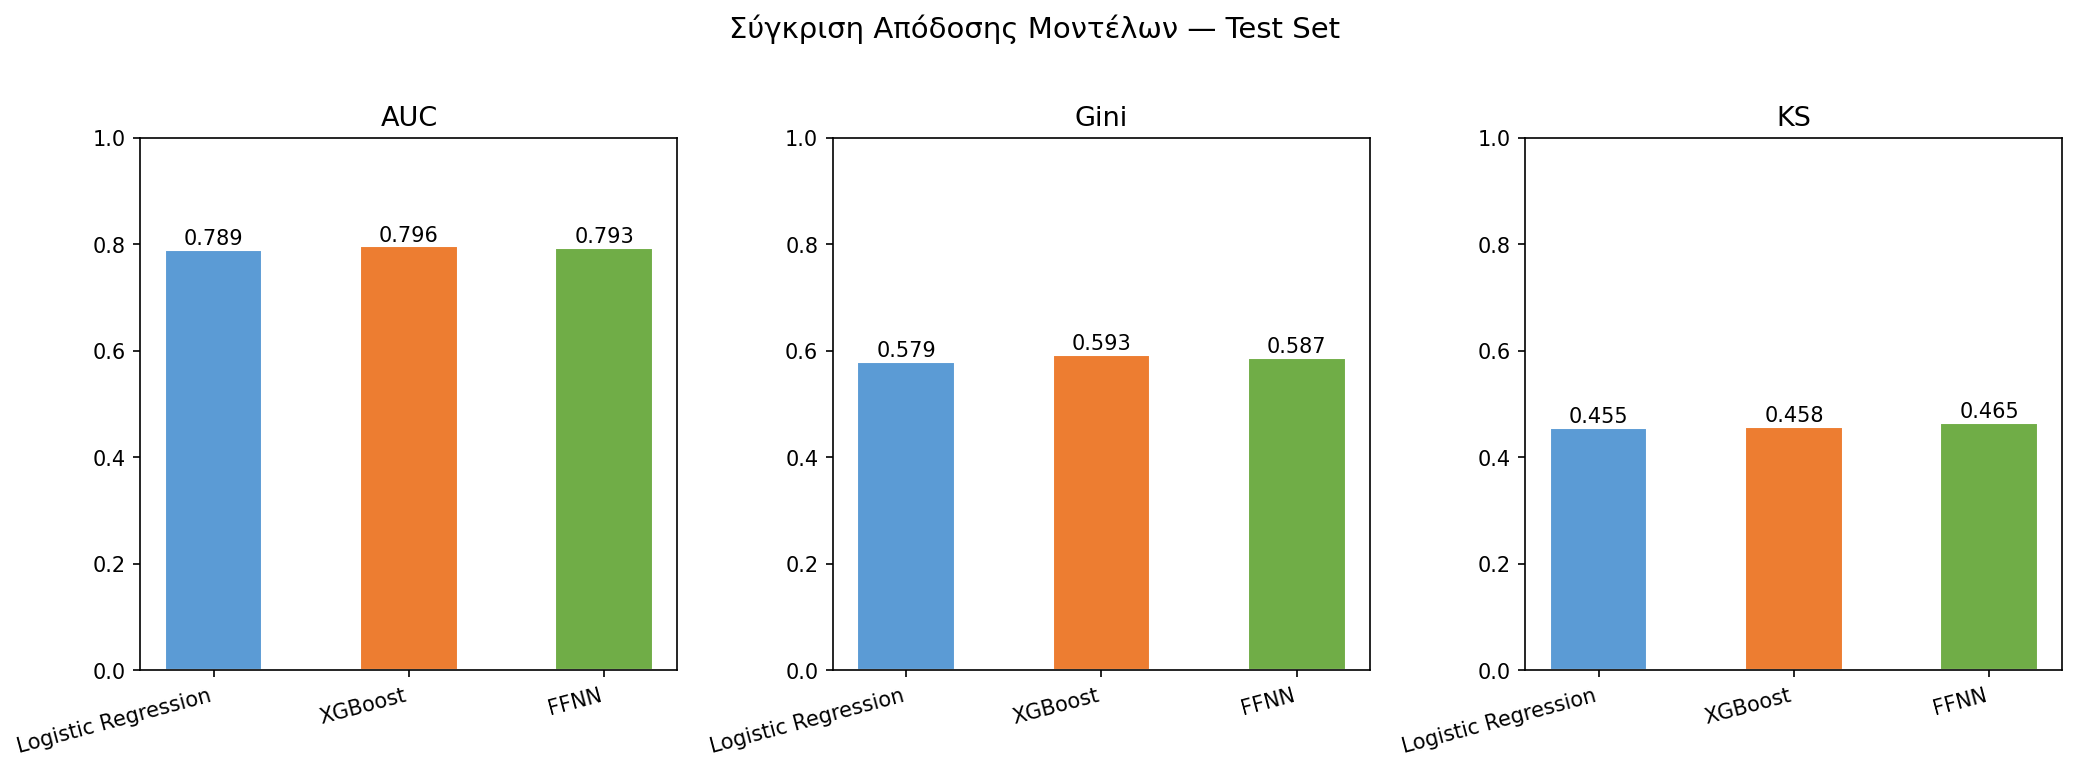
\includegraphics[width=\textwidth]{04_model_comparison}
    \caption[Σύγκριση μοντέλων — AUC, Gini, KS]{Σύγκριση των τριών μοντέλων στο test set για τους δείκτες AUC-ROC,
             Gini και KS. Οι μικρές διαφορές αποδόσεως αναδεικνύουν ότι η
             αυξημένη πολυπλοκότητα δεν συνεπάγεται ανάλογη βελτίωση.}
    \label{fig:model_comparison}
\end{figure}

\subsection{Καμπύλες ROC}
\label{sec:roc}

Το Σχήμα~\ref{fig:roc_curves} παρουσιάζει τις καμπύλες ROC και των τριών μοντέλων
μαζί με τη διαγώνιο τυχαίας βασικής γραμμής (AUC = 0{,}500). Και τα τρία μοντέλα
βρίσκονται σαφώς πάνω από τη διαγώνιο, επιβεβαιώνοντας την προβλεπτική τους
ικανότητα. Η οπτική απόσταση μεταξύ τους είναι πολύ μικρή, συνεπής με τα
αριθμητικά αποτελέσματα του Πίνακα~\ref{tab:model_metrics}. Η καμπύλη ROC
είναι ανεξάρτητη από το επιλεγμένο threshold, άρα δεν επηρεάζεται από την
επιχειρηματική απόφαση για το όριο αποδοχής δανείου. Αυτό την καθιστά ιδανική
μετρική για τη σύγκριση της ικανότητας διαχωρισμού μεταξύ μοντέλων.

% -------------------------------------------------------------------
% Σχήμα 4.2 — ROC Curves (NB02)
% Τοποθέτηση: αμέσως μετά τον έλεγχο καμπυλών ROC
% -------------------------------------------------------------------
\begin{figure}[htbp]
    \centering
    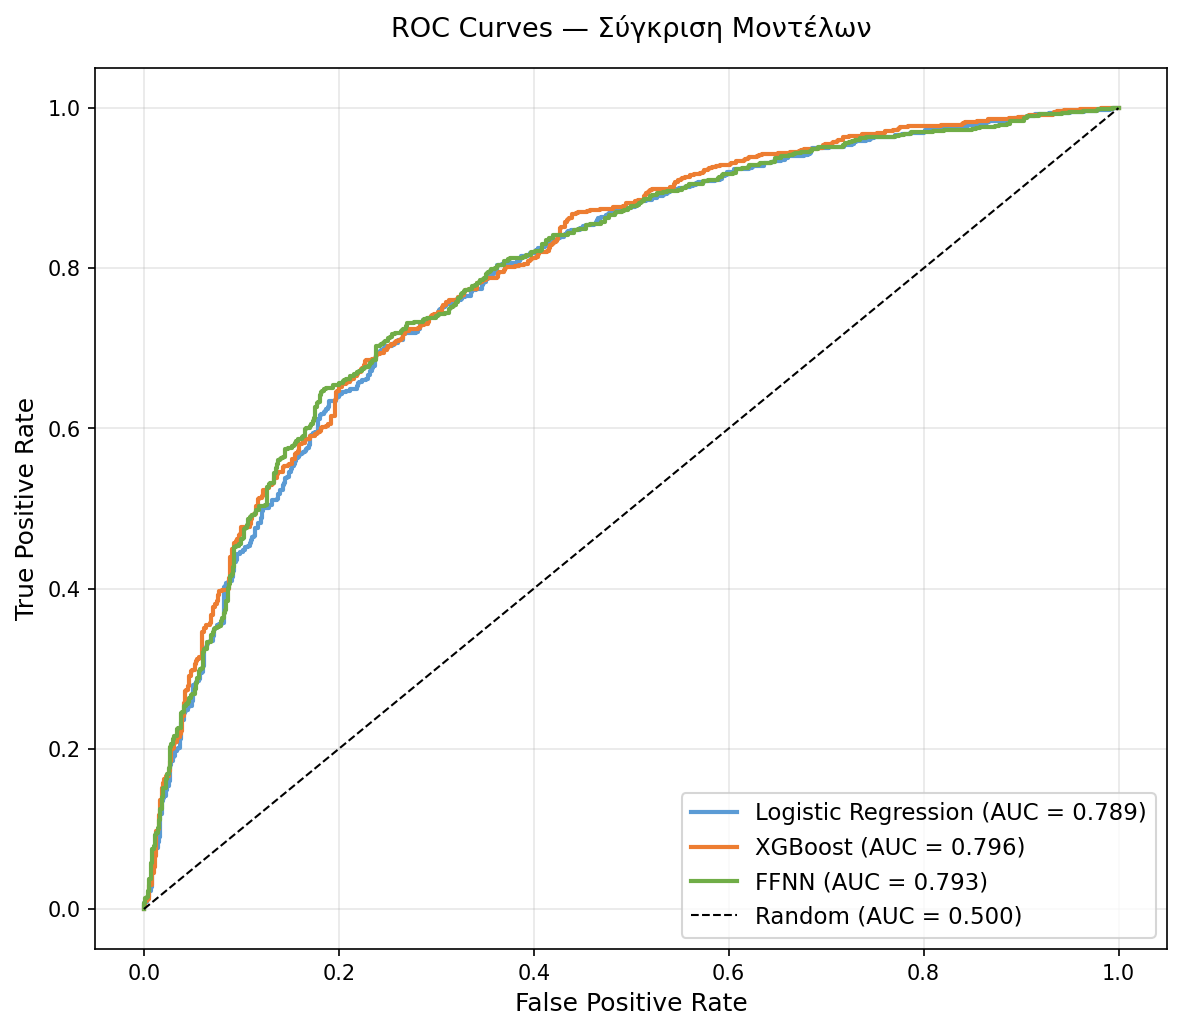
\includegraphics[width=0.80\textwidth]{14_roc_curves}
    \caption[Καμπύλες ROC τριών μοντέλων]{Καμπύλες ROC και των τριών μοντέλων στο test set. Η διαγώνιος
             αντιστοιχεί σε τυχαίο μοντέλο χωρίς προβλεπτική ικανότητα
             (AUC = 0{,}500). Η μικρή οπτική απόσταση μεταξύ των καμπυλών
             αντικατοπτρίζει τις μικρές διαφορές απόδοσης.}
    \label{fig:roc_curves}
\end{figure}



% 16_score_distribution.png
Τα τρία διαφορετικά overlapping histograms στο
Σχήμα~\ref{fig:score_distribution} οπτικοποιούν την πιθανοτική
κατανομή των δανειοληπτών για κάθε μοντέλο.
Οι δανειολήπτες με δάνειο που κατέληξε σε αθέτηση
συμβολίζονται με κόκκινο ενώ οι υπόλοιποι με πράσινο.
Ένα μοντέλο με τέλεια προβλεπτική ικανότητα θα παρήγε
διάγραμμα με τις δύο κατανομές συγκεντρωμένες στο 0 (Good)
και 1 (Bad).
Τα αποτελέσματα της εργασίας διαφέρουν από μια τέτοια
κατανομή καθώς παρατηρούνται περιπτώσεις Good και Bad
σε όλο σχεδόν το φάσμα, γεγονός αναμενόμενο για πραγματικά
δεδομένα που εισάγουν τυχαιότητα.
Είναι εμφανής και στα τρία διαγράμματα η τάση των μοντέλων
να τοποθετούν τις τιμές Good κοντά στο 0 και Bad κοντά στο 1.
Αυτή η συμπεριφορά υποδηλώνει προβλεπτική ικανότητα και
συμφωνεί με τα αποτελέσματα των προηγούμενων σχημάτων.
Τέλος, υπάρχει επικάλυψη κατανομών η οποία υποδηλώνει
αβεβαιότητα των μοντέλων ως προς την ταξινόμηση η οποία
όμως είναι ελεγχόμενη και αναμενόμενη σε μη ιδανικά μοντέλα.
Η παρατηρούμενη επικάλυψη είναι συνεπής με τις οριακές
διαφορές AUC και Gini του Πίνακα~\ref{tab:model_metrics},
επιβεβαιώνοντας ότι και οι τρεις μέθοδοι αξιολόγησης ---
πίνακας μετρικών, καμπύλες ROC και κατανομή σκορ ---
οδηγούν στο ίδιο συμπέρασμα.

% -------------------------------------------------------------------
% Σχήμα 4.3 — Κατανομή σκορ Bad/Good ανά μοντέλο (NB03)
% Τοποθέτηση: αμέσως μετά το κείμενο ανάλυσης
% -------------------------------------------------------------------
\begin{figure}[htbp]
    \centering
    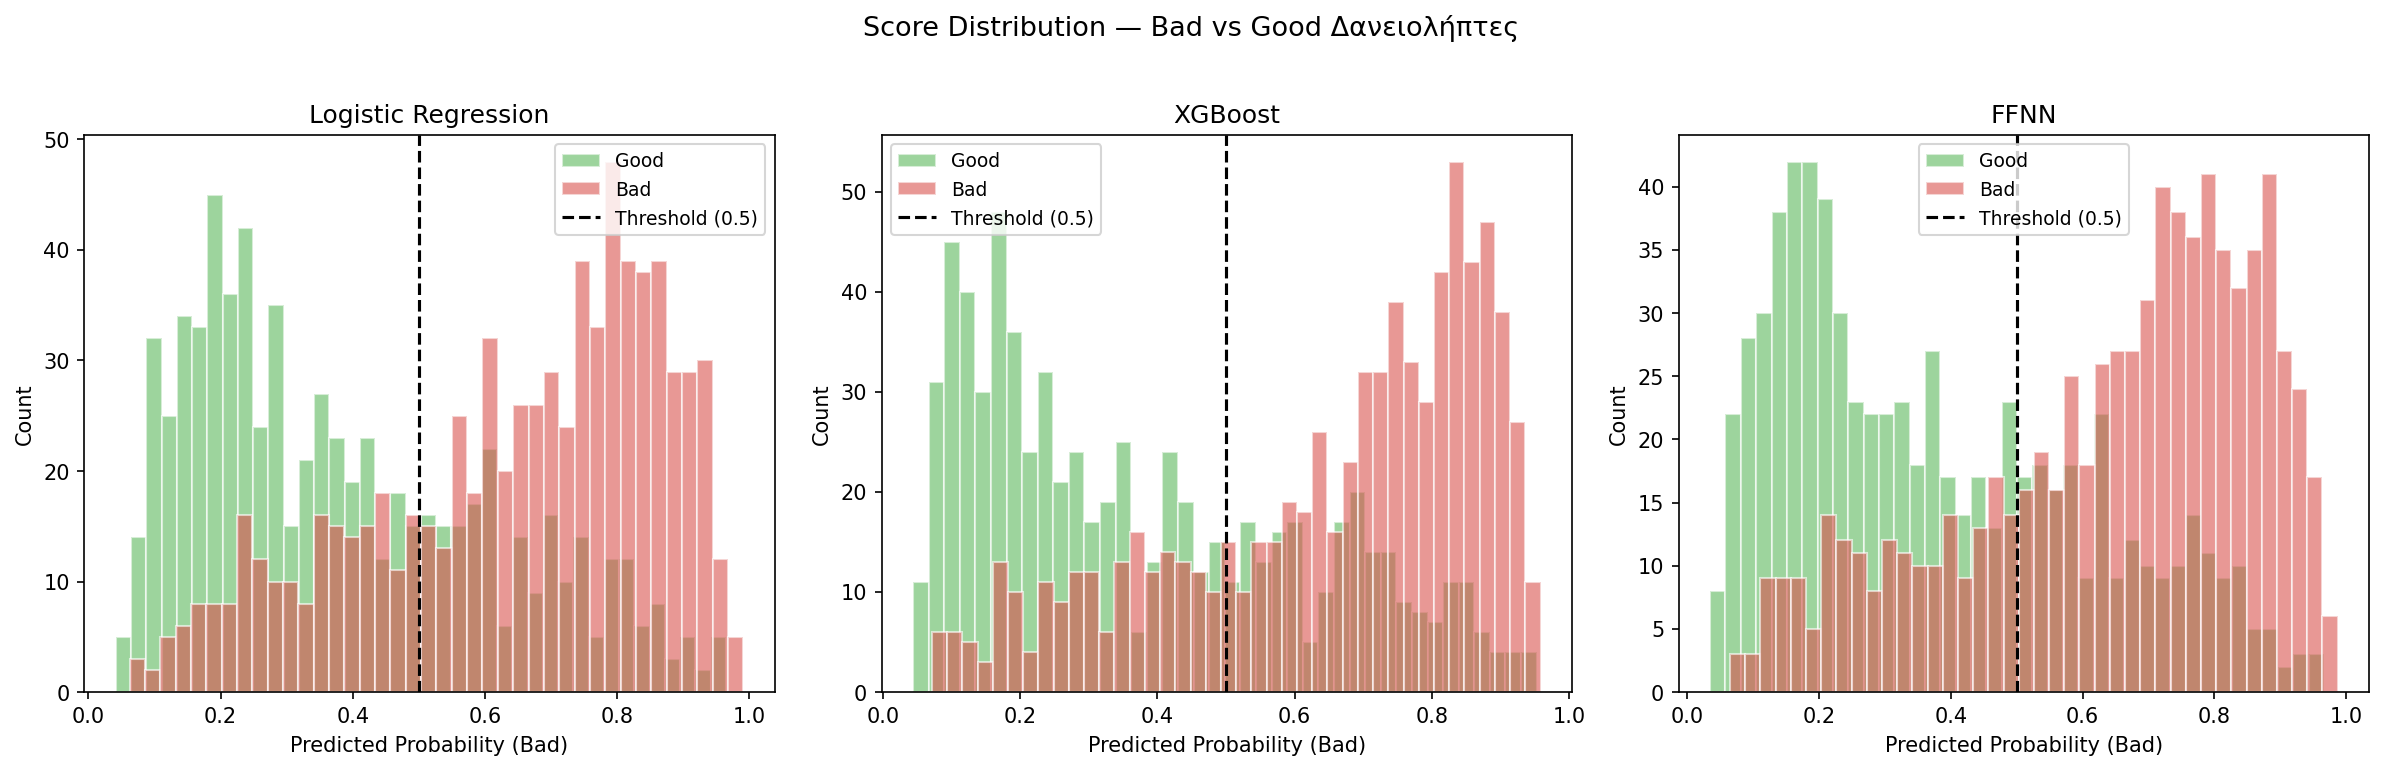
\includegraphics[width=\textwidth]{16_score_distribution}
    \caption[Κατανομή προβλεπόμενων πιθανοτήτων ανά μοντέλο]{Κατανομή προβλεπόμενων πιθανοτήτων για Bad
    (κόκκινο) και Good (πράσινο) δανειολήπτες για τα τρία
    μοντέλα. Η επικάλυψη των δύο κατανομών αντικατοπτρίζει
    την αβεβαιότητα ταξινόμησης και είναι συνεπής με τις
    οριακές διαφορές AUC των μοντέλων.}
    \label{fig:score_distribution}
\end{figure}


%--------------------------------------------------------------
\subsection{Έλεγχος Υπερπροσαρμογής}
\label{subsec:overfitting}

Ο Πίνακας~\ref{tab:overfitting} περιέχει την απόδοση των
μοντέλων στο training set, στο validation set αλλά και το
ποσοστό της σχετικής του πτώσης.
Το ποσοστό αυτό αποτελεί βασικό εργαλείο για τον έλεγχο
υπερπροσαρμογής (overfitting), ενώ το όριο που
χρησιμοποιείται στην παρούσα εργασία είναι το 5\%.
Η βιβλιογραφία δεν ορίζει αυστηρό κατώφλι· τιμές μεταξύ 5\%--10\% θεωρούνται 
συνήθως πρακτικά αποδεκτές για μοντέλα με ικανότητα γενίκευσης 
\citep{cawley2010over}.
Το XGBoost είναι το μόνο μοντέλο που ξεπερνά ελαφρώς
το όριο.
Το αποτέλεσμα αυτό είναι αναμενόμενο καθώς εμφανίζεται
σε μεγάλο ποσοστό στα μοντέλα δένδρων αποφάσεων \citep{chen2016xgboost, hastie2009}.
Οι τεχνικές αντιμετώπισης που εφαρμόστηκαν ---
Early stopping και stochastic regularization μέσω
δειγματοληψίας δεδομένων και χαρακτηριστικών ---
είναι αρκετές για την αντιμετώπισή του καθώς η απόλυτη
διαφορά στην απόδοση ανάμεσα στα δύο sets είναι
μικρή (0{,}806 vs 0{,}796).
Τα υπόλοιπα μοντέλα βρίσκονται αρκετά κάτω του ορίου
με σχετικές τιμές 1{,}3\% και 2{,}6\%.
Συμπερασματικά, τα μοντέλα έχουν την ικανότητα να
γενικοποιούν τις πληροφορίες του training set και να
τις εφαρμόζουν ικανοποιητικά σε διαφορετικά δεδομένα.

\begin{table}[htbp]
    \centering
    \caption[Έλεγχος υπερπροσαρμογής — Train/Val AUC]{Έλεγχος υπερπροσαρμογής --- σύγκριση Train/Val AUC
    και σχετική πτώση ανά μοντέλο.}
    \label{tab:overfitting}
    \begin{tabular}{lcccc}
        \toprule
        \textbf{Μοντέλο} & \textbf{Train AUC} & \textbf{Val AUC}
        & \textbf{Διαφορά} & \textbf{Σχετική Πτώση} \\
        \midrule
        Logistic Regression & 0{,}802 & 0{,}791 & 0{,}011 & 1{,}3\% \\
        XGBoost             & 0{,}859 & 0{,}806 & 0{,}053 & 6{,}2\% \\
        FFNN                & 0{,}819 & 0{,}798 & 0{,}021 & 2{,}6\% \\
        \bottomrule
    \end{tabular}
\end{table}

%--------------------------------------------------------------
\subsection{Πίνακες Σύγχυσης και Ανάλυση Ορίου}
\label{subsec:confusion_threshold}

% 15_confusion_matrices.png
Οι Πίνακες Σύγχυσης του Σχήματος~\ref{fig:confusion_matrices}
παρουσιάζουν τις κατηγοριοποιήσεις TP, TN, FP και FN που
περιεγράφηκαν στην ενότητα~\ref{subsec:metrics} για κάθε
μοντέλο για προεπιλεγμένο threshold $0{,}5$.
Στον πιστωτικό κίνδυνο υπάρχει ασυμμετρία κόστους ανάμεσα
στα λάθη FN και FP με τα πρώτα να κοστίζουν περισσότερο
στους δανειοδότες.
Στη συγκεκριμένη τιμή threshold το μοντέλο Logistic Regression
έχει τη χειρότερη απόδοση στην κατηγορία FN ενώ το XGBoost
την καλύτερη.
Το αποτέλεσμα αυτό δείχνει ελαφρώς καλύτερη απόδοση του
XGBoost αλλά δεν μπορεί να γενικοποιηθεί για όλες τις
τιμές threshold.

% -------------------------------------------------------------------
% Σχήμα 4.4 — Confusion Matrices τριών μοντέλων (NB02)
% Τοποθέτηση: αμέσως μετά το κείμενο ανάλυσης
% -------------------------------------------------------------------
\begin{figure}[htbp]
    \centering
    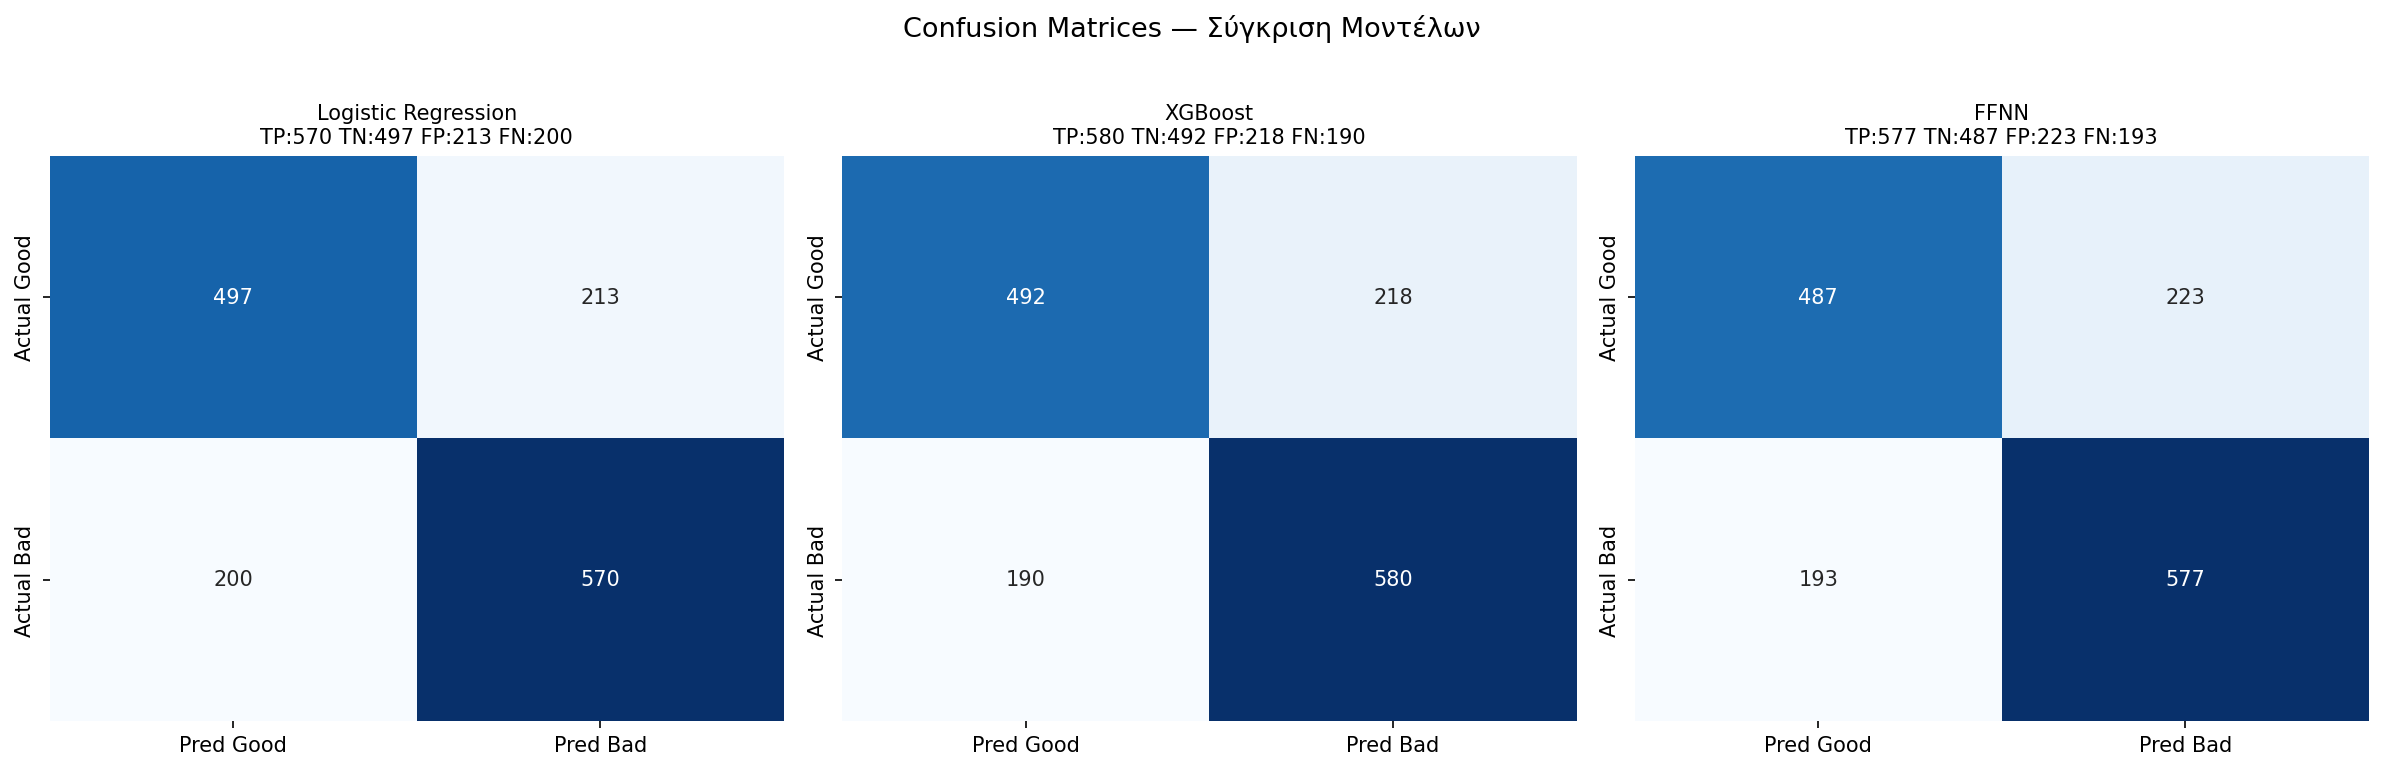
\includegraphics[width=\textwidth]{15_confusion_matrices}
    \caption[Πίνακες σύγχυσης τριών μοντέλων]{Πίνακες σύγχυσης για τα τρία μοντέλα στο test set
    με threshold $0{,}5$. Το XGBoost εμφανίζει τον μικρότερο
    αριθμό FN (190), γεγονός που αντιστοιχεί στο χαμηλότερο
    κόστος λάθους για τον δανειοδότη.}
    \label{fig:confusion_matrices}
\end{figure}

% 18_threshold_analysis.png
Η επιλογή του threshold αποτελεί επιχειρηματική απόφαση
καθώς πρέπει να είναι προσανατολισμένη με την πολιτική
της τράπεζας και το επιτρεπόμενο ρίσκο που διατίθεται
να αναλάβει.
Στο Σχήμα~\ref{fig:threshold_analysis} φαίνονται οι τιμές
Precision (ποσοστό σωστά ταξινομημένων Bad από τους
προβλεπόμενους Bad) και Recall (ποσοστό Bad που εντοπίστηκαν
από το σύνολο των πραγματικών Bad) για όλες τις πιθανές
τιμές του threshold και για τα τρία μοντέλα.
Η μετρική F1 --- ο αρμονικός μέσος των Precision και
Recall --- δείχνει το βέλτιστο σημείο ισορροπίας.
Η διαφορά είναι αρκετή για να δώσει μια μικρή υπεροχή
στο μοντέλο XGBoost αλλά όχι να το καταστήσει σαφώς
ανώτερο.
Η ασυμμετρία κόστους πιθανώς να οδηγούσε μια τράπεζα
να διαλέξει μια τιμή κάτω του $0{,}5$ για μεγιστοποίηση
του Recall εις βάρος της Precision.

% -------------------------------------------------------------------
% Σχήμα 4.5 — Threshold Analysis τριών μοντέλων (NB02)
% Τοποθέτηση: αμέσως μετά το κείμενο ανάλυσης
% -------------------------------------------------------------------
\begin{figure}[htbp]
    \centering
    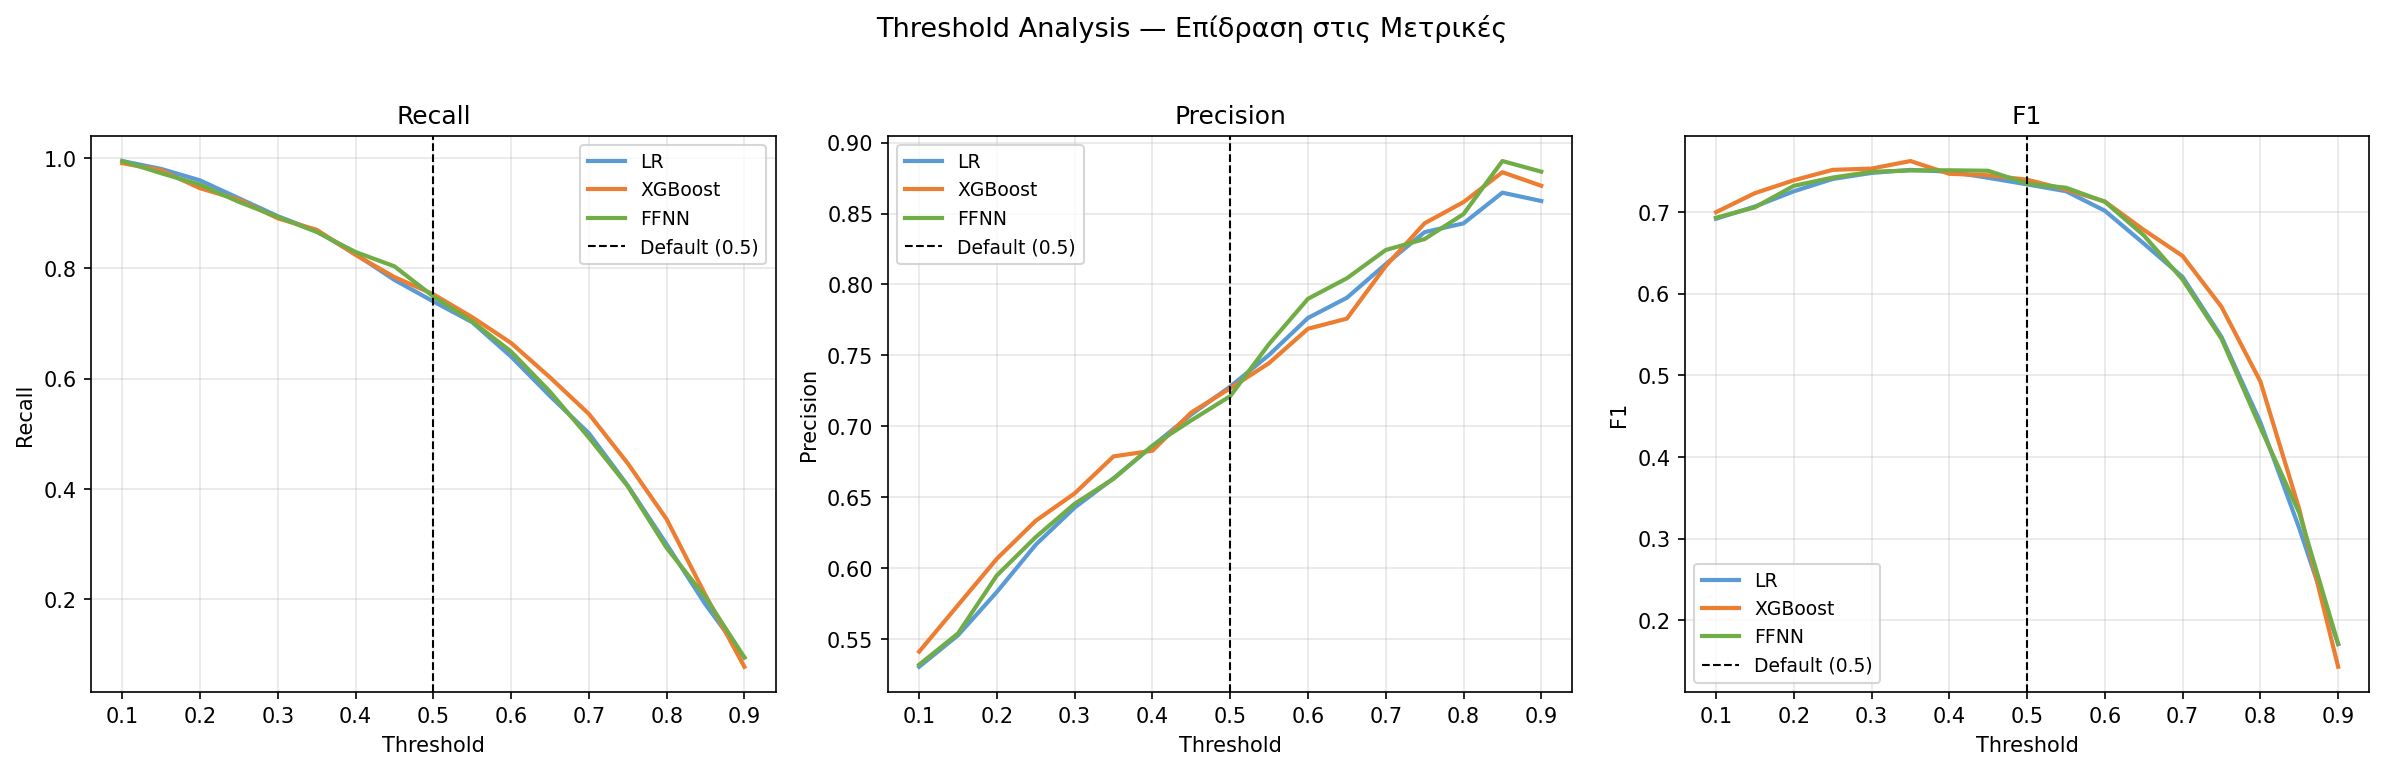
\includegraphics[width=\textwidth]{18_threshold_analysis}
    \caption[Threshold analysis τριών μοντέλων]{Επίδραση του threshold στις μετρικές Recall,
    Precision και F1 για τα τρία μοντέλα. Η κατακόρυφη
    διακεκομμένη γραμμή δείχνει το default threshold $0{,}5$.}
    \label{fig:threshold_analysis}
\end{figure}


%--------------------------------------------------------------
\subsection{Ανάλυση Κατά Δεκατημόρια}
\label{subsec:decile}

% 19_decile_analysis.png
Το Σχήμα~\ref{fig:decile_analysis} παρουσιάζει την ανάλυση
κατά δεκατημόρια για τα τρία μοντέλα.
Στο αριστερό μέρος του οπτικοποιείται το Bad Rate ανά
δεκατημόριο ενώ στο δεξί το αθροιστικό ποσοστό Bad
(Cumulative Bad Rate) σε σύγκριση με την τυχαία βασική
γραμμή, από την οποία τα μοντέλα σαφώς αποκλίνουν.
Οι τράπεζες απαιτούν στην decile analysis των αλγορίθμων
τα χειρότερα deciles να συγκεντρώνουν τον υψηλότερο κίνδυνο.
Η κατάταξη είναι ικανοποιητική με μη σημαντικές αριθμητικές διαφορές μεταξύ των αλγορίθμων.
Το εύρημα αυτό επιβεβαιώνει την προβλεπτική ικανότητα
των μοντέλων στον πιστωτικό κίνδυνο.

% -------------------------------------------------------------------
% Σχήμα 4.6 — Decile Analysis τριών μοντέλων (NB02)
% Τοποθέτηση: αμέσως μετά το κείμενο ανάλυσης
% -------------------------------------------------------------------
\begin{figure}[htbp]
    \centering
    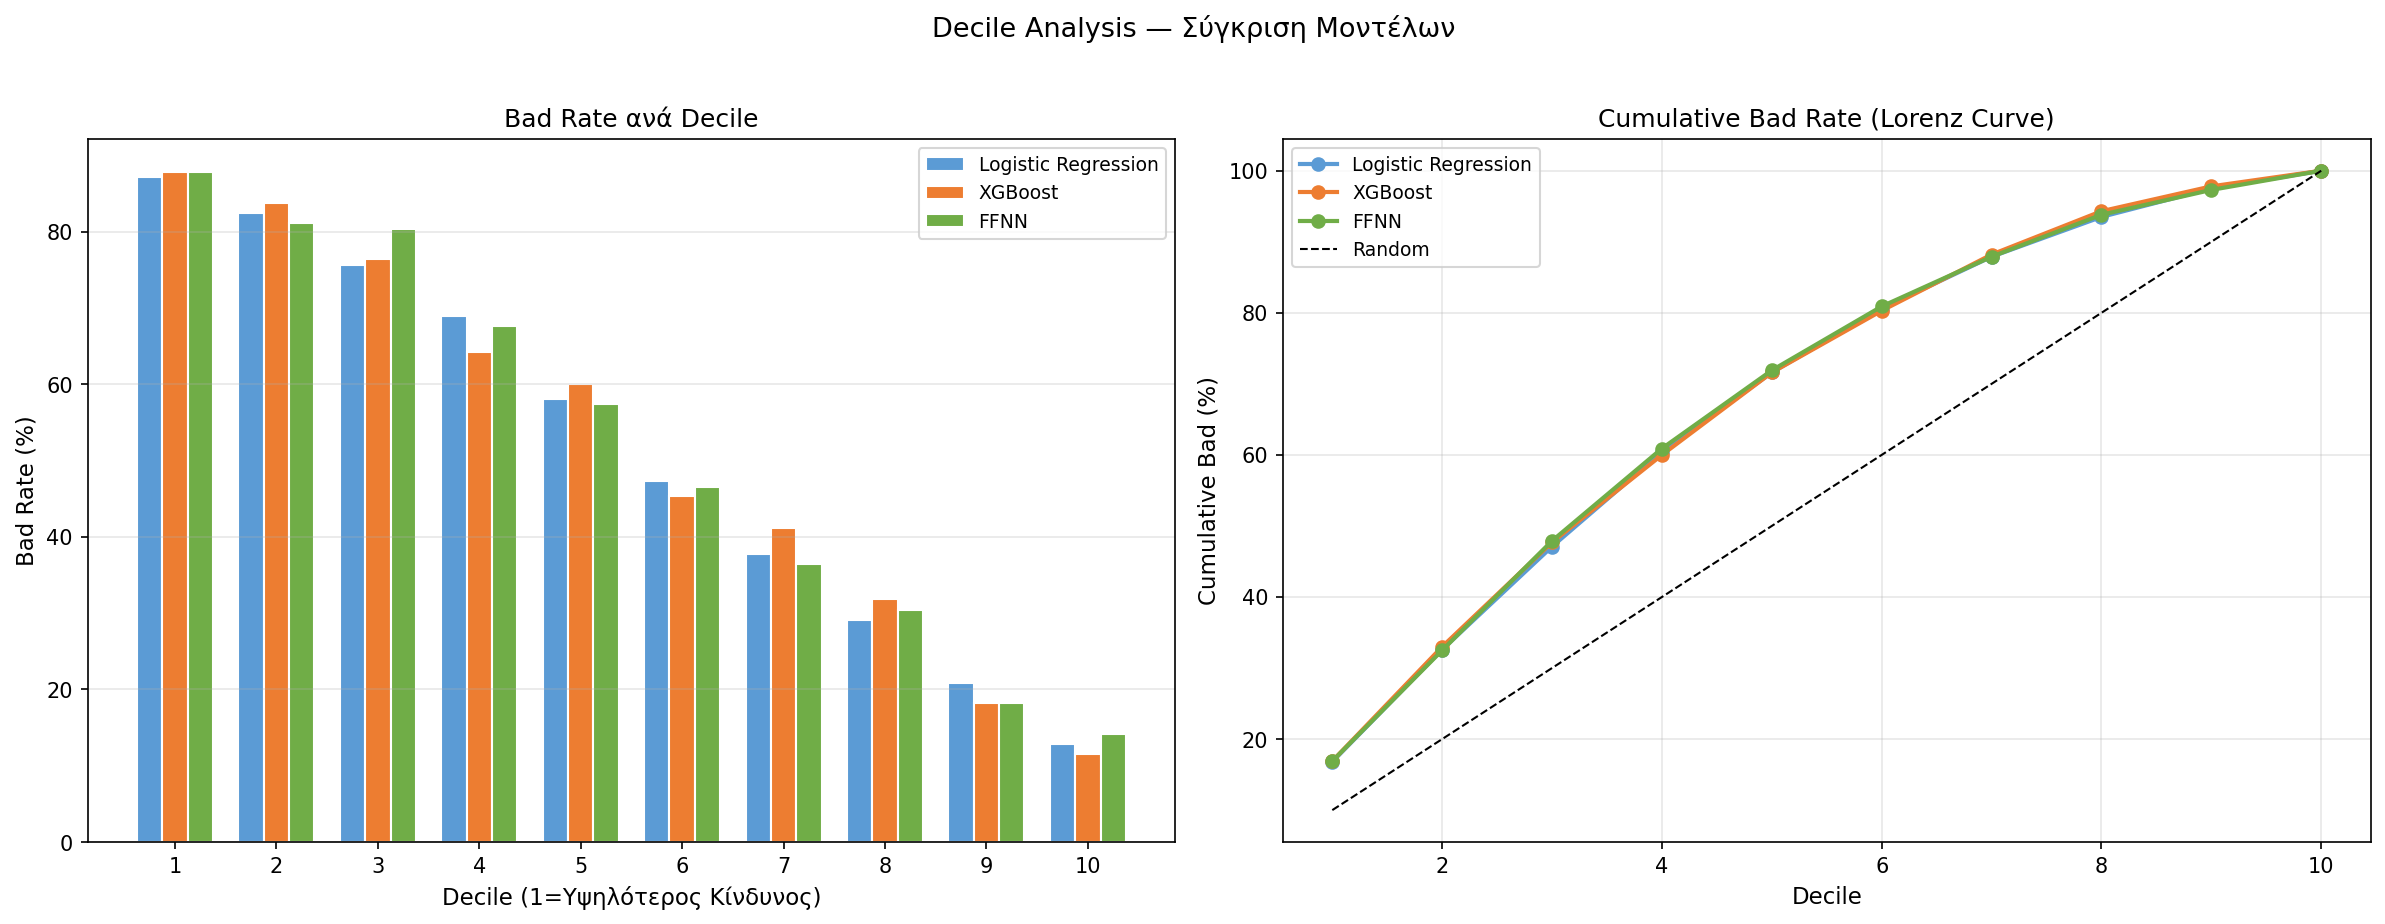
\includegraphics[width=\textwidth]{19_decile_analysis}
    \caption[Decile analysis τριών μοντέλων]{Ανάλυση κατά δεκατημόρια για τα τρία μοντέλα.
    Αριστερά: Bad Rate ανά decile — τα πρώτα deciles
    συγκεντρώνουν τον υψηλότερο κίνδυνο.
    Δεξιά: Cumulative Bad Rate σε σύγκριση με τη διαγώνιο
    τυχαίας πρόβλεψης.}
    \label{fig:decile_analysis}
\end{figure}



\subsection{Βαθμονόμηση Μοντέλων}
\label{subsec:calibration}

% 22_calibration.png
Το Σχήμα~\ref{fig:calibration} παρουσιάζει τα διαγράμματα βαθμονόμησης
και των τριών μοντέλων.
Τα αποτελέσματα διαφέρουν από αυτά της μετρικής AUC καθώς εξετάζεται
κάθε αλγόριθμος μεμονωμένα σε κάθε διάστημα πιθανοτήτων.
Η διαγώνια διακεκομμένη γραμμή συμβολίζει την τέλεια βαθμονόμηση.
Όταν η απόδοση ενός μοντέλου την ξεπερνά αυτό μεταφράζεται σε
υπερεκτίμηση κινδύνου ενώ το αντίθετο σε υποεκτίμηση.
Συγκεκριμένα, η Logistic Regression ακολουθεί πιστά την διαγώνιο
σε όλο το εύρος τιμών με μια μικρή υπερεκτίμηση στα υψηλά επίπεδα
($>0{,}8$) η οποία είναι όμως αμελητέα.
XGBoost παρουσιάζει μια ζώνη υπερεκτίμησης κινδύνου στο διάστημα
$(0\text{--}0{,}4)$ και ένα διάστημα ηπιότερης υποεκτίμησης στο
διάστημα $(0{,}6\text{--}1)$.
Το διάγραμμα του FFNN εμφανίζει την πιο ακανόνιστη συμπεριφορά
από τα τρία με αιχμές, ενώ η εγκυρότητά του φαίνεται να είναι
καλύτερη στις ακραίες τιμές του συνόλου.
Τα αποτελέσματα συμφωνούν σε μεγάλο βαθμό με την βιβλιογραφία
στην οποία παρατηρείται τάση συμπίεσης πιθανοτήτων προς το κέντρο
για τα μοντέλα δένδρων~\citep{niculescu2005predicting}.
XGBoost εμφανίζει τάση υπερεκτίμησης κυρίως στα χαμηλά και
μεσαία επίπεδα.
Τέλος, η Logistic Regression είναι η πιο αξιόπιστα βαθμονομημένη,
γεγονός που εξηγείται από την εκπαίδευσή της με log-loss
(cross-entropy) που τιμωρεί τις αποκλίσεις πιθανότητας.
Έτσι καθίσταται καταλληλότερη για υπολογισμό PD στο πλαίσιο
Basel~\citep{basel2017}.

% -------------------------------------------------------------------
% Σχήμα 4.6 — Calibration Plots (NB02)
% Τοποθέτηση: αμέσως μετά την αναφορά στη βαθμονόμηση
% -------------------------------------------------------------------
\begin{figure}[htbp]
    \centering
    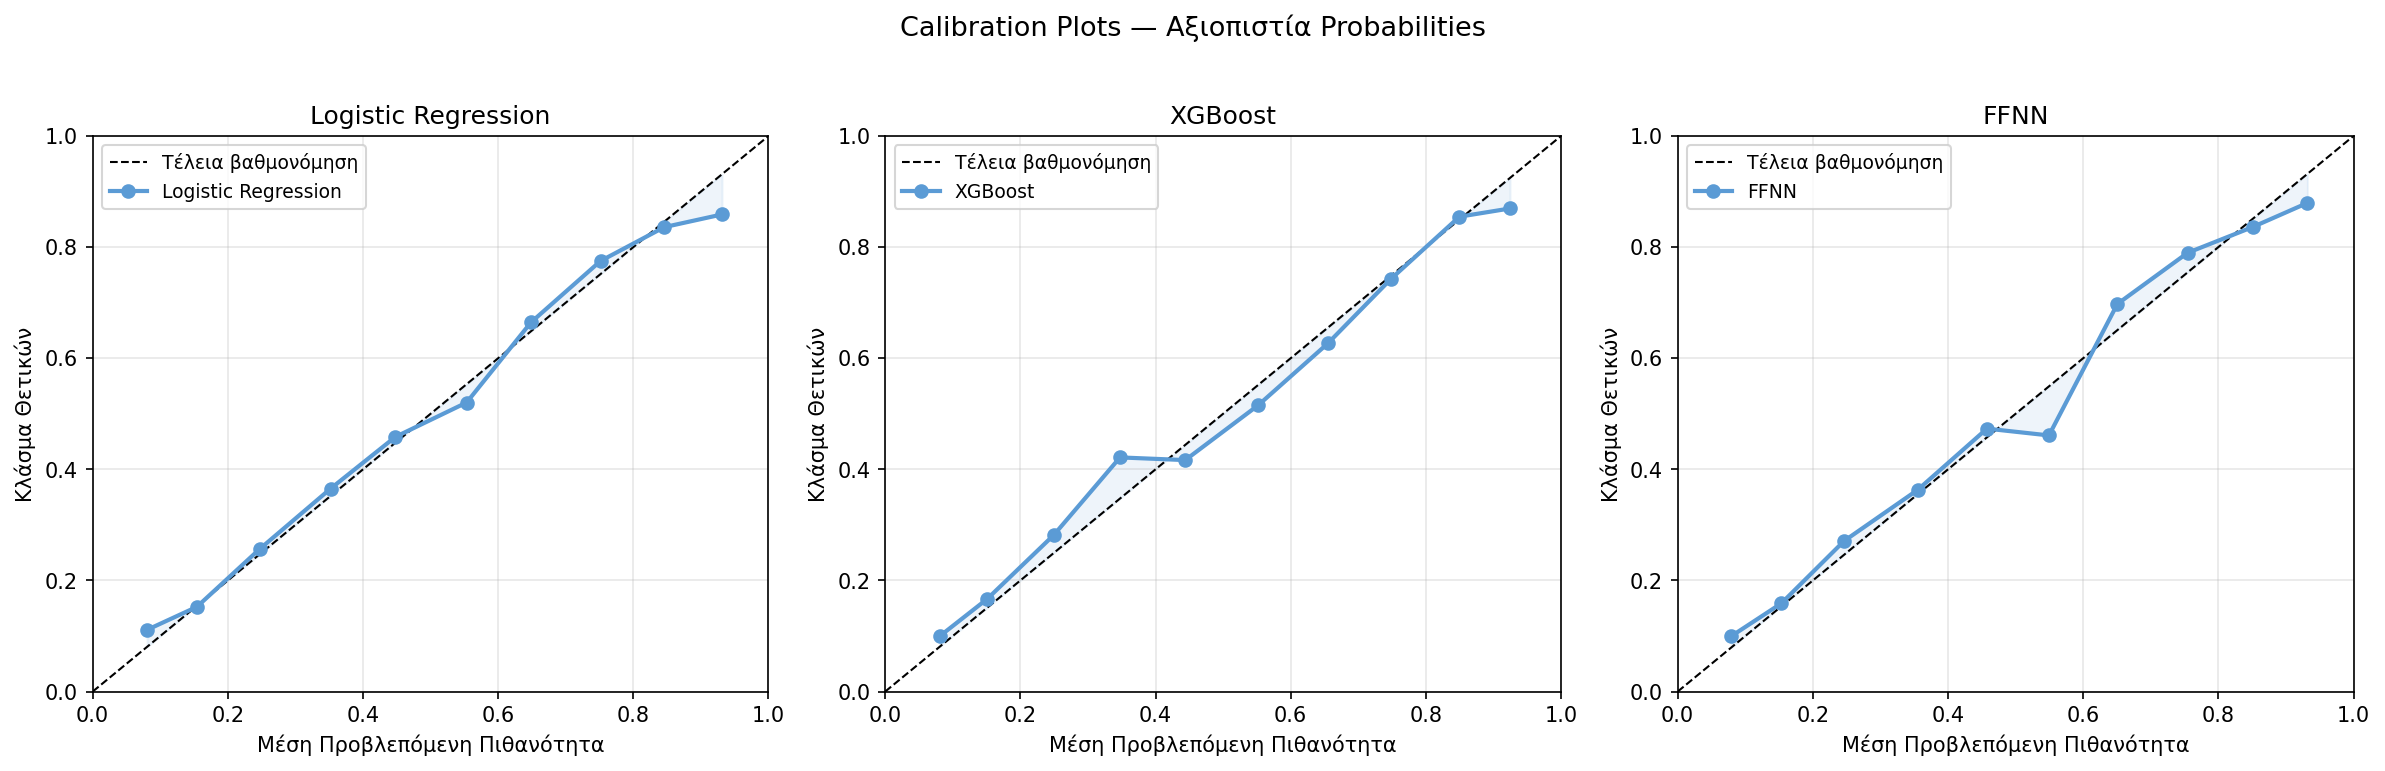
\includegraphics[width=\textwidth]{22_calibration}
    \caption[Διαγράμματα βαθμονόμησης τριών μοντέλων]{Διαγράμματα βαθμονόμησης των τριών μοντέλων. Η διαγώνιος
             αντιστοιχεί στην τέλεια αντιστοίχηση προβλεπόμενης πιθανότητας
             και παρατηρούμενου Bad Rate. Η βαθμονόμηση είναι απαραίτητη για
             την αξιόπιστη τιμολόγηση επιτοκίων και τον υπολογισμό εποπτικών
             κεφαλαίων (Basel III).}
    \label{fig:calibration}
\end{figure}



\section{Εξειδικευμένη Ανάλυση XGBoost}
\label{sec:results_xgboost}

\subsection{Ερμηνευσιμότητα SHAP --- Καθολικό Επίπεδο}
\label{sec:results_shap_global}

% 05_shap_feature_importance.png
Το Σχήμα~\ref{fig:shap_importance} παρουσιάζει το Global SHAP Feature Importance
για το XGBoost.
Όπως αναφέρθηκε στην ενότητα~\ref{sec:shap}, η Global SHAP ορίζεται ως η μέση
απόλυτη τιμή SHAP για κάθε χαρακτηριστικό σε ολόκληρο το test set.
Οι μεταβλητές με την μεγαλύτερη τιμή είναι αυτές που επηρεάζουν περισσότερο
τις προβλέψεις του μοντέλου συνολικά.
Συγκεκριμένα, κορυφαίο χαρακτηριστικό αναδεικνύεται το
\texttt{ExternalRiskEstimate} --- συνθετικό χαρακτηριστικό της FICO ---
το οποίο προκύπτει από την σύνθεση πολλαπλών πληροφοριών πιστωτικής
συμπεριφοράς σε έναν αριθμό.
Ακολουθεί το \texttt{MSinceMostRecentInqexcl7days} --- δείκτης πρόσφατων
πιστωτικών ερευνών --- το ποσοστό χρήσης ανακυκλούμενης πίστωσης
\texttt{NetFractionRevolvingBurden}, ο δείκτης ηλικίας πιστωτικού
ιστορικού \texttt{AverageMInFile} και το ποσοστό πιστωτικών λογαριασμών
χωρίς καμία καθυστέρηση πληρωμής \texttt{PercentTradesNeverDelinq}.
Τα αποτελέσματα αυτά αποκαλύπτουν ότι το μοντέλο θεωρεί πιο έμπιστους
τους δανειολήπτες που κυρίως δεν ψάχνουν για μεγάλο χρονικό διάστημα
ενεργά για δάνειο, δεν προσεγγίζουν το όριο της πιστωτικής τους κάρτας,
έχουν παλαιό πιστωτικό ιστορικό και χωρίς καθυστέρηση στις πληρωμές τους.
Λιγότερη βαρύτητα έχουν οι μεταβλητές \texttt{MSinceMostRecentTradeOpen}
και \texttt{NumTotalTrades}, διότι χαρακτηριστικά όπως οι μήνες από το
άνοιγμα του πιο πρόσφατου πιστωτικού λογαριασμού και ο συνολικός αριθμός
πιστωτικών λογαριασμών του δανειολήπτη έχουν περιορισμένη αυτόνομη
προβλεπτική ισχύ.
Η μειωμένη σημαντικότητά τους μπορεί εν μέρει να εξηγηθεί και από
επικάλυψη πληροφορίας με σημαντικότερα features.

% -------------------------------------------------------------------
% Σχήμα 4.7 — SHAP Feature Importance (NB03)
% Τοποθέτηση: αμέσως μετά τα αποτελέσματα Global SHAP
% -------------------------------------------------------------------
\begin{figure}[htbp]
    \centering
    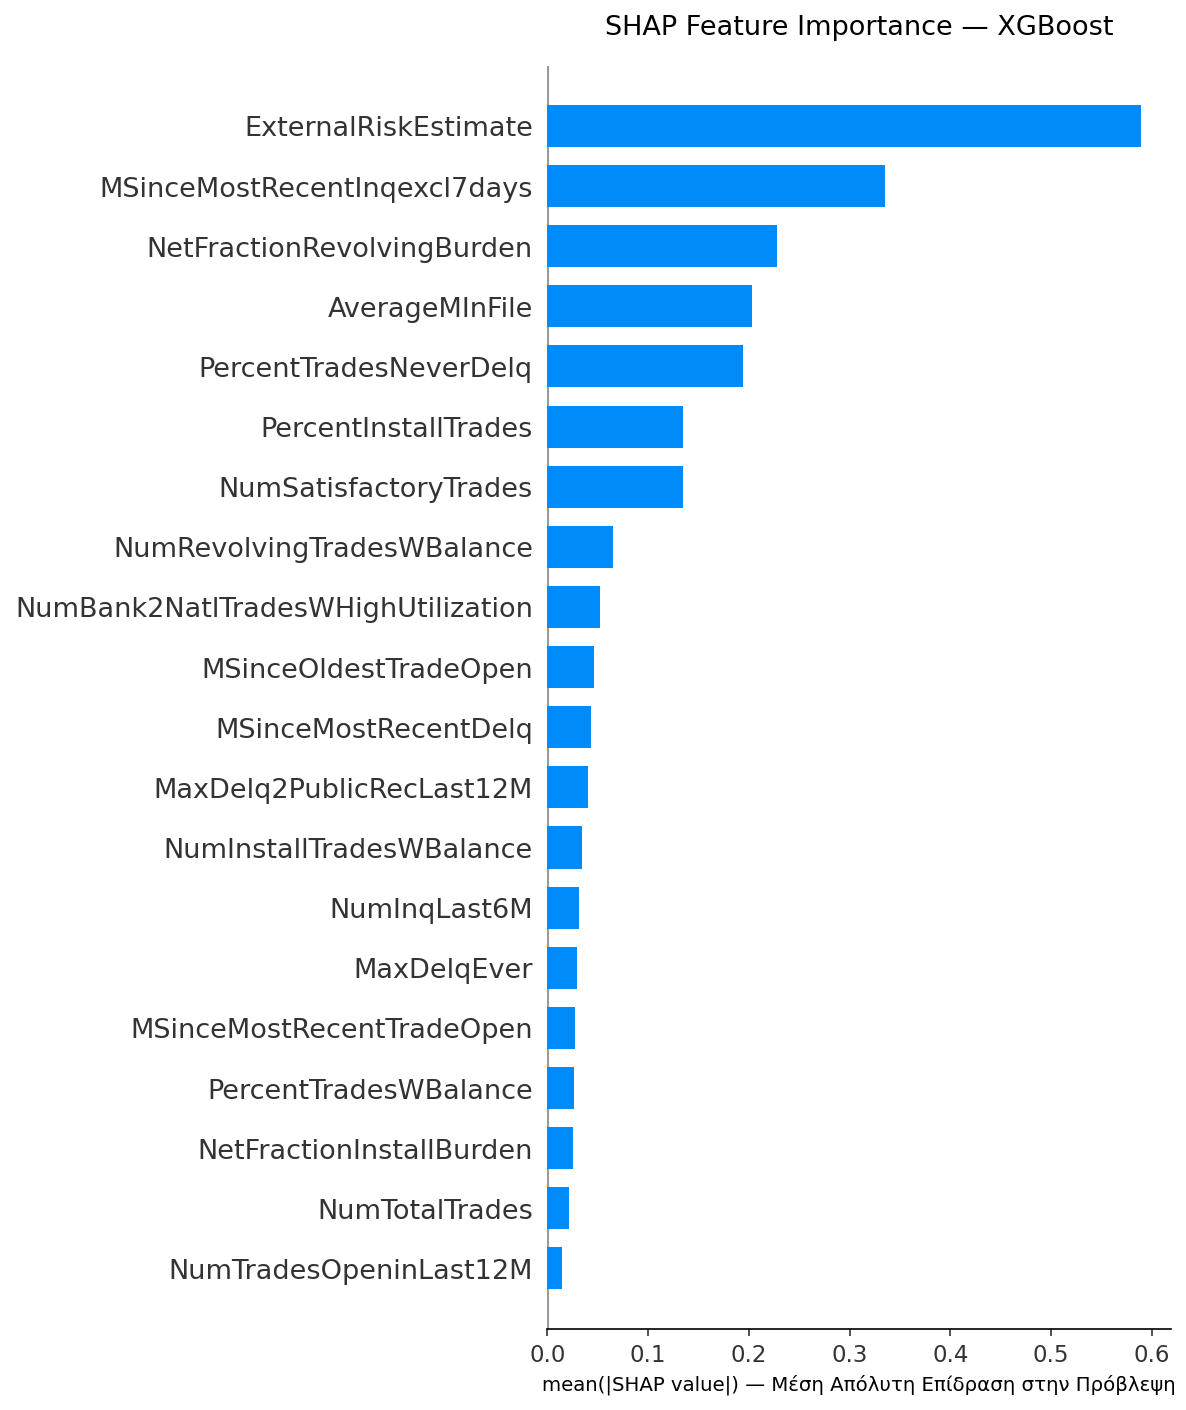
\includegraphics[width=0.80\textwidth]{05_shap_feature_importance}
    \caption[SHAP Global Feature Importance — XGBoost]{SHAP Global Feature Importance για το XGBoost. Το mean(|SHAP value|)
             κάθε χαρακτηριστικού εκφράζει τη μέση συνεισφορά του στις
             προβλέψεις. Κορυφαίο χαρακτηριστικό το \texttt{ExternalRiskEstimate},
             ακολουθούμενο από δείκτες πρόσφατης πιστωτικής δραστηριότητας
             και χρέους.}
    \label{fig:shap_importance}
\end{figure}

% 06_shap_summary.png
Το Σχήμα~\ref{fig:shap_summary} παρουσιάζει το Beeswarm διάγραμμα
για το μοντέλο XGBoost.
Το παρόν διάγραμμα προσθέτει κατεύθυνση και κατανομή στο μονοδιάστατο
bar chart του Σχήματος~\ref{fig:shap_importance}.
Κάθε τελεία αντιστοιχεί σε μια εγγραφή του test set και το χρώμα της
δείχνει αν η τιμή του χαρακτηριστικού είναι υψηλή (κόκκινο) ή χαμηλή (μπλε).
Η σειρά των μεταβλητών είναι με βάση τη σημαντικότητά τους ενώ η
συντεταγμένη κάθε τελείας στον άξονα x δείχνει την SHAP τιμή της,
δηλαδή το πόσο και κατά ποιον τρόπο επηρεάζει την τελική πρόβλεψη.
Για το \texttt{ExternalRiskEstimate} παρατηρείται σαφής διαχωρισμός
χρωμάτων στον άξονα x, όπως και για τα \texttt{NetFractionRevolvingBurden},
\texttt{AverageMInFile}, \texttt{PercentTradesNeverDelinq} και
\texttt{NumSatisfactoryTrades}.
Το γεγονός αυτό αποκαλύπτει ότι οι τιμές των αναφερθέντων μεταβλητών
αποτελούν ισχυρό κριτήριο για την τελική συνεισφορά τους στο ποσοστό επικινδυνότητας.
Αντίθετα, για τις μεταβλητές \texttt{MSinceMostRecentInqexcl7days},
\texttt{PercentInstallTrades}, \texttt{NumRevolvingTradesWBalance},
\texttt{MSinceMostRecentDelq} και \texttt{NumTradesOpenInLast12M}
παρατηρείται έντονη ανάμειξη χρωμάτων.
Η τιμή των μεταβλητών δεν καθορίζει την SHAP τιμή τους με αποτέλεσμα
δανειολήπτες με ίδια τιμή στις μεταβλητές να επηρεάζονται διαφορετικά.
Το φαινόμενο έχει τρεις πιθανές εξηγήσεις που για κάθε μεταβλητή
μπορεί να διαφέρει: η αλληλεπίδραση με άλλα χαρακτηριστικά του
δανειολήπτη, η χαμηλή προβλεπτική ισχύς του χαρακτηριστικού που
δεν επιτρέπει την ξεκάθαρη συσχέτισή του με τον κίνδυνο, ή η μη
μονότονη σχέση του με αυτόν.
Τα συμπεράσματα από το διάγραμμα είναι σημαντικά για την
ερμηνευσιμότητα του μοντέλου, καθώς οπτικοποιείται η κατεύθυνση
και η ένταση επίδρασης κάθε χαρακτηριστικού και συμβάλλει στη
διαδικασία επεξηγηματικότητας προς τη συμμόρφωση με το κανονιστικό
πλαίσιο~\citep{eba2023}.

% -------------------------------------------------------------------
% Σχήμα 4.8 — SHAP Beeswarm Plot XGBoost (NB03)
% Τοποθέτηση: αμέσως μετά το κείμενο ανάλυσης
% -------------------------------------------------------------------
\begin{figure}[htbp]
    \centering
    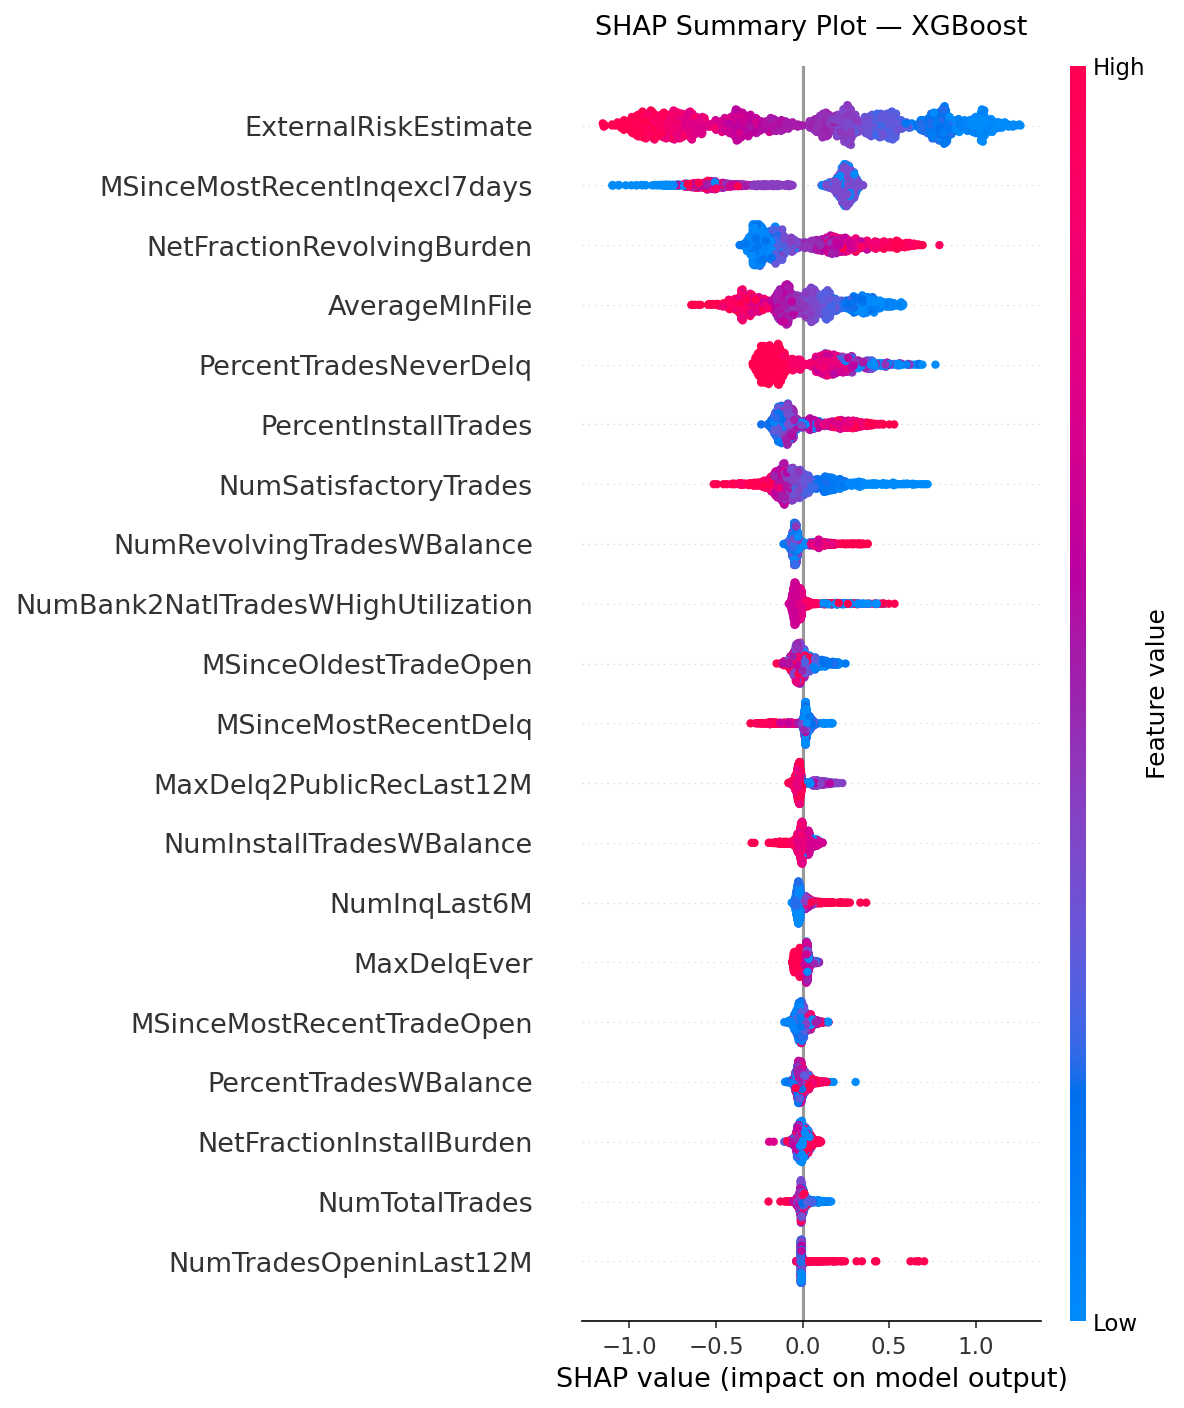
\includegraphics[width=\textwidth]{06_shap_summary}
    \caption[SHAP Beeswarm Plot — XGBoost]{SHAP Beeswarm Plot για το XGBoost. Κάθε τελεία αντιστοιχεί
             σε έναν δανειολήπτη του test set. Το χρώμα δείχνει την τιμή
             του χαρακτηριστικού (κόκκινο = υψηλή, μπλε = χαμηλή) και η
             θέση στον άξονα x την κατεύθυνση και ένταση επίδρασής του
             στην πρόβλεψη.}
    \label{fig:shap_summary}
\end{figure}

\subsection{Ερμηνευσιμότητα SHAP --- Τοπικό Επίπεδο}
\label{sec:results_shap_local}

% 07_shap_local_bad.png, 08_shap_local_good.png
Όπως αναφέρθηκε και σε προηγούμενες παραγράφους ο κανονισμός GDPR \citep{goodman2017european} και οι
κατευθύνσεις της EBA \citep{eba2023} προστατεύουν το «δικαίωμα εξήγησης» των υποψηφίων
δανειοληπτών.
Τα Σχήματα~\ref{fig:shap_local_bad} και~\ref{fig:shap_local_good} ικανοποιούν
συγκεκριμένα αυτό το δικαίωμα.
Παρουσιάζονται δύο SHAP Waterfall plots, ένα για Bad και ένα για Good δανειολήπτη.
Για κάθε δανειολήπτη το διάγραμμα ξεκινά από την τιμή 0{,}0 του άξονα x
ο οποίος συμβολίζει το base value, δηλαδή τη μέση πρόβλεψη του μοντέλου.
Κάθε χαρακτηριστικό μετατοπίζει την πρόβλεψη προς τα δεξιά (αυξάνει τον
κίνδυνο) ή αριστερά (μειώνει τον κίνδυνο).
Η σύγκριση ανάμεσα στα δύο διαγράμματα αποκαλύπτει την συλλογιστική
πορεία του μοντέλου.

Για τον Bad δανειολήπτη φαίνεται ότι η μεταβλητή
\texttt{ExternalRiskEstimate}=58 κυριαρχεί στο αποτέλεσμα μετατοπίζοντας
το αποτέλεσμα κατά απόλυτη τιμή 3 φορές περισσότερο από την δεύτερη
μεγαλύτερη μετατόπιση.
Ενώ οι πέντε από τις εννέα πιο σημαντικές μεταβλητές αφαιρούν από το
σκορ επικινδυνότητας του, η τελική τιμή $f(x) = 1{,}059$ (log-odds)
αντιστοιχεί σε υψηλή πιθανότητα αθέτησης.
Για τον Good δανειολήπτη φαίνεται μια συμφωνία στις ισχυρότερες μεταβλητές
με εφτά από τις εννέα να μειώνουν την τελική τιμή $f(x)$ η οποία τελικά
είναι ίση με $-1{,}678$ (log-odds).
Από το διάγραμμα SHAP feature importance προέκυψε το συμπέρασμα ότι η
μεταβλητή \texttt{ExternalRiskEstimate} έχει την μεγαλύτερη σημαντικότητα
για το μοντέλο αλλά για τον συγκεκριμένο δανειολήπτη φαίνεται να μην
επηρεάζει τόσο το τελικό αποτέλεσμα αλλά ούτε να συμφωνεί κατά πρόσημο
με αυτό.
Το \texttt{ExternalRiskEstimate} για τον Good δανειολήπτη έχει θετική SHAP
τιμή (σπρώχνει προς Bad) παρότι ο δανειολήπτης είναι Good --- αυτό δείχνει
ότι άλλα features αντισταθμίζουν την επίδρασή του.
Επιπλέον, η απόλυτη μετατόπιση που προκαλεί στην $f(x)$ είναι όγδοη κατά
φθίνουσα σειρά ίση με $0{,}11$ σε σύγκριση με το $+1$ για τον Bad.

% -------------------------------------------------------------------
% Σχήμα 4.9 — SHAP Waterfall Bad δανειολήπτης (NB03)
% Τοποθέτηση: αμέσως μετά το κείμενο ανάλυσης
% -------------------------------------------------------------------
\begin{figure}[htbp]
    \centering
    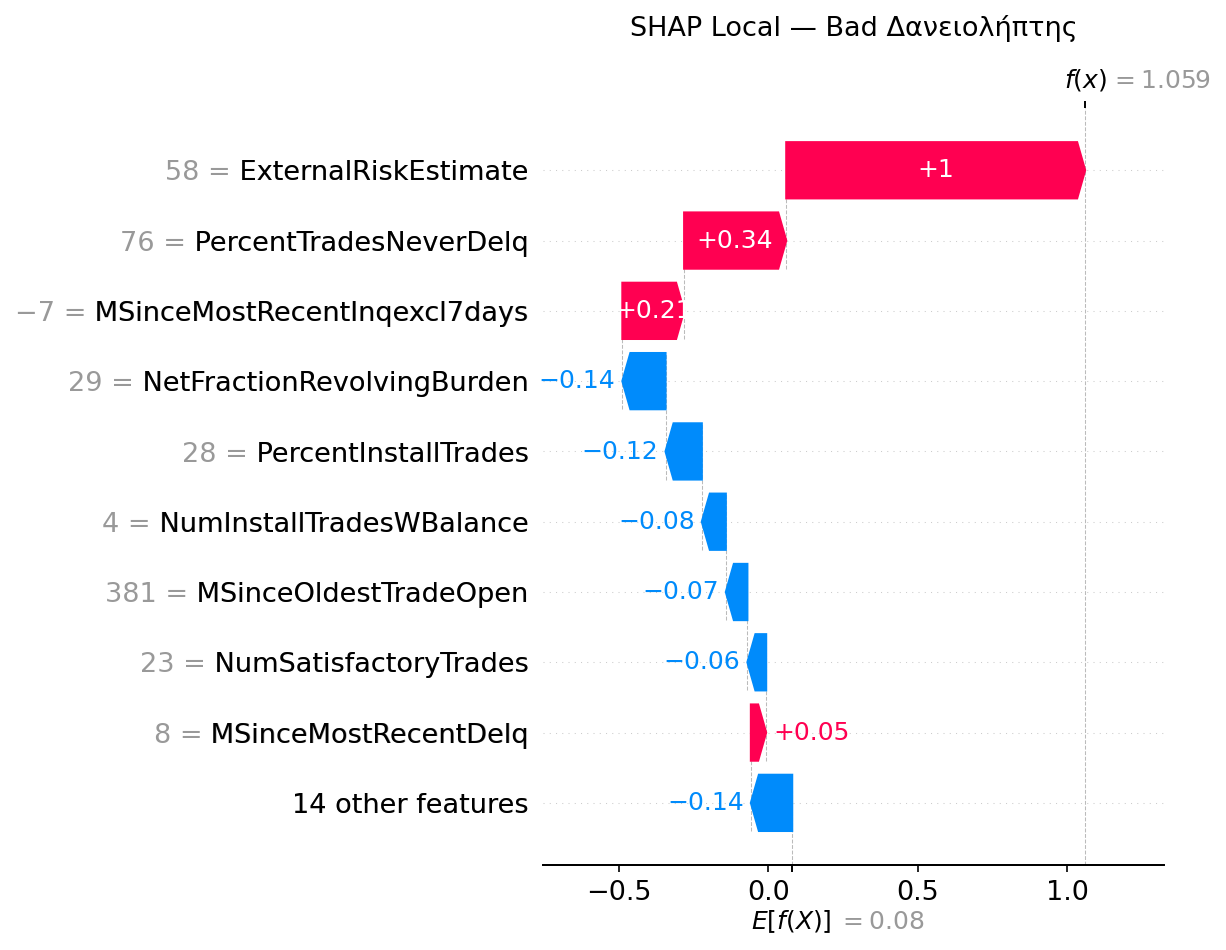
\includegraphics[width=\textwidth]{07_shap_local_bad}
    \caption[SHAP Waterfall — Bad δανειολήπτης]{SHAP Waterfall plot για Bad δανειολήπτη. Το
             \texttt{ExternalRiskEstimate}=58 κυριαρχεί στην πρόβλεψη
             με μετατόπιση τριπλάσια από το δεύτερο feature.
             Τελική πρόβλεψη $f(x)=1{,}059$ (log-odds).}
    \label{fig:shap_local_bad}
\end{figure}

% -------------------------------------------------------------------
% Σχήμα 4.10 — SHAP Waterfall Good δανειολήπτης (NB03)
% Τοποθέτηση: αμέσως μετά το Bad waterfall
% -------------------------------------------------------------------
\begin{figure}[htbp]
    \centering
    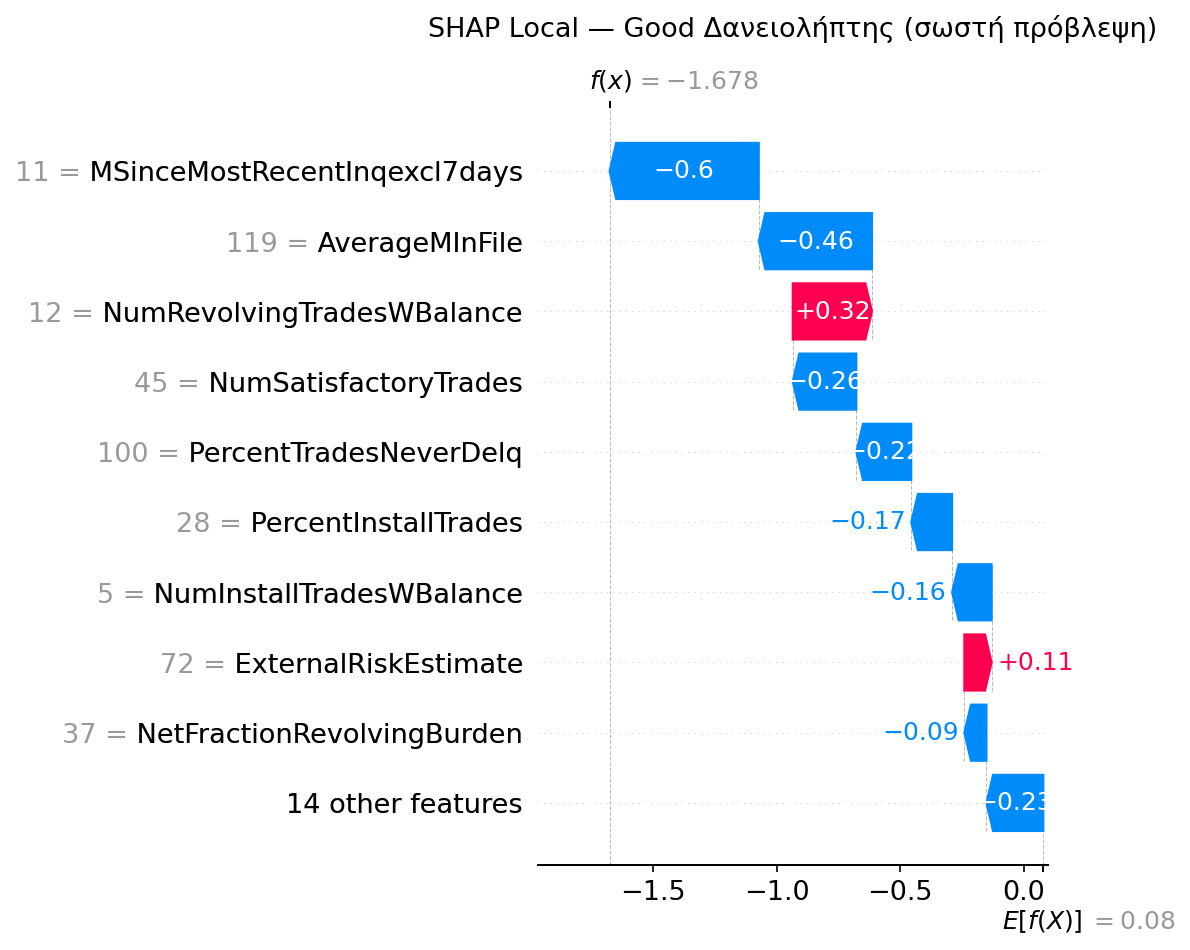
\includegraphics[width=\textwidth]{08_shap_local_good}
    \caption[SHAP Waterfall — Good δανειολήπτης]{SHAP Waterfall plot για Good δανειολήπτη. Εφτά από τις
             εννέα κορυφαίες μεταβλητές μειώνουν τον κίνδυνο.
             Τελική πρόβλεψη $f(x)=-1{,}678$ (log-odds).}
    \label{fig:shap_local_good}
\end{figure}


\subsection{Partial Dependence Plots}
\label{sec:results_pdp}

% 09_pdp.png
Το κανονιστικό πλαίσιο του τομέα διακρίνεται σε δύο επίπεδα.
Το πρώτο απαιτεί την απάντηση στο ερώτημα «γιατί έγινε η απόρριψη»
ενώ το δεύτερο στο ερώτημα «πως μπορεί να αλλάξει η απόφαση».
Τα Partial Dependence Plots του Σχήματος~\ref{fig:pdp} απαντούν
στο δεύτερο ερώτημα.
Τα PDP για τα τέσσερα κορυφαία χαρακτηριστικά αποκαλύπτουν πως
αυτά επηρεάζουν τη μέση πρόβλεψη, με τα υπόλοιπα χαρακτηριστικά
να παραμένουν σταθερά στη μέση τιμή τους.
Η παραδοχή αυτή για τα υπόλοιπα χαρακτηριστικά δεν μας παρέχει
την πλήρη εικόνα για την υποστήριξη actionable recourse καθώς
αγνοεί πιθανές αλληλεπιδράσεις ανάμεσα στα χαρακτηριστικά.
Αξίζει να σημειωθεί ότι η μεταβλητή
\texttt{MSinceMostRecentInqexcl7days} είναι η μόνη από τις 4 για
την οποία η τιμή της δεν αποτελεί ισχυρό κριτήριο για την τελική
συνεισφορά της στο ποσοστό επικινδυνότητας
(Σχήμα~\ref{fig:shap_summary}).
Έτσι η διατήρηση των υπόλοιπων μεταβλητών στην μέση τιμή τους
έχει μεγαλύτερη βαρύτητα στην ερμηνεία του διαγράμματος αυτής
της μεταβλητής καθώς όταν οι τιμές τους διαφοροποιηθούν είναι
πιθανόν να το επηρεάσουν.

Στα διαγράμματα βλέπουμε στον άξονα x τις τιμές της κάθε
μεταβλητής ενώ στον άξονα y την εξάρτηση της τελικής πρόβλεψης
από αυτά.
Στο διάγραμμα υπάρχει και rug plot με κατακόρυφα σημάδια στον
άξονα x να οπτικοποιούν την πυκνότητα των πραγματικών δειγμάτων.
Παρατηρείται ότι τα περισσότερα διαγράμματα δεν είναι αυστηρά
μονότονα ούτε γραμμικά αλλά οι πυκνότερες περιοχές αυτών θα
μπορούσαν να προσεγγιστούν με την χρήση γραμμικών, άρα και
αυστηρά μονότονων, συναρτήσεων.
Το γεγονός αυτό εξηγεί τα συγκρίσιμα αποτελέσματα στην απόδοση
της Logistic Regression με το XGBoost
(Πίνακας~\ref{tab:model_metrics}).
Στη διαδικασία προσέγγισης η μεταβλητή με την μεγαλύτερη απόκλιση
θα ήταν η \texttt{MSinceMostRecentInqexcl7days}, εύρημα που
ενισχύει τις υποθέσεις της προηγούμενης παραγράφου.
Συγκεκριμένα, το διάγραμμα της \texttt{ExternalRiskEstimate}
παρουσιάζει κορυφή ίση με $0{,}7$ στον άξονα y, είναι φθίνουσα
στο μεγαλύτερο διάστημά της με τις μικρότερες τιμές της να είναι
κοντά στο $0{,}35$.
Η \texttt{MSinceMostRecentInqexcl7days} ενώ αρχικά είναι αύξουσα,
στη συνέχεια παραμένει σταθερή για τιμές x από $-5$ μέχρι $1$
και έπειτα φθίνει.
Το πεδίο τιμών της είναι $(0{,}35\text{--}0{,}57)$.
Η \texttt{NetFractionRevolvingBurden} είναι κυρίως αύξουσα σε
όλο το πεδίο ορισμού της με ελάχιστη τιμή $0{,}47$ και μέγιστη
$0{,}63$.
Τέλος, η \texttt{AverageMInFile} παρουσιάζει φθίνουσα τάση και
παίρνει τιμές ανάμεσα στο $0{,}62$ και $0{,}46$.
Τα πεδία τιμών των μεταβλητών είναι παρόμοια, γεγονός που
επιβεβαιώνει τη συγκρίσιμη κατά απόλυτη τιμή επίδρασή τους
στην τελική πρόβλεψη.

% -------------------------------------------------------------------
% Σχήμα 4.11 — Partial Dependence Plots top-4 features XGBoost (NB03)
% Τοποθέτηση: αμέσως μετά το κείμενο ανάλυσης
% -------------------------------------------------------------------
\begin{figure}[htbp]
    \centering
    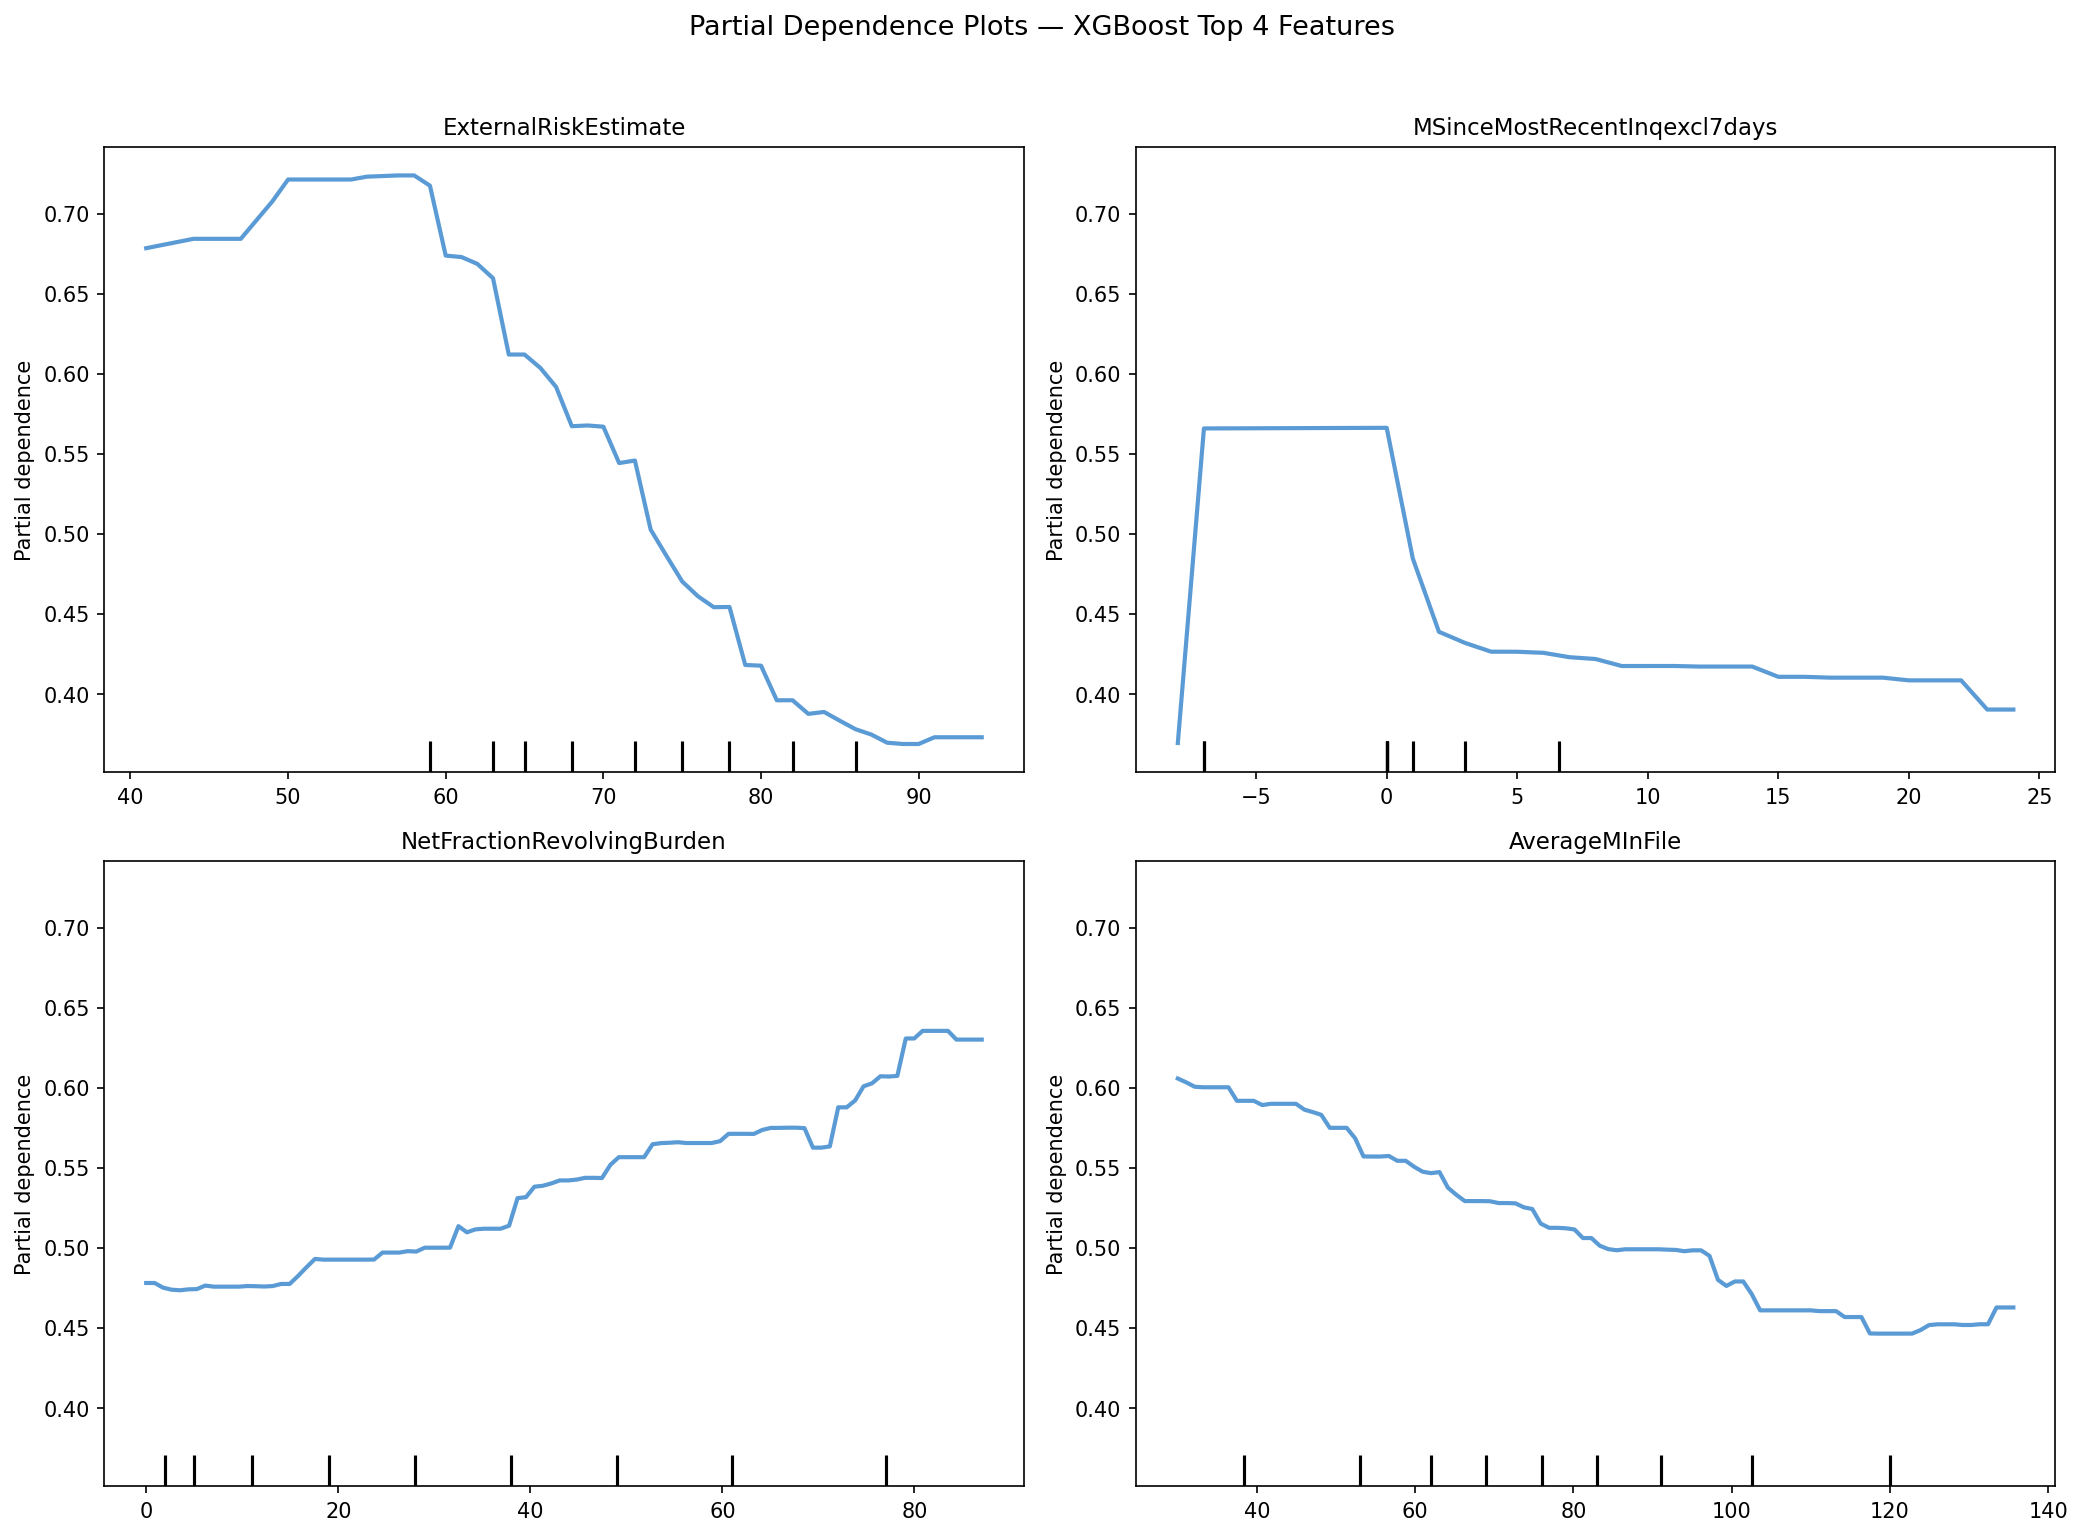
\includegraphics[width=\textwidth]{09_pdp}
    \caption[Partial Dependence Plots — top-4 χαρακτηριστικά]{Partial Dependence Plots για τα τέσσερα κορυφαία
             χαρακτηριστικά του XGBoost. Ο άξονας y δείχνει τη μέση
             προβλεπόμενη πιθανότητα Bad. Τα κατακόρυφα σημάδια στον
             άξονα x (rug plot) οπτικοποιούν την πυκνότητα των
             πραγματικών δειγμάτων.}
    \label{fig:pdp}
\end{figure}


\subsection{Ερμηνευσιμότητα SHAP για FFNN και Υπολογιστικό Κόστος}
\label{sec:results_ffnn_shap}

% 10_shap_ffnn_importance.png
Το Σχήμα~\ref{fig:shap_ffnn_importance} παρουσιάζει το SHAP Feature Importance
για το FFNN, υπολογισμένο με τον KernelExplainer.
Σημαντικότερο χαρακτηριστικό αναδεικνύεται το \texttt{ExternalRiskEstimate}
όπως και στο XGBoost (Σχήμα~\ref{fig:shap_importance}).
Τα δύο μοντέλα έχουν συγκρίσιμη κατάταξη καθώς τα υπόλοιπα χαρακτηριστικά
ακολουθούν παρόμοια σειρά με εξαίρεση το
\texttt{MSinceMostRecentInqexcl7days} που ενώ για το XGBoost έχει τη
δεύτερη μεγαλύτερη σημαντικότητα, για το FFNN βρίσκεται στην έκτη θέση.
Αξίζει να σημειωθεί ότι τα δύο διαγράμματα, ενώ υπολογίζουν τη σημαντικότητα
της κάθε μεταβλητής, χρησιμοποιούν διαφορετική κλίμακα στον άξονα x.
Αυτό συμβαίνει διότι το XGBoost επιστρέφει τιμές σε log-odds space
(raw scores) --- οι τιμές που υπολογίζει το SHAP είναι σε αυτή την κλίμακα.
Αντίθετα, το FFNN επιστρέφει απευθείας πιθανότητες ($0$--$1$), άρα οι
SHAP τιμές είναι περιορισμένες σε ένα αρκετά στενότερο εύρος, οπότε οι
τιμές τους δεν είναι άμεσα συγκρίσιμες.
Επιπλέον, η ανάλυση των τιμών SHAP για το FFNN έχει γίνει μέσω
KernelExplainer, το οποίο κάνει προσέγγιση σε περιορισμένο δείγμα σε
αντίθεση με τον TreeExplainer.
Επιπλέον αυτό οδηγεί σε αραίωση των τιμών, δίνοντάς τους πιο ομοιόμορφη κατανομή.
Σημαντική διαφορά ανάμεσα στις δύο συναρτήσεις εξήγησης είναι ο
απαιτούμενος χρόνος υπολογισμού.
Το υπολογιστικό κόστος του KernelExplainer είναι τάξεις μεγαλύτερο, αφού
απαίτησε ${\sim}2{,}5$ ώρες υπολογισμού έναντι δευτερολέπτων για τον
TreeExplainer --- διαφορά που αναλύεται στη συνέχεια.

% -------------------------------------------------------------------
% Σχήμα 4.12 — SHAP Feature Importance FFNN (NB03)
% Τοποθέτηση: αμέσως μετά το κείμενο ανάλυσης
% -------------------------------------------------------------------
\begin{figure}[htbp]
    \centering
    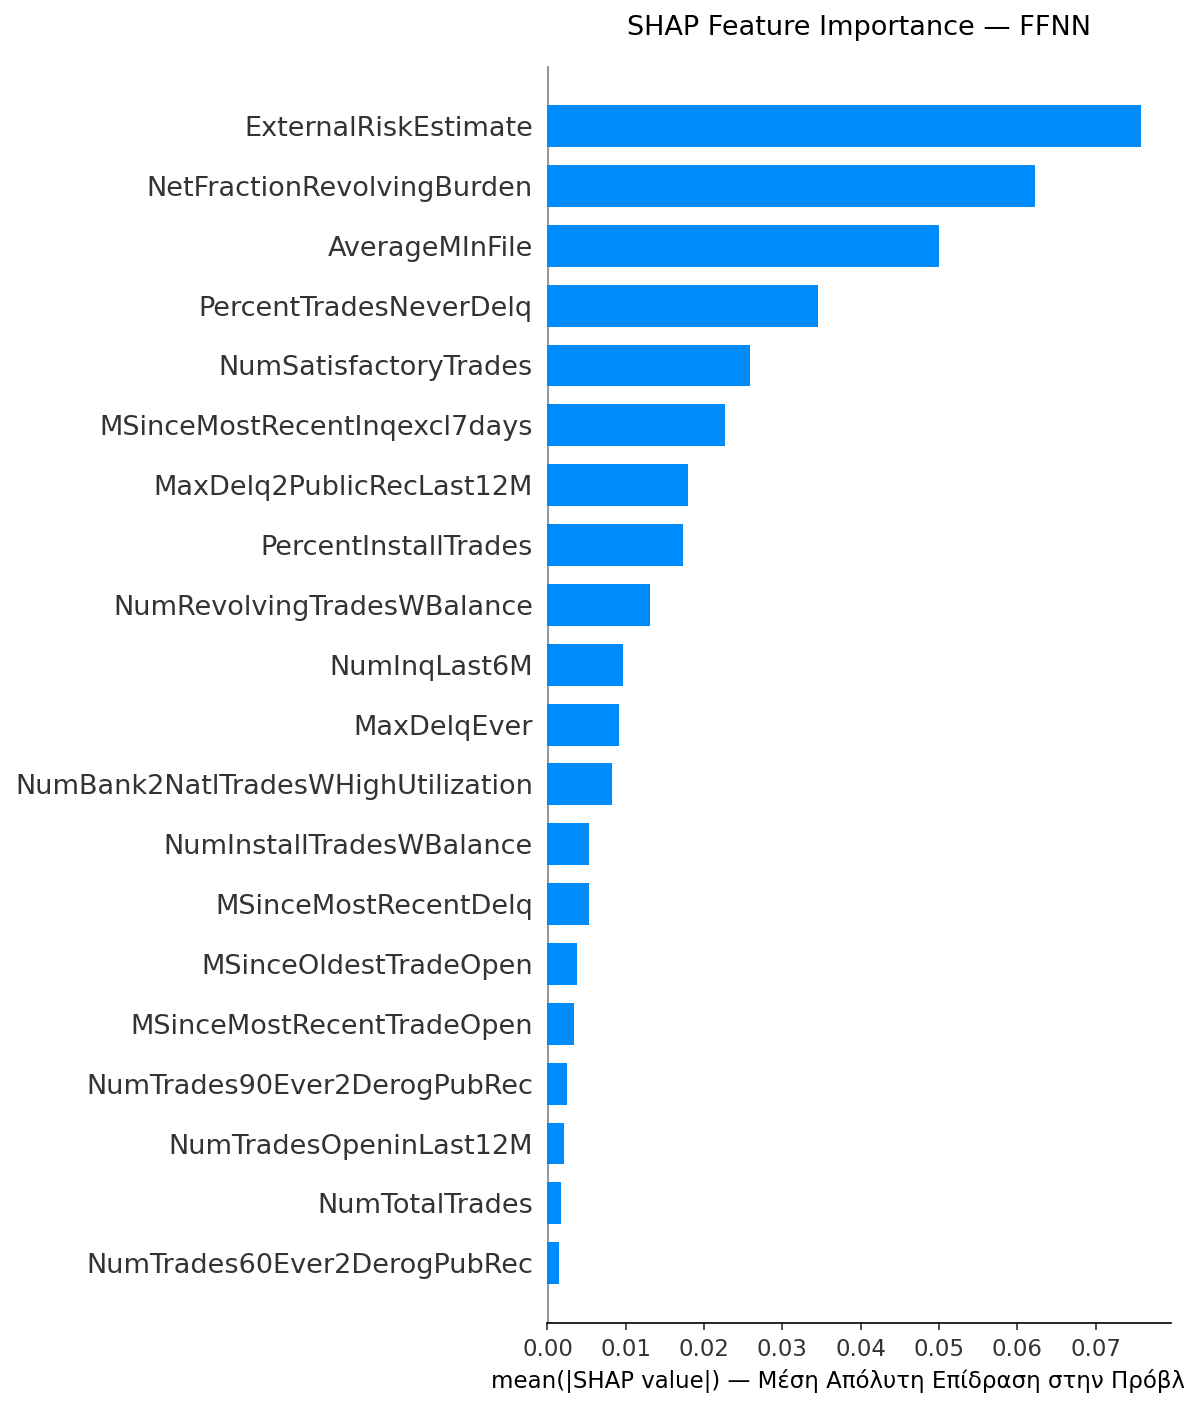
\includegraphics[width=0.80\textwidth]{10_shap_ffnn_importance}
    \caption[SHAP Feature Importance — FFNN]{SHAP Feature Importance για το FFNN υπολογισμένο με
             KernelExplainer. Κορυφαίο χαρακτηριστικό το
             \texttt{ExternalRiskEstimate}, συνεπές με το αντίστοιχο
             αποτέλεσμα του XGBoost. Οι τιμές του άξονα x είναι μη
             συγκρίσιμες με αυτές του Σχήματος~\ref{fig:shap_importance}
             λόγω διαφορετικής κλίμακας εξόδου των δύο μοντέλων.}
    \label{fig:shap_ffnn_importance}
\end{figure}



% 11_shap_comparison.png
Το Σχήμα~\ref{fig:shap_comparison} συγκρίνει τα διαγράμματα SHAP importance
των δύο μοντέλων για τα 10 πιο σημαντικά χαρακτηριστικά του XGBoost
(Σχήμα~\ref{fig:shap_importance}).
Αξίζει να σημειωθεί ότι 8 από τα 10 αυτά χαρακτηριστικά ανήκουν επίσης
στα 10 σημαντικότερα του FFNN (Σχήμα~\ref{fig:shap_ffnn_importance}).
Εξαίρεση αποτελούν το \texttt{MaxDelq2PublicRecLast12M} και το
\texttt{NumInqLast6M}, τα οποία κατατάσσονται στη 12η και 14η θέση
αντίστοιχα για το XGBoost αλλά στην 7η και 10η για το FFNN οπότε
δεν εμφανίζονται στο αντίστοιχο panel του διαγράμματος.
Συμπερασματικά τα δύο μοντέλα παρουσιάζουν υψηλή συμφωνία ως προς τη σχετική
βαρύτητα των χαρακτηριστικών.

% -------------------------------------------------------------------
% Σχήμα 4.13 — SHAP Comparison XGBoost vs FFNN (NB03)
% Τοποθέτηση: αμέσως μετά το κείμενο ανάλυσης
% -------------------------------------------------------------------
\begin{figure}[htbp]
    \centering
    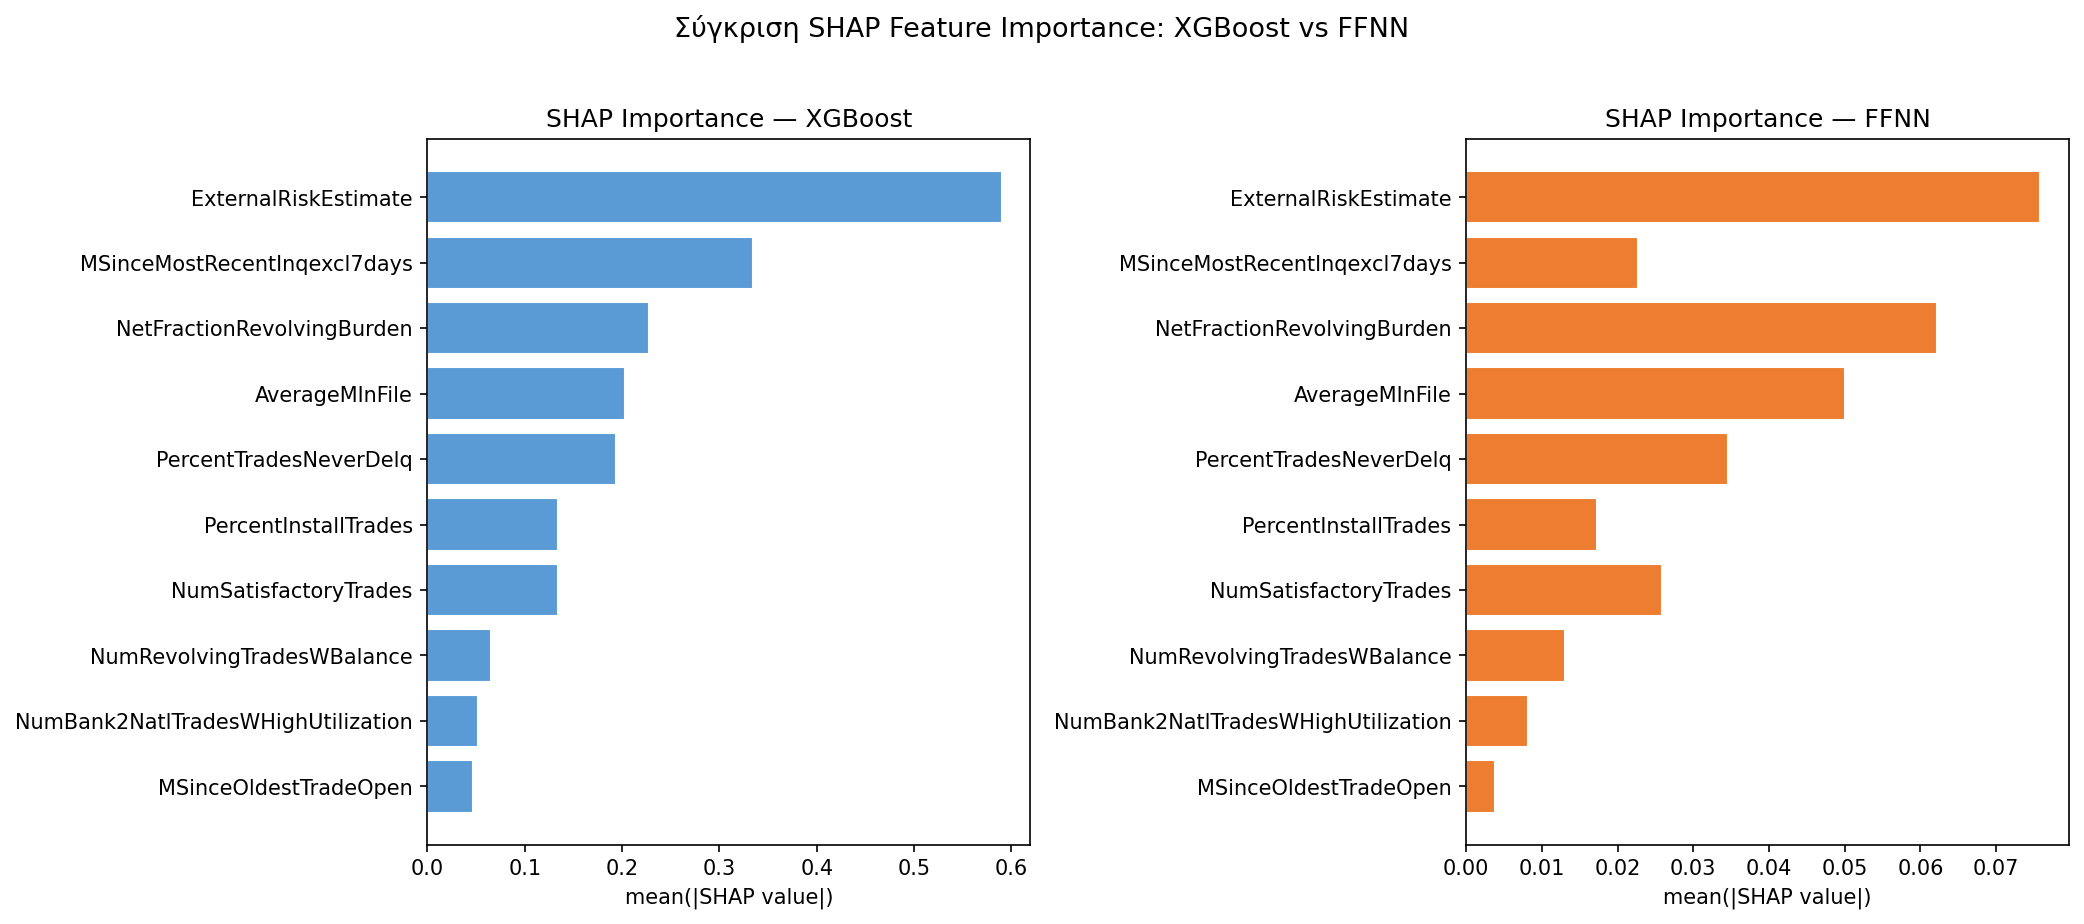
\includegraphics[width=\textwidth]{11_shap_comparison}
    \caption[Σύγκριση SHAP XGBoost vs FFNN]{Σύγκριση SHAP Feature Importance XGBoost και FFNN για τα
             10 σημαντικότερα χαρακτηριστικά του XGBoost.Οι δύο άξονες 
             x έχουν διαφορετική κλίμακα λόγω της διαφορετικής
            κλίμακας εξόδου των δύο μοντέλων --- η σύγκριση αφορά τη σχετική
            κατάταξη των χαρακτηριστικών, όχι τα απόλυτα μεγέθη.}
    \label{fig:shap_comparison}
\end{figure}




% 24_kernelexplainer_convergence.png
Το Σχήμα~\ref{fig:kernelexplainer_convergence} παρουσιάζει τα αποτελέσματα
του KernelExplainer για δύο προσεγγίσεις, μικρής και μέτριας υπολογιστικής
απαίτησης, και για την πλήρη ανάλυση.
Στην αριστερή πλευρά υπάρχει το διάγραμμα κανονικοποιημένης σημαντικότητας
των 10 σημαντικότερων χαρακτηριστικών του FFNN.
Στη δεξιά πλευρά εμφανίζεται το διάγραμμα κατάταξης συσχέτισης Spearman
για τις δύο προσεγγίσεις.

Στο διάγραμμα κανονικοποιημένης σημαντικότητας παρατηρείται ότι ενώ οι
τιμές των δύο προσεγγίσεων δεν διαφέρουν σημαντικά από αυτές της πλήρους
ανάλυσης, η διαφορά τους θα είχε ως αποτέλεσμα τη διαφορετική κατάταξη
σημαντικότητας των μεταβλητών.
Συγκεκριμένα, για τη μεταβλητή \texttt{NumSatisfactoryTrades} η μικρότερη
υπολογιστικά προσέγγιση έχει αποδώσει μικρότερη σημαντικότητα από την
\texttt{MSinceMostRecentInqexcl7days}, ενώ στην πλήρη ανάλυση το
\texttt{NumSatisfactoryTrades} προηγείται στην κατάταξη.
Παρόμοια παρατήρηση γίνεται για τις μεταβλητές \texttt{PercentInstallTrades}
και \texttt{NumRevolvingTradesWBalance} για τη μεγαλύτερη υπολογιστικά
προσέγγιση.
Οι παρατηρήσεις αυτές υπογραμμίζουν το γεγονός ότι χωρίς την πλήρη
ανάλυση, η οποία είναι δυσανάλογα απαιτητική σε υπολογιστικούς πόρους,
δεν μπορούμε να είμαστε σίγουροι για τα αποτελέσματα.

Στο διάγραμμα κατάταξης συσχέτισης Spearman παρατηρούμε ότι και οι δύο
προσεγγίσεις ξεπερνούν τόσο το όριο $0{,}90$ της αποδεκτής συσχέτισης
όσο και το όριο υψηλής συσχέτισης που είναι ίσο με $0{,}95$.
Οι τιμές τους $0{,}986$ και $0{,}992$ είναι αρκετά υψηλές και αποδεικνύουν
μια ακριβή προσέγγιση του αποτελέσματος της πλήρους ανάλυσης.
Παρά την διαφορά στην κατάταξη των χαρακτηριστικών, συνολικά τα
αποτελέσματα δεν διαφέρουν σημαντικά.
Εμπειρικά αποδεικνύεται ότι για το παρόν μοντέλο και βάση δεδομένων θα
μπορούσε να γίνει μια από τις δύο προσεγγίσεις εξοικονομώντας αρκετό
χρόνο, εφόσον οι προσεγγίσεις είναι της τάξης των μερικών λεπτών ενώ η
πλήρης προσέγγιση χρειάζεται $2{,}5$ ώρες.
Το αποτέλεσμα αυτό δεν μπορεί να γενικευτεί για άλλες βάσεις δεδομένων
και μοντέλα, καθώς χωρίς την πλήρη ανάλυση δεν γίνεται να είμαστε
σίγουροι για τον ρυθμό σύγκλισης των προσεγγίσεων.
Τέλος, αξίζει να αναφερθεί η σημαντική διαφορά της υπολογιστικής
απαίτησης ανάμεσα στα μοντέλα XGBoost και FFNN, δηλαδή ανάμεσα στις
συναρτήσεις TreeExplainer και KernelExplainer.
Η πλήρης ανάλυση του TreeExplainer διαρκεί μόλις λίγα δευτερόλεπτα σε
αντίθεση με τις $2{,}5$ ώρες για τον KernelExplainer.
Η ανάλυση για το μοντέλο XGBoost είναι τάξεις μικρότερη, έτσι ώστε
ακόμα και η διαφορά της με τις προσεγγίσεις των 2 και 10 λεπτών να
είναι εμφανής.
Η διαφορά αυτή προφανώς αυξάνεται και γίνεται δυσκολότερα διαχειρίσιμη
για μεγαλύτερες βάσεις δεδομένων.

% -------------------------------------------------------------------
% Σχήμα 4.14 — KernelExplainer Convergence (NB03)
% Τοποθέτηση: αμέσως μετά το κείμενο ανάλυσης
% -------------------------------------------------------------------
\begin{figure}[htbp]
    \centering
    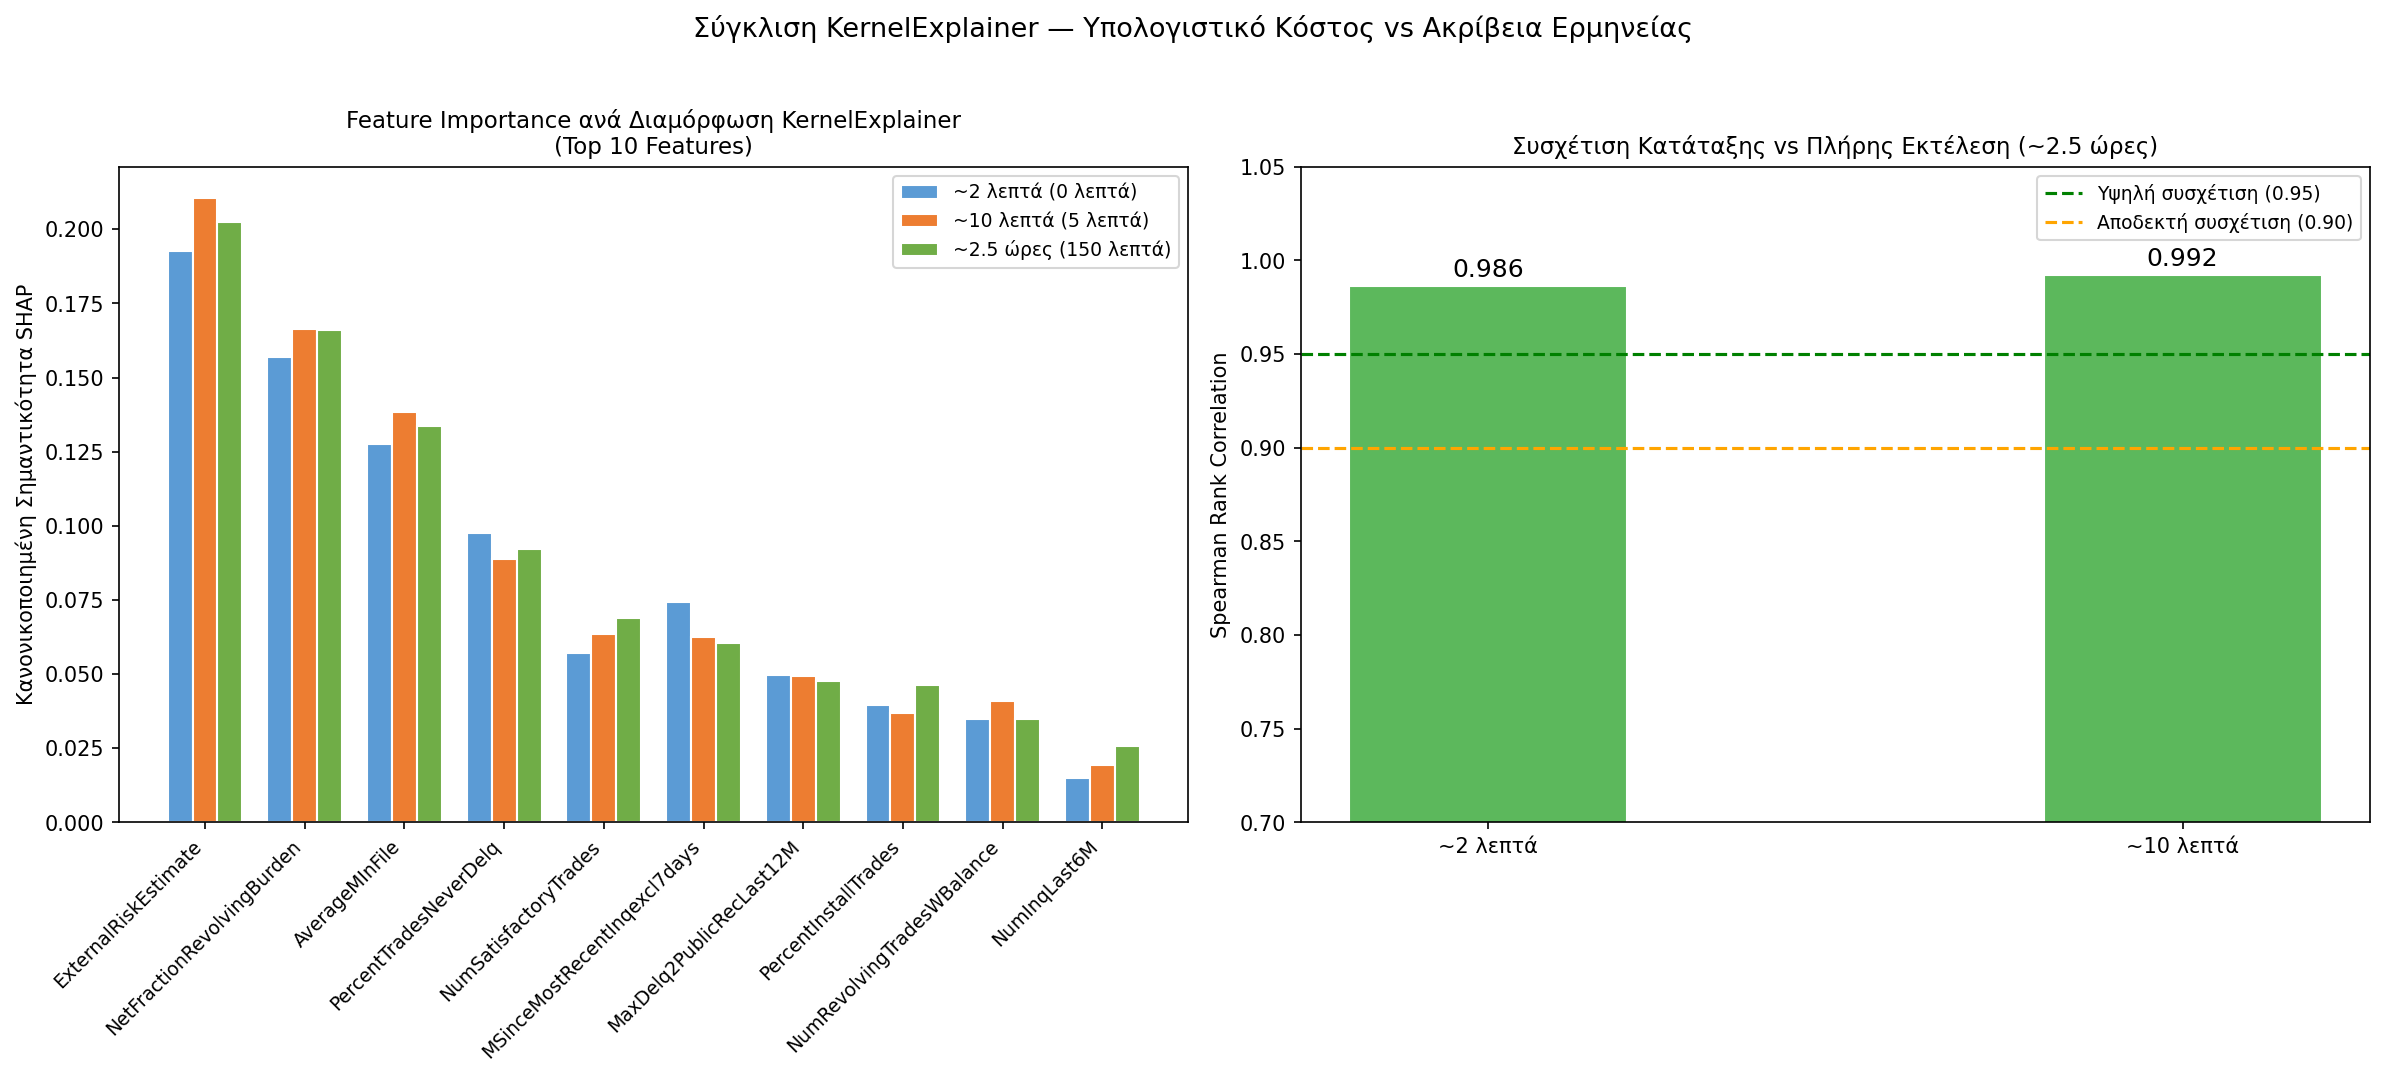
\includegraphics[width=\textwidth]{24_kernelexplainer_convergence}
    \caption[Σύγκλιση KernelExplainer — FFNN]{Σύγκλιση KernelExplainer για το FFNN. Αριστερά: κανονικοποιημένη
             σημαντικότητα SHAP για τρεις διαμορφώσεις (${\sim}2$ λεπτά,
             ${\sim}10$ λεπτά, ${\sim}2{,}5$ ώρες). Δεξιά: Spearman rank
             correlation κάθε προσέγγισης έναντι της πλήρους ανάλυσης.
             Και οι δύο προσεγγίσεις ξεπερνούν το όριο υψηλής συσχέτισης
             $0{,}95$, αποδεικνύοντας εμπειρικά αποδεκτή σύγκλιση για
             το παρόν dataset.}
    \label{fig:kernelexplainer_convergence}
\end{figure}

%==============================================================
\section{Ανίχνευση και Μετριασμός Μεροληψίας}
\label{sec:results_bias}

\subsection{Ανίχνευση Μεροληψίας}
\label{subsec:bias_detection}

Η ανίχνευση μεροληψίας πραγματοποιήθηκε και στα τρία μοντέλα με τις μετρικές
Δημογραφικής Ισότητας (DPD) και Ανισομερούς Επίπτωσης (DI) που περιεγράφηκαν
στην ενότητα~\ref{sec:bias_methodology}. Οι δανειολήπτες χωρίστηκαν στις ομάδες Α και Β
ανάλογα με την τιμή του χαρακτηριστικού \texttt{AverageMInFile} το οποίο
συμβολίζει την παλαιότητα του πιστωτικού τους ιστορικού. Η Ομάδα Α αντιστοιχεί
σε \texttt{AverageMInFile} κάτω της διαμέσου (76 μήνες) (βραχύ πιστωτικό
ιστορικό) και η Ομάδα Β σε τιμές πάνω της διαμέσου (παλαιό πιστωτικό ιστορικό). Ο διαχωρισμός βάση της διαμέσου 
επιτρέπει τη δημιουργία ομάδων ίσου μεγέθους διασφαλίζοντας έτσι τη στατιστική αξιοπιστία των group fairness metrics \citep{barocas2019fairness}.
Η επιλογή της συγκεκριμένης μεταβλητής εξηγήθηκε αναλυτικά στην
ενότητα~\ref{sec:bias_methodology}.

Ο Πίνακας~\ref{tab:bias_results} περιέχει τα ποσοστά έγκρισης της κάθε ομάδας
καθώς και τους δείκτες DPD και DI που υπολογίζονται από αυτά για τα τρία μοντέλα.
Το ιδανικό αποτέλεσμα θα ήταν οι δύο ομάδες να έχουν παρόμοια ποσοστά έγκρισης
και δείκτες DPD κάτω του 0{,}1 και DI άνω του 0{,}8. Τέτοιο αποτέλεσμα δεν
παρατηρείται σε κανένα μοντέλο. Και οι τρεις αλγόριθμοι έχουν σχεδόν ίδια
ποσοστά έγκρισης, 30\% για την Α και 62\% για την Β, ενώ οι διαφορές στους
δύο δείκτες είναι αμελητέες. Στον δείκτη DPD τα μοντέλα έχουν βαθμολογία
${\sim}0{,}33$ και στον DI ${\sim}0{,}47$, και οι δύο πολύ μακριά των αποδεκτών
ορίων. Παρατηρείται λοιπόν μεροληψία και στους τρεις αλγορίθμους υπέρ των
δανειοληπτών της Ομάδας Β.

% -------------------------------------------------------------------
% Πίνακας 4.3 — Bias Detection αποτελέσματα
% Τοποθέτηση: αμέσως μετά την πρώτη παράγραφο
% -------------------------------------------------------------------
\begin{table}[htbp]
    \centering
    \caption[Αποτελέσματα ανίχνευσης μεροληψίας]{Αποτελέσματα ανίχνευσης μεροληψίας για τα τρία μοντέλα.
    Όριο αποδοχής: DPD $< 0{,}10$, DI $\geq 0{,}80$.}
    \label{tab:bias_results}
    \begin{tabular}{lcccc}
        \toprule
        \textbf{Μοντέλο} & \textbf{Ομάδα Α} & \textbf{Ομάδα Β}
        & \textbf{DPD} & \textbf{DI} \\
        \midrule
        Logistic Regression & 30{,}1\% & 63{,}9\% & 0{,}3381 & 0{,}4712 \\
        XGBoost             & 29{,}6\% & 62{,}4\% & 0{,}3287 & 0{,}4737 \\
        FFNN                & 30{,}4\% & 62{,}7\% & 0{,}3233 & 0{,}4846 \\
        \bottomrule
    \end{tabular}
\end{table}

Το Σχήμα~\ref{fig:bias_comparison} παρουσιάζει οπτικά τα αποτελέσματα του
Πίνακα~\ref{tab:bias_results}. Το γεγονός ότι και τα τρία μοντέλα εμφανίζουν
παρόμοια στατιστικά και βαθμολογία στους δείκτες μας οδηγεί στο συμπέρασμα
ότι η μεροληψία δημιουργείται από την βάση δεδομένων \citep{mehrabi2021survey, suresh2021framework}. 
Η εμφάνιση μεροληψίας
στην συγκεκριμένη προσομοίωση δεν υποδεικνύει λάθος στην «εσωτερική λογική»
κάποιου μοντέλου καθώς όλα τους παράγουν ίδια αποτελέσματα. Η μόνη λογική
εξήγηση είναι ότι η βάση δεδομένων περιέχει δεδομένα πιστωτικού κίνδυνου τα
οποία ευνοούν τους δανειολήπτες με μακρύ πιστωτικό ιστορικό. Το γεγονός αυτό
δεν καθιστά προβληματική την βάση καθώς το συγκεκριμένο χαρακτηριστικό μπορεί
να έχει πραγματικό αντίκτυπο στην πιθανότητα αθέτησης του δανείου. Επιπλέον,
υπάρχει η πιθανότητα η βάση δεδομένων να μην είναι αντιπροσωπευτική και τελικά
αυτός να είναι ο λόγος που παράγει μεροληψία. Και στις δύο περιπτώσεις οι
ρυθμιστικές αρχές απαιτούν έλεγχο και αντιμετώπιση της μεροληψίας \citep{eba2023} ακόμα και
εάν είναι εις βάρος της απόδοσης των μοντέλων.

% -------------------------------------------------------------------
% Σχήμα 4.15 — Bias Comparison τριών μοντέλων (NB04)
% Τοποθέτηση: αμέσως μετά την τελευταία παράγραφο
% -------------------------------------------------------------------
\begin{figure}[htbp]
    \centering
    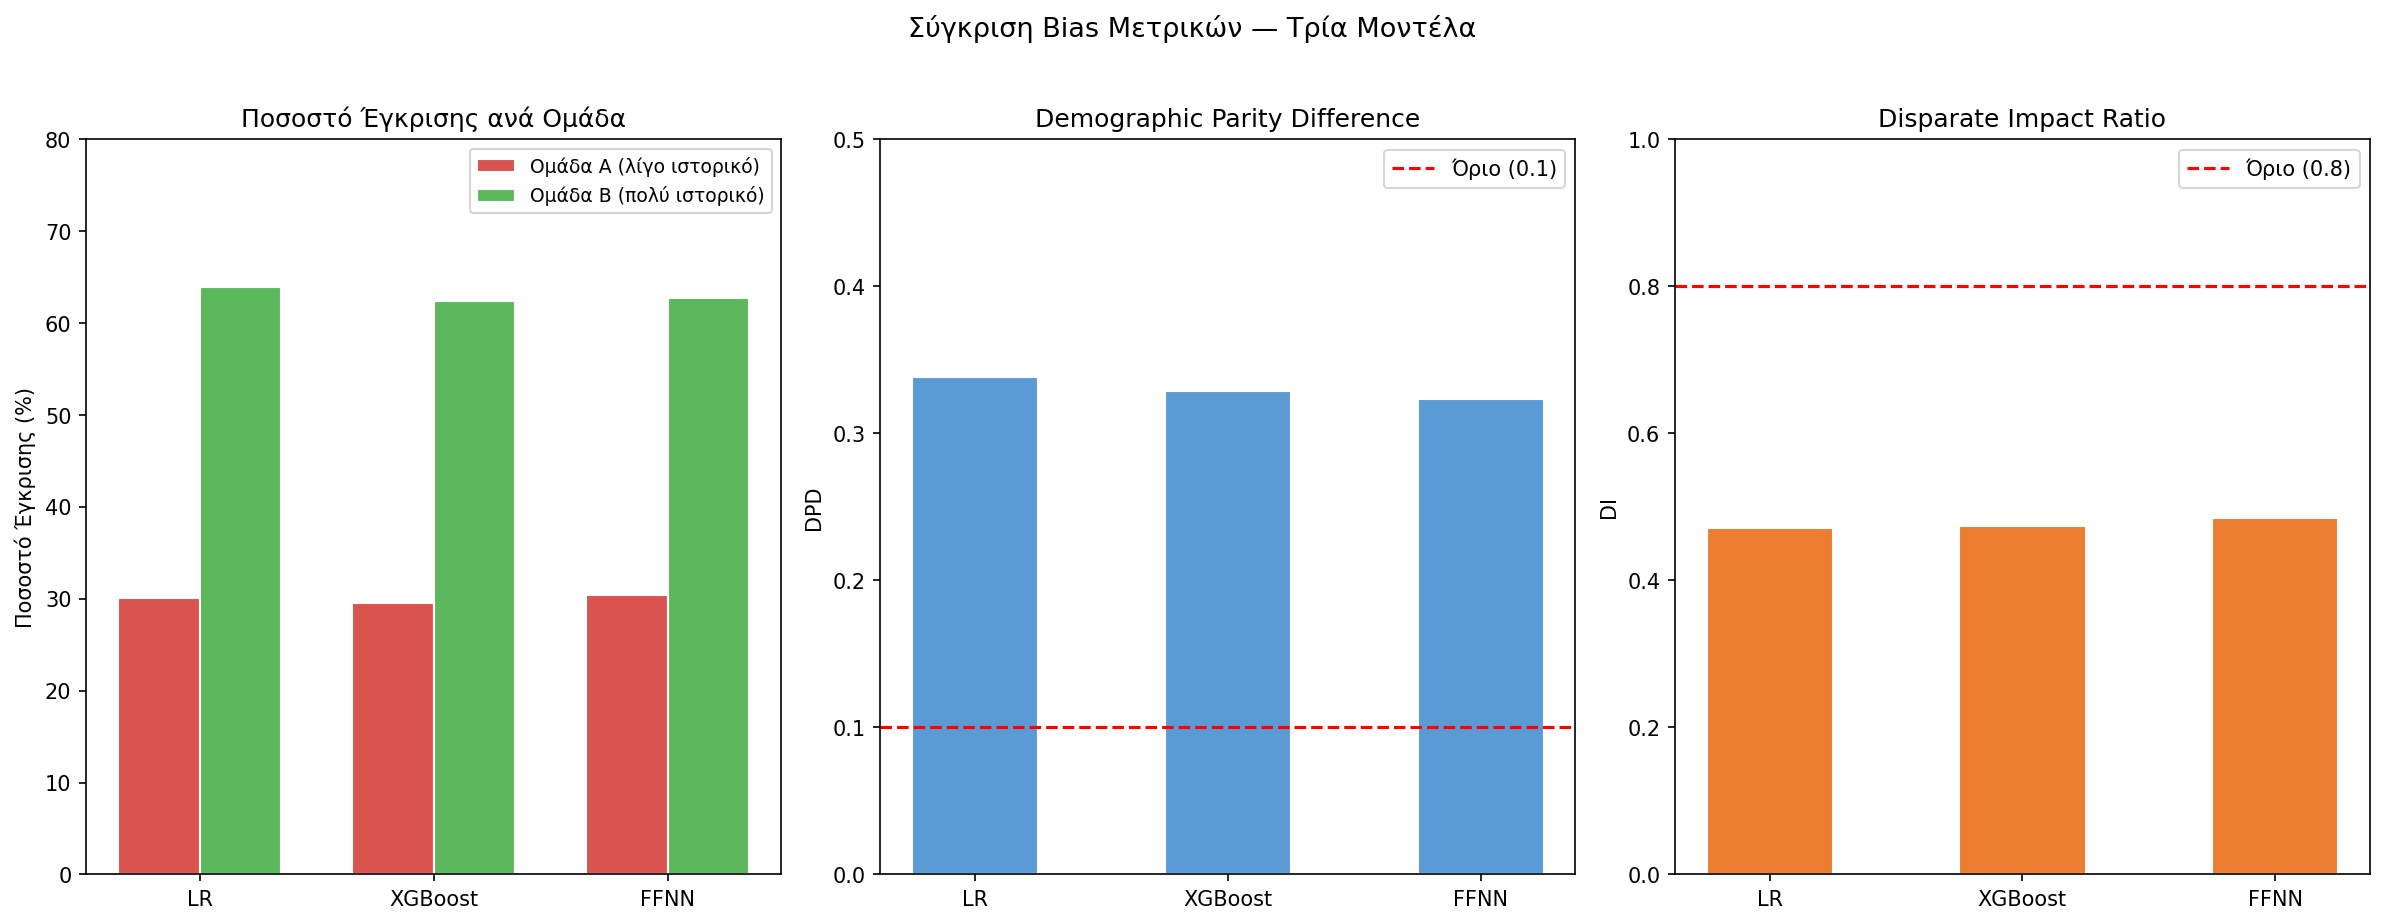
\includegraphics[width=\textwidth]{12_bias_comparison}
    \caption[Σύγκριση μετρικών μεροληψίας τριών μοντέλων]{Σύγκριση μετρικών μεροληψίας για τα τρία μοντέλα. Αριστερά:
             ποσοστά έγκρισης Ομάδας Α (βραχύ ιστορικό) και Ομάδας Β
             (παλαιό ιστορικό). Κέντρο: Demographic Parity Difference ---
             η διακεκομμένη γραμμή δείχνει το όριο $0{,}10$. Δεξιά:
             Disparate Impact Ratio --- η διακεκομμένη γραμμή δείχνει
             το όριο $0{,}80$. Και τα τρία μοντέλα εμφανίζουν DI
             ${\sim}0{,}47$, σημαντικά κάτω του αποδεκτού ορίου.}
    \label{fig:bias_comparison}
\end{figure}


\subsection{Μετριασμός Μεροληψίας}
\label{subsec:bias_mitigation}

Για την επίδειξη της τεχνικής μετριασμού εφαρμόστηκε ο αλγόριθμος
\texttt{ExponentiatedGradient} της βιβλιοθήκης Fairlearn με base estimator τη
Logistic Regression και ο χειροκίνητος ThresholdOptimizer μέσω grid search
για το XGBoost, για τους λόγους που αναφέρθηκαν στην
ενότητα~\ref{sec:bias_methodology}.

Στο Σχήμα~\ref{fig:fairness_mitigation} παρουσιάζονται τα αποτελέσματα για την
Logistic Regression. Στο αριστερό μέρος το διάγραμμα για την μετρική DI πριν
και μετά την διαδικασία συμμόρφωσης αποδεικνύει ότι άλλαξε η συμπεριφορά του
μοντέλου πετυχαίνοντας απόδοση $0{,}931$ από $0{,}471$, μεγαλύτερη του ορίου
$0{,}8$. Στο δεξί μέρος του σχήματος το διάγραμμα της μετρικής AUC
οπτικοποιεί τις επιπτώσεις του mitigation στην απόδοση. Το κόστος του Fairness
mitigation φαίνεται να είναι μια σχετική μείωση της τάξης του 14\% στην AUC
καθώς η βαθμολογία του αλγορίθμου μειώθηκε από $0{,}789$ σε $0{,}680$.

% -------------------------------------------------------------------
% Σχήμα 4.16 — Fairness Mitigation LR (NB04)
% Τοποθέτηση: αμέσως μετά την παράγραφο LR
% -------------------------------------------------------------------
\begin{figure}[htbp]
    \centering
    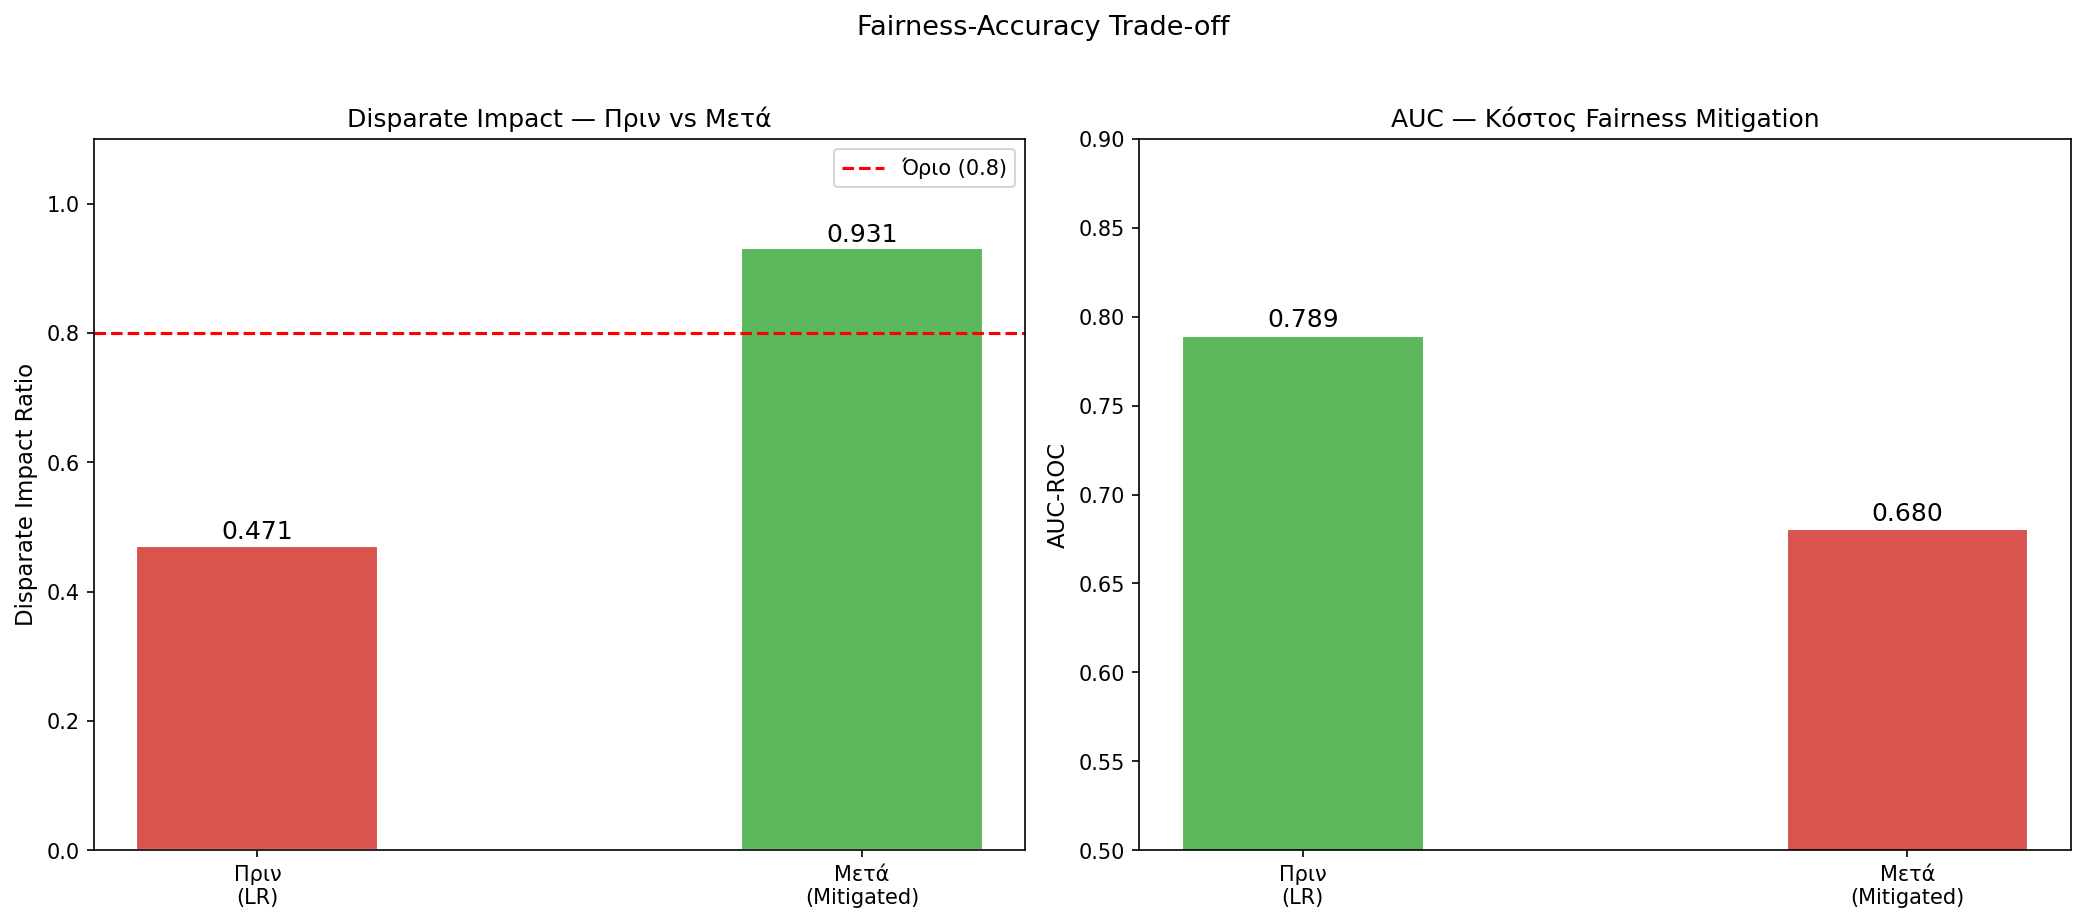
\includegraphics[width=\textwidth]{20_fairness_mitigation}
    \caption[Fairness mitigation — Logistic Regression]{Αποτελέσματα fairness mitigation για την Logistic Regression
             με \texttt{ExponentiatedGradient}. Αριστερά: DI πριν
             ($0{,}471$) και μετά ($0{,}931$) --- η διακεκομμένη γραμμή
             δείχνει το όριο $0{,}80$. Δεξιά: AUC πριν ($0{,}789$) και
             μετά ($0{,}680$) --- κόστος $0{,}109$ μονάδων.}
    \label{fig:fairness_mitigation}
\end{figure}

Στο Σχήμα~\ref{fig:fairness_mitigation_comparison} συγκρίνονται τα αποτελέσματα
του μοντέλου LR με το XGBoost. Στο αριστερό μέρος, στο διάγραμμα για την
μετρική DI παρατηρείται ότι ο αλγόριθμος XGBoost καταφέρνει τέλεια βαθμολογία
$1{,}000$. Το ίδιο δεν συμβαίνει για τον αλγόριθμο LR διότι γίνεται αυτόματα
με την συνάρτηση \texttt{ExponentiatedGradient} με $\varepsilon = 0{,}01$ η
οποία προσεγγίζει το όριο χωρίς να το εγγυάται. Αξίζει να σημειωθεί ότι για
το XGBoost δεν έγιναν in-processing αλλαγές, δηλαδή επανεκπαίδευση μοντέλου,
αλλά post-processing αλλαγές στο κατώφλι πιθανότητας. Ως αποτέλεσμα η μετρική
AUC παραμένει αμετάβλητη και ίση με $0{,}796$. Όπως είδαμε στο
Σχήμα~\ref{fig:fairness_mitigation} το ίδιο δεν ισχύει για την LR. Τέλος, στο
δεξί μέρος το διάγραμμα Balanced Accuracy παρουσιάζει το κόστος της διαδικασίας
μετριασμού στα δύο μοντέλα. Παρόλο που η μετρική AUC παρέμεινε σταθερή υπάρχει
υπολογίσιμο κόστος και για το μοντέλο XGBoost. Τα αποτελέσματα δίνουν ξεκάθαρο
πλεονέκτημα στο μοντέλο XGBoost διότι κατάφερε τέλεια βαθμολόγηση στην μετρική
DI ενώ δεν χρειάστηκε επανεκπαίδευση η οποία απαιτεί περισσότερους
υπολογιστικούς πόρους.

% -------------------------------------------------------------------
% Σχήμα 4.17 — Fairness Mitigation Comparison LR vs XGBoost (NB04)
% Τοποθέτηση: αμέσως μετά την παράγραφο σύγκρισης
% -------------------------------------------------------------------
\begin{figure}[htbp]
    \centering
    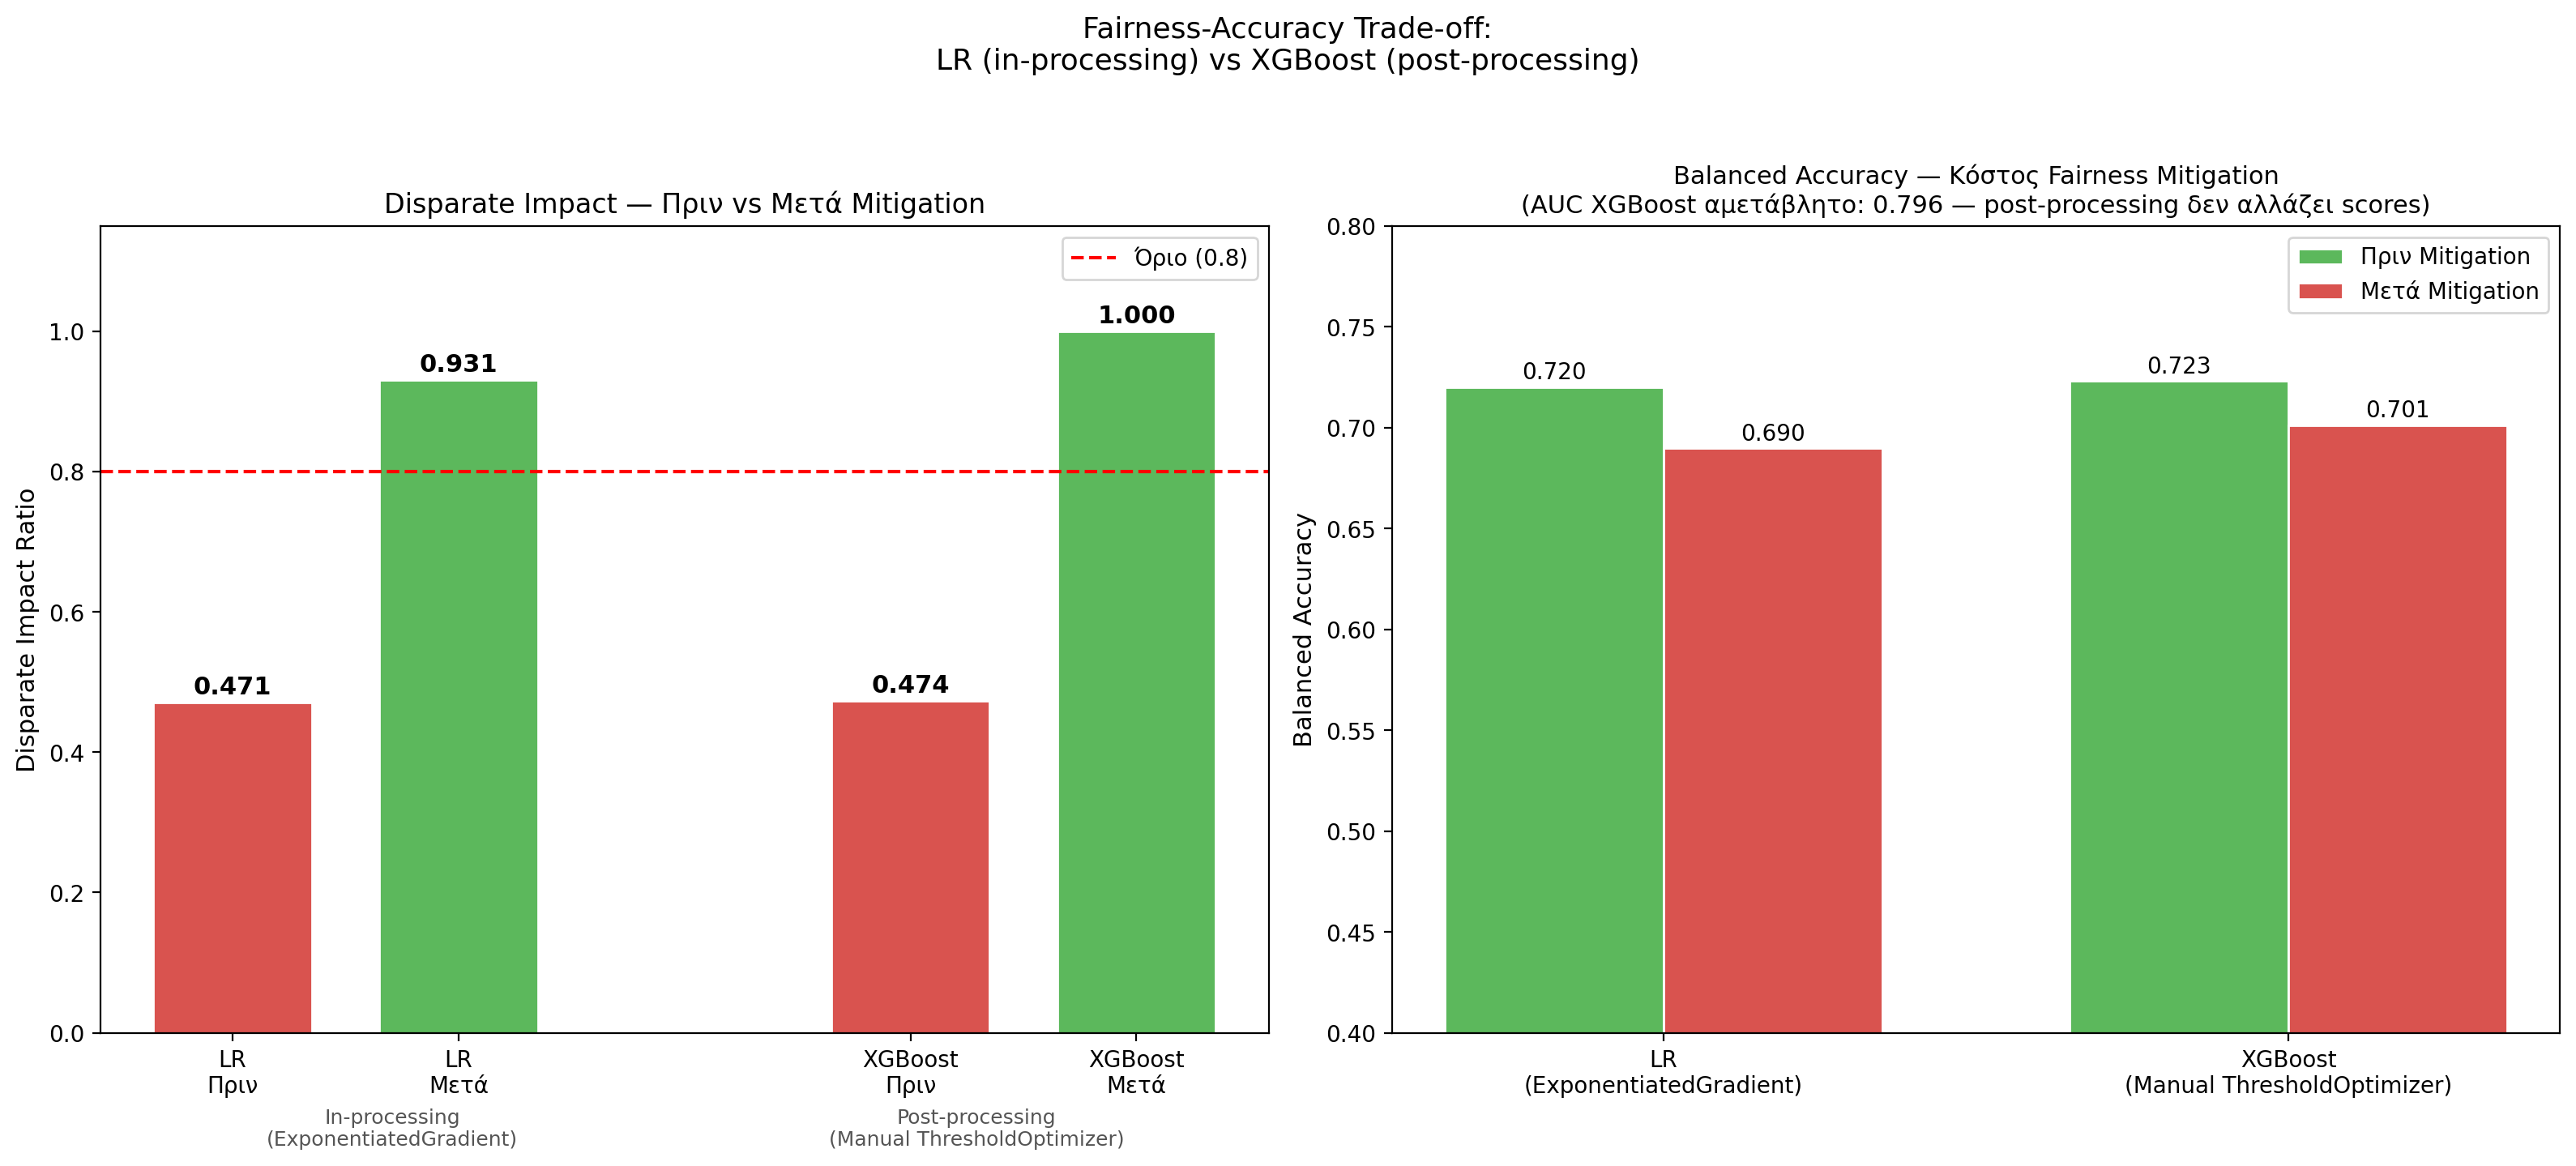
\includegraphics[width=\textwidth]{25_fairness_mitigation_comparison}
    \caption[Σύγκριση fairness mitigation LR vs XGBoost]{Σύγκριση fairness mitigation LR (in-processing,
             \texttt{ExponentiatedGradient}) και XGBoost (post-processing,
             Manual ThresholdOptimizer). Αριστερά: DI πριν και μετά για
             κάθε μοντέλο --- το XGBoost επιτυγχάνει DI $= 1{,}000$.
             Δεξιά: Balanced Accuracy πριν και μετά --- το AUC του
             XGBoost παραμένει αμετάβλητο στο $0{,}796$.}
    \label{fig:fairness_mitigation_comparison}
\end{figure}

Το παρατηρούμενο fairness-accuracy trade-off, όπως και η σχετικά καλύτερη 
συμπεριφορά του post-processing έναντι του in-processing, ευθυγραμμίζονται 
με τα εμπειρικά ευρήματα της βιβλιογραφίας στο fair credit scoring 
\citep{kozodoi2022fairness}.

%==============================================================
\section{Παρακολούθηση Σταθερότητας}
\label{sec:results_monitoring}
\subsection{Σταθερότητα Πληθυσμού --- PSI}
\label{subsec:results_psi}

% 17_psi_scenarios.png
Ο δείκτης PSI υπολογίστηκε για τα τρία σενάρια οικονομικής επιδείνωσης που
περιγράφηκαν στην ενότητα~\ref{sec:psi}. Τα αποτελέσματα για το XGBoost
παρουσιάζονται στο Σχήμα~\ref{fig:psi_scenarios}. Το σενάριο Βασικής Γραμμής
(Baseline) έχει $\text{PSI} = 0{,}000$. Για ήπια επιδείνωση υπολογίστηκε PSI
ίσο με $0{,}069$, που βρίσκεται κάτω από το όριο $0{,}10$ οπότε θεωρείται
σταθερό. Για μέτρια επιδείνωση το PSI είναι ίσο με $0{,}210$, βρίσκεται
ανάμεσα στα όρια $0{,}10$ και $0{,}25$, που υποδηλώνει ανάγκη παρακολούθησης.
Για σοβαρή επιδείνωση $\text{PSI} = 0{,}641$, πολύ πάνω από το $0{,}25$ οπότε
απαιτείται επανεκπαίδευση μοντέλου.

Η μετάβαση μεταξύ των σεναρίων τονίζει την χρησιμότητα του δείκτη PSI.
Υποθέτοντας ότι η επιδείνωση της οικονομίας δεν είναι ακαριαία και έτσι το
μοντέλο θα περνούσε από όλα τα προηγούμενα στάδια πριν καταλήξει σε κάποια
κατάσταση, συμπεραίνουμε ότι μέσω του δείκτη θα λάβουμε μια προειδοποίηση
για την απόδοση του μοντέλου πριν αυτή υποβαθμιστεί αισθητά και οδηγήσει
σε λάθος αποφάσεις στον πιστωτικό κίνδυνο.

% -------------------------------------------------------------------
% Σχήμα 4.18 — PSI Scenarios XGBoost (NB05)
% Τοποθέτηση: αμέσως μετά το κείμενο ανάλυσης
% -------------------------------------------------------------------
\begin{figure}[htbp]
    \centering
    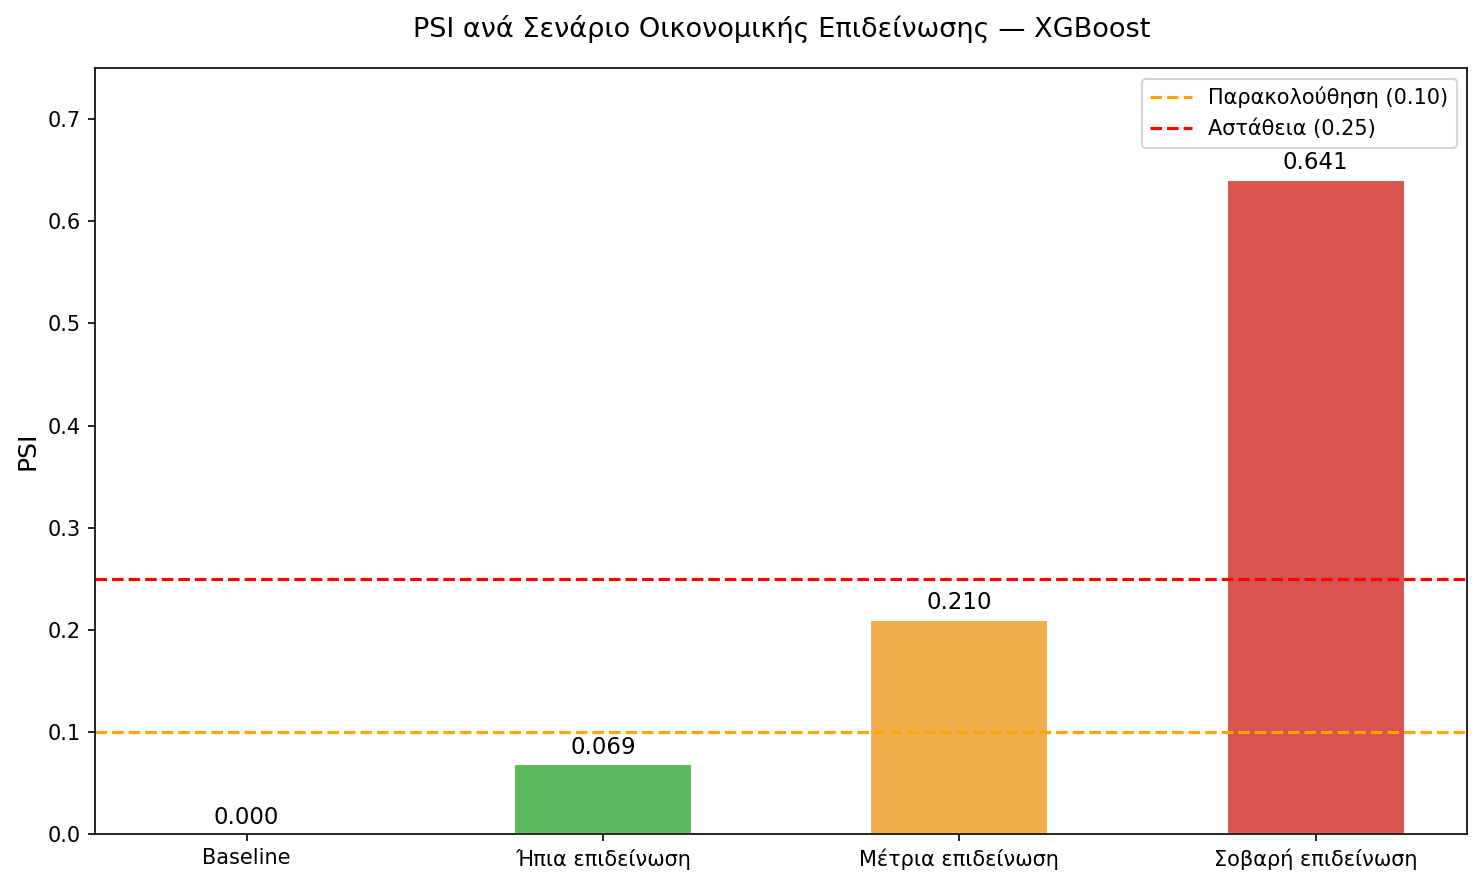
\includegraphics[width=\textwidth]{17_psi_scenarios}
    \caption[PSI σενάρια οικονομικής επιδείνωσης — XGBoost]{PSI για τέσσερα σενάρια οικονομικής επιδείνωσης (XGBoost).
             Χρωματική κωδικοποίηση: πράσινο $< 0{,}10$ (σταθερό),
             πορτοκαλί $0{,}10$--$0{,}25$ (παρακολούθηση),
             κόκκινο $> 0{,}25$ (επανεκπαίδευση).}
    \label{fig:psi_scenarios}
\end{figure}


\subsection{Σταθερότητα Χαρακτηριστικών — CSI}
\label{subsec:results_csi}
% 13_csi.png
Για κάθε χαρακτηριστικό της βάσης FICO HELOC υπολογίστηκε ο δείκτης CSI
στο σενάριο της μέτριας επιδείνωσης. Τα αποτελέσματα παρουσιάζονται στο
Σχήμα~\ref{fig:csi}. Όπως ήταν αναμενόμενο, τα τρία χαρακτηριστικά που
υπέστησαν τις μεγαλύτερες αλλαγές μέσω της προσομοίωσης εμφανίζονται με
κόκκινο χρώμα --- \texttt{ExternalRiskEstimate} και
\texttt{NetFractionRevolvingBurden} έχουν περάσει το όριο αστάθειας ---
και πορτοκαλί χρώμα το \texttt{AverageMInFile}, εφόσον βρίσκεται στην
περιοχή που δηλώνει ανάγκη παρακολούθησης.
Εκτός από τις τρεις αυτές μεταβλητές, στις υπόλοιπες έχει προστεθεί μόνο
λευκός θόρυβος ($0{,}1$ std) ο οποίος δεν προκαλεί σοβαρή μεταβολή στις
τιμές τους, με αποτέλεσμα ο δείκτης CSI τους να παραμένει κάτω από $0{,}10$.
Εξαίρεση αποτελούν τα χαρακτηριστικά \texttt{MaxDelq2PublicRecLast12M}
($\text{CSI} = 0{,}920$) και \texttt{MaxDelqEver} ($\text{CSI} = 0{,}906$),
τα οποία βρίσκονται πέραν του ορίου αστάθειας με τιμές μάλιστα υψηλότερες
από τα σκόπιμα τροποποιημένα χαρακτηριστικά. Η τεχνητά υψηλή τιμή τους
οφείλεται στη διακριτή φύση των τιμών τους και εξηγείται αναλυτικά στην
ενότητα~\ref{sec:csi}.

% -------------------------------------------------------------------
% Σχήμα 4.19 — CSI ανά χαρακτηριστικό (NB05)
% Τοποθέτηση: αμέσως μετά το κείμενο ανάλυσης
% -------------------------------------------------------------------
\begin{figure}[htbp]
    \centering
    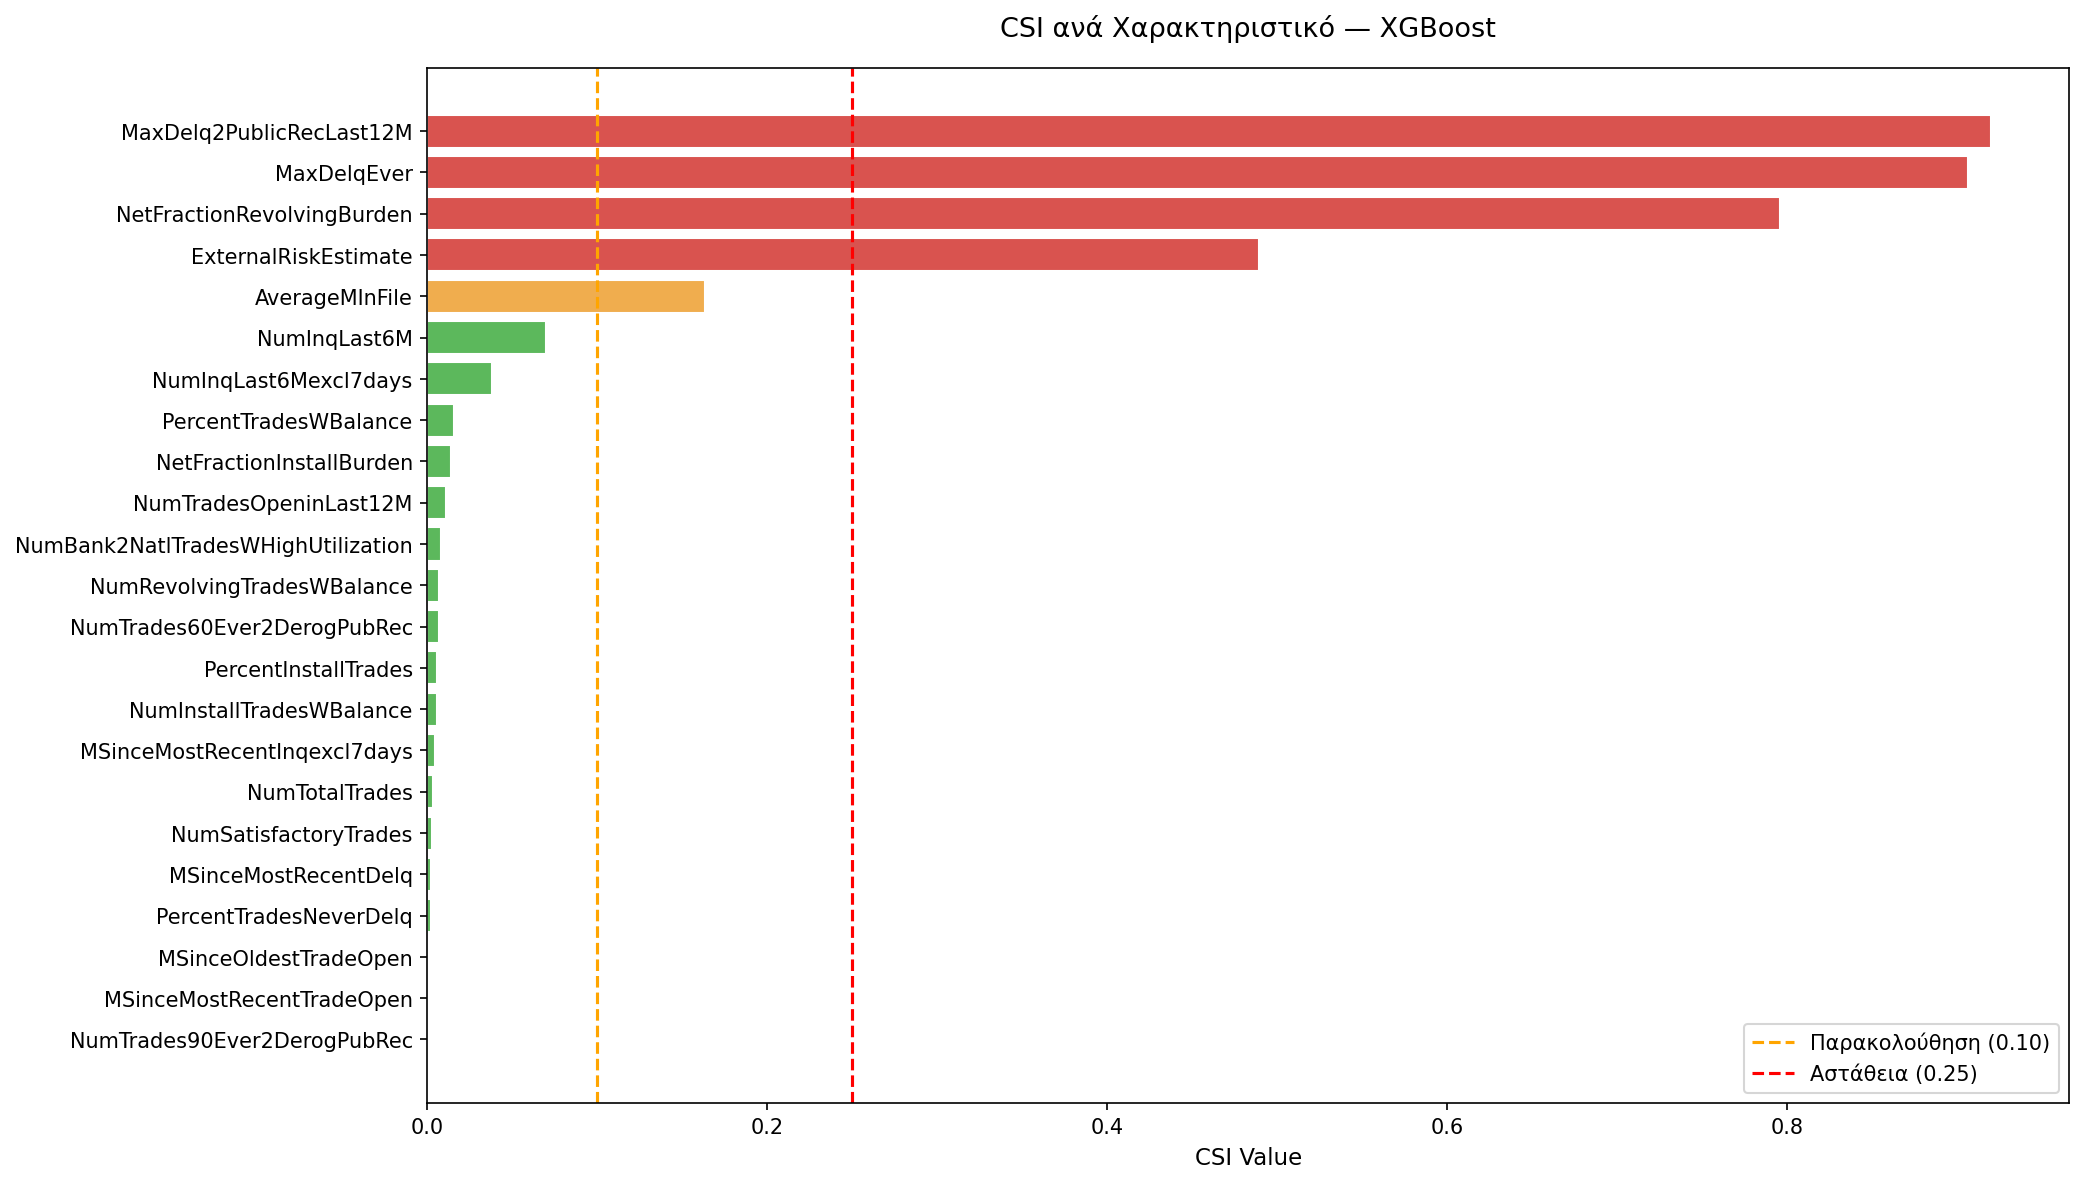
\includegraphics[width=\textwidth]{13_csi}
    \caption[CSI ανά χαρακτηριστικό — μέτρια επιδείνωση]{CSI για τα 23 χαρακτηριστικά της βάσης FICO HELOC στο σενάριο
             μέτριας επιδείνωσης. Χρωματική κωδικοποίηση: πράσινο $< 0{,}10$
             (σταθερό), πορτοκαλί $0{,}10$--$0{,}25$ (παρακολούθηση),
             κόκκινο $> 0{,}25$ (αστάθεια). Τα \texttt{MaxDelq2PublicRecLast12M}
             και \texttt{MaxDelqEver} εμφανίζουν τεχνητά υψηλό CSI λόγω
             διακριτής φύσης --- βλ.\ ενότητα~\ref{sec:csi}.}
    \label{fig:csi}
\end{figure}


\subsection{Σύγκριση Παρακολούθησης XGBoost και FFNN}
\label{subsec:results_monitoring_comparison}

% 21_monitoring_comparison.png
Στο Σχήμα~\ref{fig:monitoring_comparison} παρουσιάζεται η σύγκριση
παρακολούθησης για τα μοντέλα XGBoost και FFNN. Η δεξιά πλευρά του
σχήματος παρουσιάζει τα 10 πιο ασταθή χαρακτηριστικά σε ραβδοδιάγραμμα.
Οι τιμές CSI των χαρακτηριστικών είναι ίδιες και για τα δύο μοντέλα
καθώς εξαρτώνται μόνο από τις αλλαγές στα χαρακτηριστικά και όχι στην
πρόβλεψη του μοντέλου. Σε αντίθεση με τις τιμές CSI, τα αποτελέσματα
του δείκτη PSI εξαρτώνται από τις προβλέψεις των μοντέλων. Στο αριστερό
μέρος του σχήματος οπτικοποιούνται οι διαφορές για τους δύο αλγορίθμους.
Φαίνεται ότι και οι δύο αλγόριθμοι επηρεάζονται με τον ίδιο τρόπο από
τις αλλαγές, με τιμές PSI $0{,}036$ / $0{,}221$ / $0{,}653$ για το FFNN
έναντι $0{,}069$ / $0{,}210$ / $0{,}641$ για το XGBoost. Η μετρική PSI
προειδοποιεί επιτυχώς τόσο σε μέτρια όσο και σε σοβαρή επιδείνωση της
οικονομίας, ενώ δεν δίνει λανθασμένη ειδοποίηση σε περίπτωση ήπιας
αλλαγής. Παρά τη διαφορά στην πολυπλοκότητα των μοντέλων, η
παρακολούθησή τους με τους παραπάνω δείκτες δεν διαφέρει σημαντικά.
Η κρίσιμη διαφορά παραμένει στο κομμάτι της ερμηνείας, όπως
διαπιστώθηκε στην υποενότητα~\ref{sec:results_ffnn_shap}. Για το XGBoost,
εάν παρατηρηθεί σοβαρή αστάθεια μέσω της PSI, η συνάρτηση TreeExplainer
θα μπορέσει γρήγορα να εντοπίσει ποια χαρακτηριστικά την προκάλεσαν.
Σε αντίθεση με το XGBoost, το FFNN απαιτεί KernelExplainer, δηλαδή ώρες
υπολογισμού χωρίς εγγύηση ακρίβειας --- ένα απαγορευτικό γεγονός, διότι
ένα υψηλό CSI δεν θα μπορεί εύκολα να συνδεθεί με τις αλλαγές στο
αποτέλεσμα.

% -------------------------------------------------------------------
% Σχήμα 4.20 — Monitoring Comparison XGBoost vs FFNN (NB05)
% Τοποθέτηση: αμέσως μετά το κείμενο ανάλυσης
% -------------------------------------------------------------------
\begin{figure}[htbp]
    \centering
    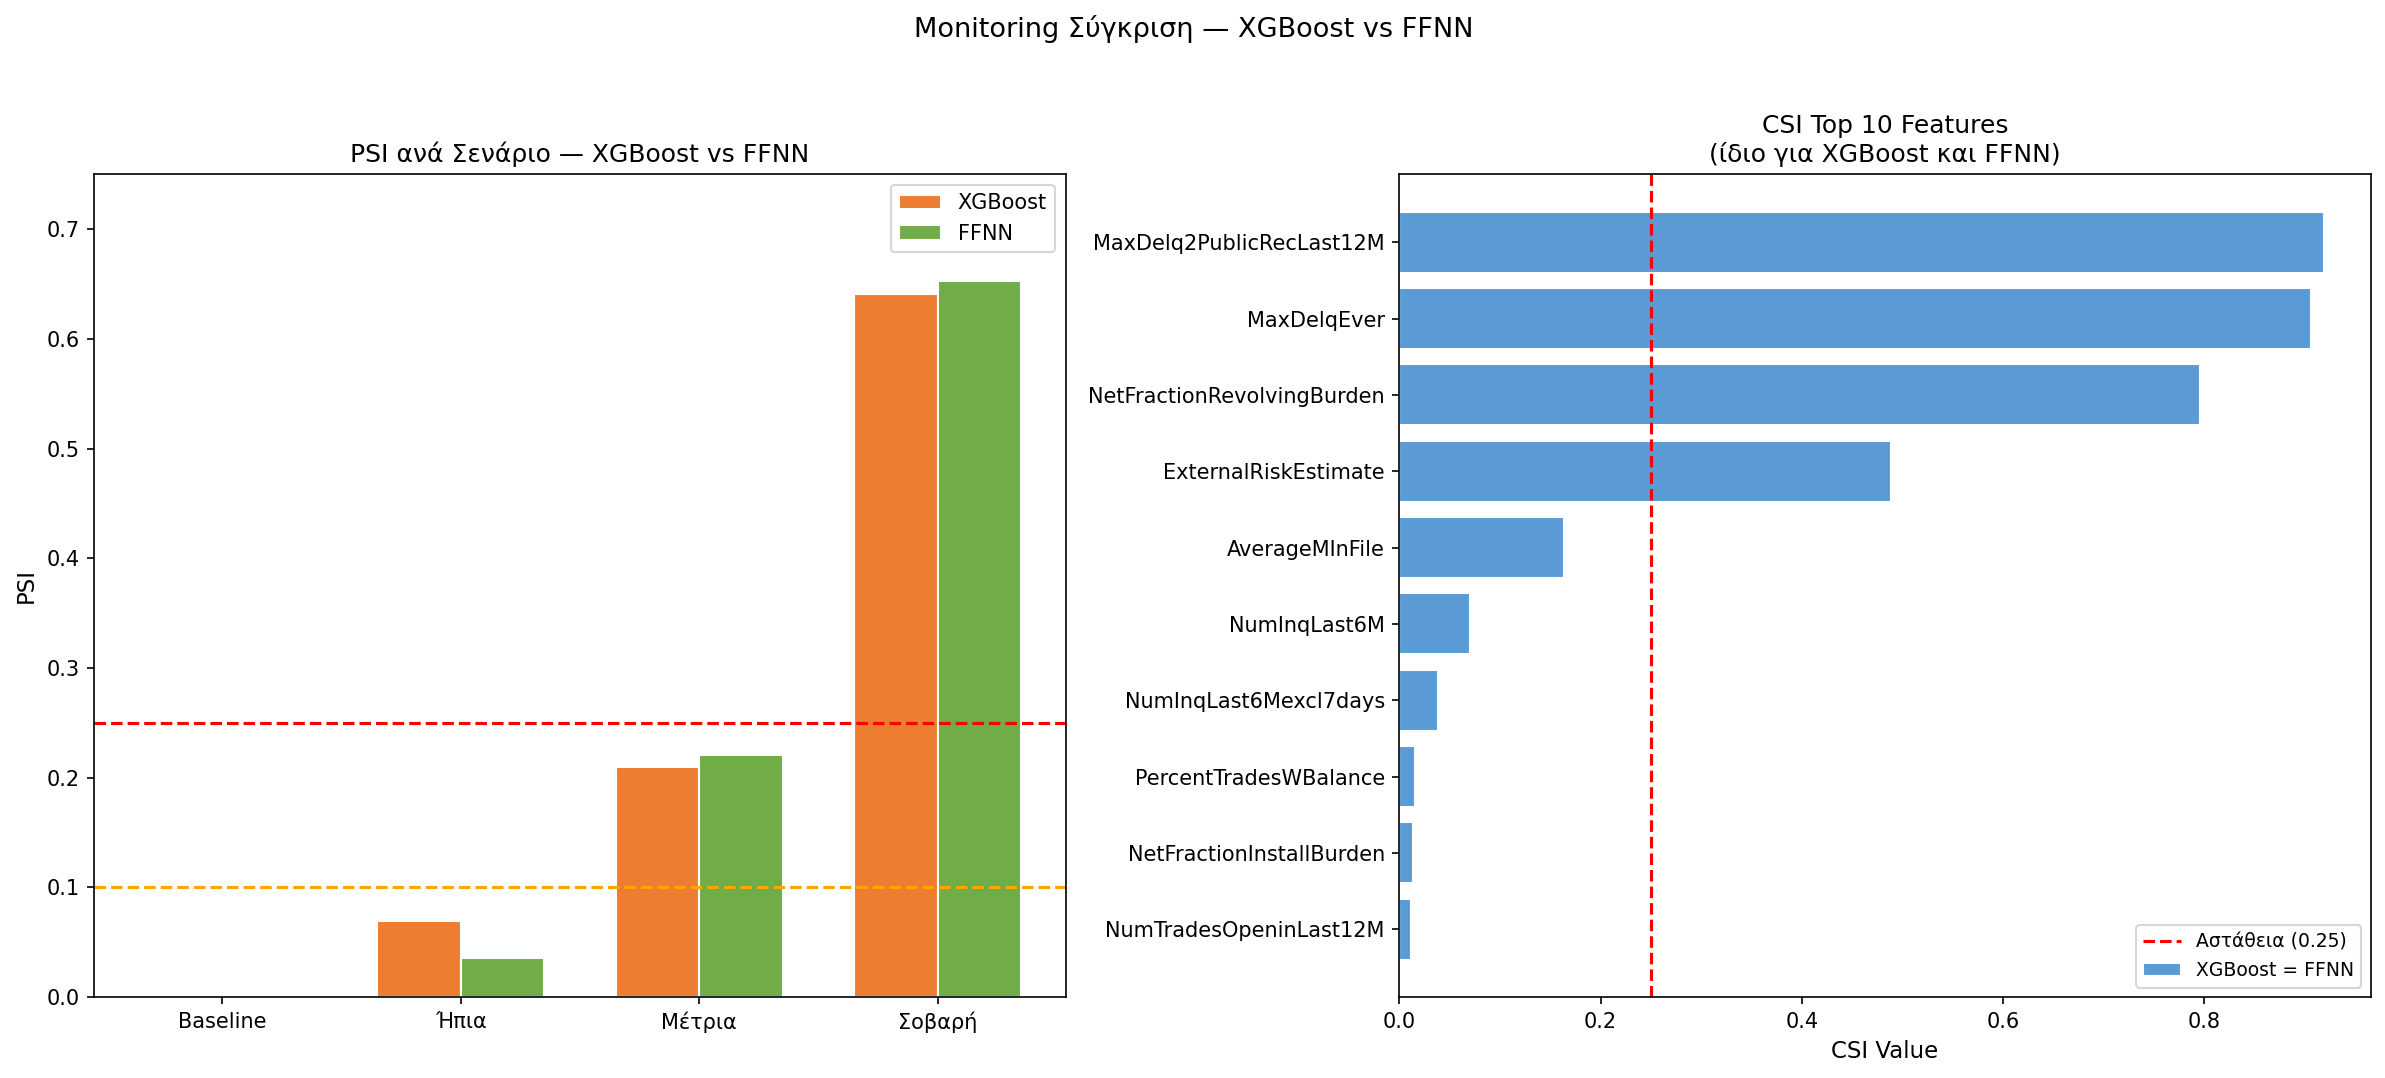
\includegraphics[width=\textwidth]{21_monitoring_comparison}
    \caption[Σύγκριση παρακολούθησης XGBoost vs FFNN]{Σύγκριση παρακολούθησης XGBoost και FFNN. Αριστερά: PSI ανά
             σενάριο οικονομικής επιδείνωσης --- οι τιμές των δύο μοντέλων
             είναι παρόμοιες. Δεξιά: CSI για τα 10 πιο ασταθή
             χαρακτηριστικά --- ταυτόσημο και για τα δύο μοντέλα, καθώς
             εξαρτάται από την είσοδο και όχι από την εσωτερική λογική
             του μοντέλου.}
    \label{fig:monitoring_comparison}
\end{figure}

%==============================================================
\section{Συγκεντρωτική Αξιολόγηση}
\label{sec:results_summary}
% 23_summary_table.png
Τα αποτελέσματα του κεφαλαίου οδηγούν σε τέσσερα κύρια συμπεράσματα
για τα τέσσερα βασικά σημεία της εργασίας. Όσον αφορά την απόδοση,
τα μοντέλα Logistic Regression, XGBoost και FFNN έχουν οριακές διαφορές
με το XGBoost να προηγείται ελαφρώς. Αυτό οφείλεται κυρίως στην
προεπεξεργασία της βάσης δεδομένων και τη γραμμικοποίησή της.
Η ερμηνευσιμότητα είναι το κύριο χαρακτηριστικό που διαφοροποιεί τους
αλγορίθμους XGBoost και FFNN. Ο πρώτος είναι πλήρως ερμηνεύσιμος με
μικρό υπολογιστικό κόστος, ενώ ο δεύτερος απαιτεί δυσανάλογους πόρους,
απαγορευτικούς για χρήση σε μεγάλες βάσεις δεδομένων με πολλά
χαρακτηριστικά. Όσον αφορά τη μεροληψία, και τα τρία μοντέλα εμφάνισαν
καθαρά σημάδια της. Το γεγονός αυτό αποδεικνύει ότι η αιτία ήταν τα
δεδομένα της βάσης. Επιπλέον, καθίσταται σαφές ότι ο μετριασμός της
μεροληψίας κοστίζει στον τομέα της απόδοσης. Τέλος, η παρακολούθηση
των μοντέλων είναι εξίσου εύκολη χωρίς να εξαρτάται από την
πολυπλοκότητά τους, γεγονός που δεν μειώνει τη σημαντικότητα της
ερμηνευσιμότητας, καθώς αυτή συνεχίζει να είναι αναγκαία. Το μοντέλο
XGBoost φαίνεται να είναι η καλύτερη επιλογή στην πρόβλεψη του
πιστωτικού κινδύνου, τόσο λόγω της εύκολης και πλήρους
ερμηνευσιμότητάς του όσο και της ικανότητάς του στην αναγνώριση μη
γραμμικών σχέσεων. Η πρόταση πλαισίου επικύρωσης του
Κεφαλαίου~\ref{ch:framework} είναι απόρροια των παραπάνω συμπερασμάτων.

% -------------------------------------------------------------------
% Σχήμα 4.21 — Summary Table (NB02)
% Τοποθέτηση: αμέσως μετά το κείμενο ανάλυσης
% -------------------------------------------------------------------
\begin{figure}[htbp]
    \centering
    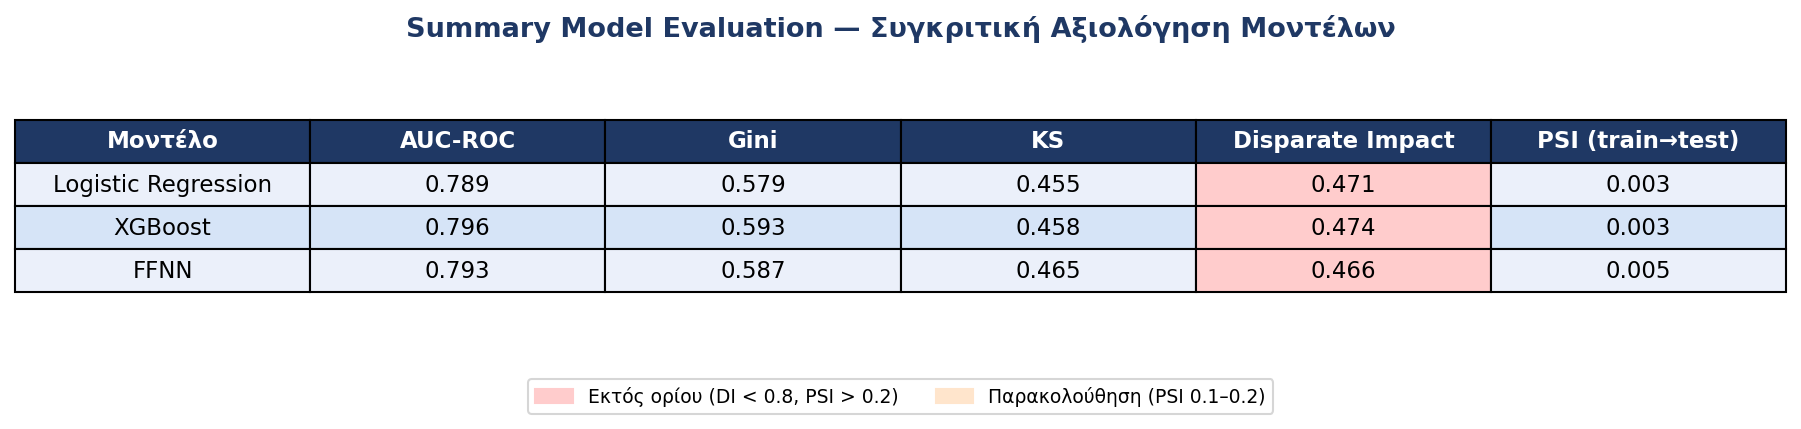
\includegraphics[width=\textwidth]{23_summary_table}
    \caption[Συγκεντρωτικός πίνακας αξιολόγησης μοντέλων]{Συγκεντρωτικός πίνακας αξιολόγησης των τριών μοντέλων.
             Χρωματική κωδικοποίηση: κόκκινο = εκτός ορίου
             (DI $< 0{,}80$, PSI $> 0{,}25$),
             πορτοκαλί = παρακολούθηση (PSI $0{,}10$--$0{,}25$).}
    \label{fig:summary_table}
\end{figure}

   % Πειραματικά Αποτελέσματα
%==============================================================
% ΚΕΦΑΛΑΙΟ 5 — ΠΡΟΤΑΣΗ ΠΛΑΙΣΙΟΥ ΕΠΙΚΥΡΩΣΗΣ
%==============================================================
\chapter{Πρόταση Πλαισίου Επικύρωσης}
\label{ch:framework}

Όσα προηγήθηκαν στην εργασία συνδυάζονται στο παρόν κεφάλαιο για
την δημιουργία και διατύπωση μιας σειράς προτάσεων για ένα πλαίσιο
επικύρωσης μοντέλων μηχανικής μάθησης στον πιστωτικό κίνδυνο.
Τα ευρήματα του Κεφαλαίου~\ref{ch:results} έχουν σημαντικό ρόλο
στη διαμόρφωσή του. Η ενότητα~\ref{sec:principles} αφορά τις
βασικές αρχές σχεδιασμού του πλαισίου. Στην
ενότητα~\ref{sec:workflow} περιγράφεται η πρότυπη ροή εργασιών
επικύρωσης μοντέλων μηχανικής μάθησης. Η
ενότητα~\ref{sec:complexity_requirements} έχει ως κύριο θέμα τις
διαφοροποιήσεις λόγω της πολυπλοκότητας κάθε μοντέλου και τέλος
η ενότητα~\ref{sec:limitations} περιέχει τους περιορισμούς και
τις γενικεύσεις του πλαισίου.

%==============================================================
\section{Αρχές Σχεδιασμού}
\label{sec:principles}
%==============================================================

Για τη δόμηση του πλαισίου επικύρωσης είναι αναγκαία η διαίρεση
του σε βασικές αρχές. Η ανάλυση της θεωρίας στο
Κεφάλαιο~\ref{ch:theory} και τα πειραματικά αποτελέσματα του
Κεφαλαίου~\ref{ch:results} οδηγούν στις ακόλουθες αναγκαίες
αρχές, θεμέλια για το προτεινόμενο πλαίσιο.

\paragraph{Αρχή 1 --- Αναλογικότητα ελέγχου με την πολυπλοκότητα.}
Η εντατικότητα του ελέγχου πρέπει να είναι αναλογική όπου χρειάζεται,
 με βάση εμπειρική ανάλυσης, της
πολυπλοκότητας του μοντέλου. Η παρούσα αρχή ικανοποιεί τις απαιτήσεις των EBA Guidelines και του 
SR Letter~11-7 \citep{eba2023, sr117}, οι οποίες υιοθετούν την αρχή της 
proportionality στο model risk management \citep{bis2024principles}. Η ανάλυση
του μοντέλου FFNN απαίτησε ${\sim}2{,}5$ ώρες για τον υπολογισμό
τιμών SHAP ενώ το XGBoost μερικά δευτερόλεπτα
(βλ.\ ενότητα~\ref{sec:results_ffnn_shap}).

\paragraph{Αρχή 2 --- Η ερμηνευσιμότητα ως μη διαπραγματεύσιμη απαίτηση.}
Για κάθε μοντέλο ανεξαρτήτως πολυπλοκότητας είναι αναγκαία η
ύπαρξη μηχανισμού επεξήγησης των αποτελεσμάτων του σε ατομικό
αλλά και καθολικό επίπεδο. Οι ρυθμιστικές αρχές υποχρεώνουν
την ύπαρξη ανάλογου μηχανισμού για την ικανοποίηση του
«δικαιώματος εξήγησης» \citep{goodman2017european, eba2023} σε πρώτο ή και δεύτερο επίπεδο, όπως
αναφέρθηκε στην ενότητα~\ref{sec:results_pdp}. Η επιλογή
μοντέλου λοιπόν πρέπει να περιορίζεται σε αλγορίθμους οι οποίοι
συνοδεύονται από αξιόπιστο μηχανισμό post-hoc εξήγησης. Από τα
αποτελέσματα της ενότητας~\ref{sec:results_ffnn_shap} φαίνεται
πρακτικά ότι η ύπαρξη ενός τέτοιου μηχανισμού και η αξιοπιστία
του εξαρτάται από την πολυπλοκότητα του μοντέλου, συνδέοντας
τις Αρχές 1 και 2.

\paragraph{Αρχή 3 --- Διαχωρισμός μεροληψίας μοντέλου από μεροληψία δεδομένων.}
Πρέπει να γίνεται έρευνα για ανίχνευση μεροληψίας σε όλα τα
μοντέλα ώστε να γίνεται εμφανής η πηγή της. Μεροληψία μπορεί
να εμφανιστεί λόγω της βάσης δεδομένων
(βλ.\ ενότητα~\ref{subsec:bias_detection}) αλλά να ερμηνευθεί
λανθασμένα ως σφάλμα στην εσωτερική λογική κάποιου μοντέλου.
Για την εμπειρική απόδειξη της πηγής της μεροληψίας είναι
απαραίτητη η σύγκριση των αποτελεσμάτων των μοντέλων. Η
συγκεκριμένη αρχή προσθέτει στη διαδικασία μετριασμού
μεροληψίας, εφόσον δεν στοχεύει μόνο στον μετριασμό της αλλά
και στην αιτία εμφάνισής της.

\paragraph{Αρχή 4 --- Παρακολούθηση ως συνεχής διαδικασία και όχι ως τελικός έλεγχος.}
Η διαδικασία της επικύρωσης πρέπει να είναι μια διαρκής
διαδικασία. Η μεταβολή στα δεδομένα (Data Drift) και στο
μοντέλο (Model Drift) έχει αποδειχθεί από τη βιβλιογραφία ότι
είναι αναπόφευκτη~\citep{widmer1996learning}. Οι αλγόριθμοι
θα πρέπει να παρακολουθούνται περιοδικά με δείκτες όπως ο PSI
και CSI, οι οποίοι όπως απέδειξε η εργασία είναι ικανοί να
παράγουν αξιόπιστες προειδοποιήσεις. Επιτρέπεται έτσι η
διάγνωση και η έγκαιρη επανεκπαίδευση του μοντέλου προς την
αποφυγή αισθητής υποβάθμισης των προβλέψεων.


\paragraph{Αρχή 5 --- Κανονιστική συμμόρφωση ως ελάχιστο, όχι ως στόχος.}
Οι απαραίτητες προς συμμόρφωση απαιτήσεις των Basel~II/III,
SR~11-7 και EBA Guidelines \citep{basel2017, sr117, eba2023} αποτελούν ελάχιστο επίπεδο προς
κάλυψη και όχι όριο. Για τους δείκτες DPD, DI, καθώς και PSI,
CSI, νομοθετούνται όρια των οποίων η ικανοποίηση δεν εγγυάται
την πλήρη ηθική κάλυψη των αποφάσεων του μοντέλου. Είναι
γνωστό από τη βιβλιογραφία ότι η νομική συμμόρφωση δεν
εξαντλεί την ηθική υποχρέωση~\citep{barocas2019fairness, selbst2019fairness},
ακόμη και όταν η ηθική κάλυψη συνεπάγεται απώλεια
προβλεπτικής ικανότητας. Η αρνητική αυτή επίπτωση κοστίζει
στον τραπεζικό τομέα, όμως η απώλεια μπορεί να μετριαστεί
και να διατηρηθεί σε χαμηλά επίπεδα. Στην εργασία φτάνουμε
σε τέλεια βαθμολογία DI $= 1$ με Balanced Accuracy μόλις
$-0{,}022$.

%==============================================================
\section{Βήματα Validation Workflow}
\label{sec:workflow}
%==============================================================

Για τη ροή επικύρωσης προτείνεται διαδικασία επτά βημάτων.
Τα βήματα πρέπει να εφαρμόζονται με τη σειρά που δίνονται.
Συγκεκριμένα βήματα διαφοροποιούνται ανάλογα με την
πολυπλοκότητα του μοντέλου, όπως φαίνεται αναλυτικά στην
ενότητα~\ref{sec:complexity_requirements}.

\paragraph{Βήμα 1 --- Προεπεξεργασία και διαχωρισμός δεδομένων.}
Εάν η βάση περιέχει εγγραφές χωρίς πληροφορία, τότε πρέπει
οι εγγραφές αυτές είτε να διαγράφονται ή να συμπληρώνονται
με εκτιμώμενες τιμές ανάλογα με τη βάση. Κωδικοποίηση
κατηγορικών μεταβλητών ώστε να μπορούν να χρησιμοποιηθούν
από αλγορίθμους μηχανικής μάθησης. Στη συνέχεια ο
διαχωρισμός σε train, validation και test sets πρέπει να
γίνεται με stratification ώστε να εξασφαλίζεται η αναλογία
στις κλάσεις. Τέλος, εάν απαιτείται κανονικοποίηση, αυτή
πρέπει να υλοποιείται με fit μόνο στο training set, ενώ στα
test και validation sets με transform, για να αποφευχθεί
το data leakage.

\paragraph{Βήμα 2 --- Εκπαίδευση μοντέλου και έλεγχος υπερπροσαρμογής.}
Μετά την επιλογή υπερπαραμέτρων (βάθος δέντρου, learning
rate, regularization strength) και την εκπαίδευση με αυτές,
πρέπει να γίνεται άμεσα σύγκριση απόδοσης στα train και
validation sets και έλεγχος υπερπροσαρμογής. Ως ένδειξη
υπερπροσαρμογής μπορεί να χρησιμοποιηθεί η σχετική πτώση
μεγαλύτερη του ${\sim}5\%$ (ad-hoc όριο βασισμένο στα ευρήματα
του Κεφαλαίου~\ref{ch:results}). Σε περίπτωση υπερπροσαρμογής
πρέπει να γίνει επανεξέταση των παραμέτρων ή χρήση τεχνικών
regularization (βλ.\ Πίνακα~\ref{tab:overfitting}). Η
οριακή παραβίαση από μοντέλα δέντρων αποφάσεων μπορεί να
αντιμετωπιστεί με early stopping και stochastic
regularization, οπότε επιτρέπεται μικρή ανοχή για την
περίπτωση αυτή.

\paragraph{Βήμα 3 --- Αξιολόγηση απόδοσης σε πολλαπλούς άξονες.}
Υπολογισμός των μετρικών AUC-ROC, Gini και KS στο test set,
καθώς και ανάλυση πίνακα σύγχυσης, καμπυλών Precision/Recall
ως προς το threshold, ανάλυση κατά δεκατημόρια και
διαγραμμάτων βαθμονόμησης. Κάθε μετρική είναι απαραίτητη
και συμπληρώνει την εικόνα για τη λειτουργία του μοντέλου.
Επιπλέον είναι αναγκαίες για τη συμμόρφωση με τις εποπτικές
αρχές~\citep{basel2017, sr117, eba2023}.

\paragraph{Βήμα 4 --- Ερμηνεία αποφάσεων.}
Ερμηνεία αποφάσεων μοντέλου μέσω SHAP feature importance και
beeswarm διαγραμμάτων για καθολική σημαντικότητα μεταβλητών,
καθώς και SHAP waterfall plots και Partial Dependence Plots
για ατομική σημαντικότητα χαρακτηριστικών ανά
μοντέλο~\citep{lundberg2017shap}. Για μοντέλα δέντρων
αποφάσεων είναι προτιμότερη η συνάρτηση TreeExplainer
(ακριβής, υπολογιστικά αποδοτική), ενώ για νευρωνικά δίκτυα
η KernelExplainer, η οποία όμως επιφέρει σημαντικό
υπολογιστικό κόστος.

\paragraph{Βήμα 5 --- Ανίχνευση μεροληψίας σε όλα τα μοντέλα.}
Αρχικά πρέπει να γίνει επιλογή ευαίσθητου χαρακτηριστικού
και διαχωρισμός των δεδομένων σε ομάδες βάσει αυτού.
Υπολογισμός DPD και DI με τη βιβλιοθήκη
Fairlearn~\citep{bird2020fairlearn} σε πολλαπλά μοντέλα,
ώστε σε πιθανή σύγκλιση αποτελεσμάτων να εντοπιστεί ότι η
βάση αποτελεί την πηγή μεροληψίας.

\paragraph{Βήμα 6 --- Μετριασμός μεροληψίας με αξιολόγηση κόστους.}
Εφόσον εντοπιστεί μεροληψία, εφαρμόζεται τεχνική μετριασμού
(in-processing για Logistic Regression, post-processing για
XGBoost). Η τεχνική μετριασμού θα επιφέρει κόστος στην
απόδοση, το οποίο πρέπει να καταγραφεί. Στην εργασία κατά
το post-processing (ThresholdOptimizer) διατηρείται το AUC
σταθερό αλλά μειώνεται το Balanced Accuracy, ενώ κατά το
in-processing (\texttt{ExponentiatedGradient}) μειώνεται η
AUC κατά ${\sim}14\%$. Η εξισορρόπηση ανάμεσα στην
αξιοπιστία πρόβλεψης έναντι της ισορροπίας ομάδων
εξαρτάται από τους ισχύοντες νόμους, την ηθική πυξίδα και
τις επιχειρηματικές προτεραιότητες της τράπεζας.

\paragraph{Βήμα 7 --- Συνεχής παρακολούθηση μετά το deployment.}
Συνεχής υπολογισμός PSI και CSI για πιθανή αλλαγή στα
δεδομένα εισόδου και τις προβλέψεις των
αλγορίθμων~\citep{eba2023}. Συγκεκριμένα, τιμές κάτω του
$0{,}10$ δηλώνουν σταθερότητα, μεταξύ $0{,}10$ και $0{,}25$
απαιτούν αυξημένη παρακολούθηση και άνω του $0{,}25$
επιβάλλουν επανεκπαίδευση. Σε περιπτώσεις αστάθειας
απαιτείται ανάλυση SHAP για τον εντοπισμό των
χαρακτηριστικών που την προκάλεσαν. Όπως αναφέρθηκε στο
Βήμα~4, το υπολογιστικό κόστος της ανάλυσης διαφέρει
σημαντικά ανά μοντέλο και πρέπει να ληφθεί υπόψη εκ των
προτέρων.

%==============================================================
\section{Απαιτήσεις Επικύρωσης ανά Επίπεδο Πολυπλοκότητας}
\label{sec:complexity_requirements}
%==============================================================

Οι παρακάτω Πίνακες~\ref{tab:complexity_a} και~\ref{tab:complexity_b}
παρουσιάζουν τις διαφορές στις απαιτήσεις επικύρωσης για τα τρία
μοντέλα της εργασίας. Μέσω των αποτελεσμάτων που παρουσιάζονται
γίνεται σαφής η διαφοροποίηση στο πλαίσιο επικύρωσης ανάλογα με
την πολυπλοκότητα του αλγορίθμου.

\begin{table}[htbp]
    \centering
    \renewcommand{\arraystretch}{1.3}
    \caption[Απαιτήσεις επικύρωσης ανά πολυπλοκότητα — Ερμηνευσιμότητα \& Απόδοση]{Διαφοροποιημένες απαιτήσεις επικύρωσης ανά επίπεδο
             πολυπλοκότητας --- Ερμηνευσιμότητα \& Απόδοση.
             Οι τιμές προέρχονται από τα ευρήματα του
             Κεφαλαίου~\ref{ch:results}.}
    \label{tab:complexity_a}
    \small
    \begin{tabular}{p{3.8cm}p{3.8cm}p{3.8cm}}
        \toprule
        \textbf{Απαίτηση} &
        \textbf{Logistic Regression} &
        \textbf{XGBoost} \\
        \midrule
        Εγγενής ερμηνευσιμότητα &
        Πλήρης (συντελεστές $\beta$) &
        Καμία \\
        \midrule
        Post-hoc εξήγηση &
        Δεν απαιτείται &
        SHAP TreeExplainer (δευτερόλεπτα) \\
        \midrule
        Έλεγχος υπερπροσαρμογής &
        Σχεδόν περιττός (1{,}3\%) &
        Κρίσιμος (6{,}2\%) \\
        \midrule
        Αξιοπιστία βαθμονόμησης &
        Υψηλή (log-loss training) &
        Μέτρια (απόκλιση στις άκρες) \\
        \bottomrule
    \end{tabular}

    \vspace{0.4cm}

    \begin{tabular}{p{3.8cm}p{3.8cm}p{3.8cm}}
        \toprule
        \textbf{Απαίτηση} &
        \textbf{XGBoost} &
        \textbf{FFNN} \\
        \midrule
        Εγγενής ερμηνευσιμότητα &
        Καμία &
        Καμία \\
        \midrule
        Post-hoc εξήγηση &
        SHAP TreeExplainer (δευτερόλεπτα) &
        SHAP KernelExplainer (${\sim}2{,}5$ ώρες) \\
        \midrule
        Έλεγχος υπερπροσαρμογής &
        Κρίσιμος (6{,}2\%) &
        Μέτριος (2{,}6\%) \\
        \midrule
        Αξιοπιστία βαθμονόμησης &
        Μέτρια (απόκλιση στις άκρες) &
        Χαμηλή (ακανόνιστη) \\
        \bottomrule
    \end{tabular}
\end{table}

\begin{table}[htbp]
    \centering
    \renewcommand{\arraystretch}{1.3}
    \caption[Απαιτήσεις επικύρωσης ανά πολυπλοκότητα — Δικαιοσύνη \& Παρακολούθηση]{Διαφοροποιημένες απαιτήσεις επικύρωσης ανά επίπεδο
             πολυπλοκότητας --- Δικαιοσύνη \& Παρακολούθηση.
             Οι τιμές προέρχονται από τα ευρήματα του
             Κεφαλαίου~\ref{ch:results}.}
    \label{tab:complexity_b}
    \small
    \begin{tabular}{p{3.8cm}p{3.8cm}p{3.8cm}}
        \toprule
        \textbf{Απαίτηση} &
        \textbf{Logistic Regression} &
        \textbf{XGBoost} \\
        \midrule
        Τεχνική μετριασμού bias &
        In-processing (\texttt{Exp.\ Gradient}) &
        Post-processing (Thresh.\ Opt.) \\
        \midrule
        Κόστος μετριασμού bias &
        AUC: $-14\%$ &
        AUC: $0\%$ / Bal.\ Acc.: $\downarrow$ \\
        \midrule
        Παρακολούθηση (PSI/CSI) &
        Τυπική &
        Τυπική \\
        \midrule
        Σύνδεση drift με χαρακτηριστικά &
        Άμεση (συντελεστές) &
        Γρήγορη (TreeExplainer) \\
        \midrule
        Συνολικό κόστος επικύρωσης &
        Χαμηλό &
        Μέτριο \\
        \bottomrule
    \end{tabular}

    \vspace{0.4cm}

    \begin{tabular}{p{3.8cm}p{3.8cm}p{3.8cm}}
        \toprule
        \textbf{Απαίτηση} &
        \textbf{XGBoost} &
        \textbf{FFNN} \\
        \midrule
        Τεχνική μετριασμού bias &
        Post-processing (Thresh.\ Opt.) &
        Δεν εξετάστηκε \\
        \midrule
        Κόστος μετριασμού bias &
        AUC: $0\%$ / Bal.\ Acc.: $\downarrow$ &
        --- \\
        \midrule
        Παρακολούθηση (PSI/CSI) &
        Τυπική &
        Τυπική (CSI ταυτόσημο) \\
        \midrule
        Σύνδεση drift με χαρακτηριστικά &
        Γρήγορη (TreeExplainer) &
        Πρακτικά απαγορευτική (KernelExplainer) \\
        \midrule
        Συνολικό κόστος επικύρωσης &
        Μέτριο &
        Πολύ υψηλό \\
        \bottomrule
    \end{tabular}
\end{table}


Τα κύρια συμπεράσματα είναι τρία. Αρχικά, οι απαιτήσεις επικύρωσης
δεν αυξάνονται γραμμικά όσο αυξάνεται η πολυπλοκότητα αλλά
δυσανάλογα περισσότερο. Πιο συγκεκριμένα, η διαφορά ανάμεσα στις
απαιτήσεις για το μοντέλο XGBoost και την Logistic Regression είναι
σημαντικά μικρότερη από τη διαφορά XGBoost και FFNN. Ταυτόχρονα η
τελευταία αύξηση στην πολυπλοκότητα από XGBoost σε FFNN δεν εισάγει
ουσιαστικό πλεονέκτημα στην απόδοση του αλγορίθμου. Δεύτερον, οι
απαιτήσεις παρακολούθησης του μοντέλου παραμένουν σταθερές, αλλά η
ανάγκη ερμηνείας τους εμφανίζει διαφοροποίηση στο κόστος υπολογισμού.
Η παρακολούθηση μοντέλου χρησιμοποιεί τις μετρικές PSI και CSI που
υπολογίζουν διαφορές στα δεδομένα που εισάγονται στα μοντέλα, άρα ο
υπολογισμός τους δεν διαφέρει ανά μοντέλο. Σε περίπτωση όμως
διαπίστωσης σημαντικής αλλαγής στα δεδομένα εισαγωγής είναι αναγκαία
η ερμηνεία τους μέσω SHAP που διαφέρει ανά μοντέλο. Συμπεραίνεται
έτσι ότι η απόδοση δεν είναι το μοναδικό κριτήριο για την επιλογή
του μοντέλου, καθώς η επικύρωση και η συνεχής παρακολούθησή του,
οι οποίες είναι αναγκαίες, αποτελούν παράγοντες βιωσιμότητάς του.

Με βάση τα παραπάνω, για τη συγκεκριμένη βάση το μοντέλο XGBoost
κρίνεται ως το καταλληλότερο από τα τρία μοντέλα. Η προβλεπτική
ικανότητά του υπερέχει έστω και ελαφρά έναντι των άλλων μοντέλων,
ενώ το κόστος ερμηνείας του παραμένει σε αποδεκτά όρια. Επιπλέον,
επιτρέπει τον μετριασμό μεροληψίας post-processing, ο οποίος δεν
εμφανίζει απώλειες στον δείκτη AUC, με μόλις $-0{,}022$ στο
Balanced Accuracy, και δεν απαιτεί επανεκπαίδευση μοντέλου. Το
μοντέλο FFNN εμφανίζει καλύτερη απόδοση έναντι του XGBoost μόνο
στον δείκτη KS ($0{,}465$ έναντι $0{,}458$) με αποτέλεσμα να μην
δικαιολογείται το δυσανάλογο κόστος ερμηνείας του.

%==============================================================
\section{Περιορισμοί και Γενικευσιμότητα}
\label{sec:limitations}
%==============================================================

Το πλαίσιο που προτείνεται, παρότι προκύπτει από τα αποτελέσματα
και το κανονιστικό πλαίσιο, χαρακτηρίζεται από περιορισμούς.
Η ανάλυση αυτών των περιορισμών κρίνεται αναγκαία, καθώς
επηρεάζεται άμεσα η γενικευσιμότητα των πορισμάτων.

\paragraph{Ένα μόνο dataset.}
Στην παρούσα εργασία χρησιμοποιείται μόνο μια βάση δεδομένων,
η FICO HELOC. Η συγκεκριμένη βάση έχει μερικές ιδιαιτερότητες.
Αρχικά, περιέχει συγκεντρωτικά χαρακτηριστικά όπως το
\texttt{ExternalRiskEstimate}. Τα συγκεκριμένα χαρακτηριστικά
εμφανίζουν σχετικά μονότονη συμπεριφορά σε σχέση με τον
πιστωτικό κίνδυνο, με αποτέλεσμα η διαφορά στην απόδοση μεταξύ
της Logistic Regression --- η οποία δεν αναγνωρίζει μη γραμμικές
σχέσεις ανάμεσα στα χαρακτηριστικά και την τελική πρόβλεψη ---
και πιο σύνθετων μοντέλων να μειώνεται. Σε βάσεις δεδομένων με
μη γραμμικά χαρακτηριστικά η διαφορά απόδοσης ενδέχεται να είναι
σημαντικότερη. Επιπλέον, η βάση δεν περιέχει δημογραφικά στοιχεία.
Η απουσία τους οδήγησε στον ορισμό proxy μεταβλητής, και
συγκεκριμένα της \texttt{AverageMInFile}. Η μεταβλητή
\texttt{AverageMInFile} δεν αποτελεί προστατευόμενο χαρακτηριστικό
αλλά είναι feature κινδύνου. Λόγω αυτού, η μείωση στην απόδοση
λόγω της διαδικασίας εξάλειψης της μεροληψίας ενδέχεται να είναι
τεχνικά αυξημένη. Η επιλογή proxy μεταβλητής είναι θεμιτή ως προς
την επίδειξη της μεθοδολογίας, αλλά δεν αντικαθιστά πλήρως την
ανάλυση σε πραγματικές προστατευόμενες μεταβλητές. Συνεπώς, σε
βάσεις δεδομένων όπου η εξάλειψη μεροληψίας γίνεται σε
προστατευόμενα χαρακτηριστικά, αναμένεται η απώλεια απόδοσης
λόγω mitigation να είναι μικρότερη.

\paragraph{Στατική προσομοίωση μετατόπισης δεδομένων.}
Η διαδικασία παρακολούθησης των μοντέλων βασίστηκε σε τρία
σενάρια οικονομικής επιδείνωσης (ήπια, μέτρια, σοβαρή) τα οποία
παράχθηκαν τεχνικά με τη χρήση Γκαουσιανού θορύβου. Η προσέγγιση
αυτή, ενώ είναι κατάλληλη για επίδειξη χρήσης των δεικτών PSI και
CSI, δεν περιέχει ακριβή στοιχεία οικονομικής κρίσης. Κατά την
περίοδο μιας οικονομικής κρίσης αναμένεται να εμφανίσουν
συσχετισμένες μετατοπίσεις πολλαπλά χαρακτηριστικά, σε αντίθεση
με την προσομοίωση που εμφάνισαν μόνο τρία, ενώ στα υπόλοιπα
είχε προστεθεί απλά λευκός θόρυβος.

\paragraph{Εστίαση στην πιθανότητα αθέτησης.}
Στον τραπεζικό τομέα, για τη συνολική διαχείριση ενός
χαρτοφυλακίου είναι αναγκαία η πρόβλεψη της Ζημίας σε Περίπτωση
Αθέτησης (LGD) και της Έκθεσης σε Περίπτωση Αθέτησης (EAD),
εκτός από την Πιθανότητα Αθέτησης (PD)~\citep{mcneil2015}. Το
πλαίσιο που προτείνεται στην εργασία δεν επεκτείνεται στην
πρόβλεψη των δύο πρώτων μεταβλητών, καθώς υπερβαίνει τον σκοπό
της. Ως αποτέλεσμα, το παρόν πλαίσιο δεν αποτελεί ολοκληρωμένη
πρόταση για τη διαχείριση χαρτοφυλακίου, αλλά μόνο για την
πρόβλεψη της πιθανότητας αθέτησης.

\paragraph{Επιλογή υπερπαραμέτρων.}
Δεν έγινε βελτιστοποίηση υπερπαραμέτρων πριν από την εκπαίδευση
των μοντέλων για την επίτευξη βέλτιστης απόδοσης. Στην παρούσα
εργασία τα τρία μοντέλα εκπαιδεύτηκαν με λογικές αρχικές τιμές,
οι οποίες όμως δεν παράγουν τη βέλτιστη δυνατή απόδοση των
μοντέλων. Η επιλογή αυτή έγινε διότι, μέσω της βελτιστοποίησης
υπερπαραμέτρων, ενώ ενδέχεται να υπάρξουν ελαφρές βελτιώσεις
στην απόδοση των μοντέλων, δεν επηρεάζονται οι απαιτήσεις
ερμηνείας και παρακολούθησης. Έτσι, η εξαντλητική χρήση της
αποτελεί επιλογή για εργασίες με κεντρικό ζήτημα τη
μεγιστοποίηση της απόδοσης κάθε μοντέλου.

\paragraph{Γενικευσιμότητα του πλαισίου.}
Παρά τους περιορισμούς που αναφέρθηκαν, η δομή του πλαισίου που
προτείνεται παραμένει εφαρμόσιμη. Οι αρχές σχεδιασμού, η πρότυπη
ροή εργασιών και οι κλιμακούμενες απαιτήσεις ανά πολυπλοκότητα
επεκτείνονται σε προβλήματα πρόβλεψης PD σε όλα τα είδη δανείων,
σε υλοποιήσεις άλλων συγγενικών αλγορίθμων (LightGBM, CatBoost),
αλλά και σε άλλα binary classification προβλήματα του
χρηματοπιστωτικού τομέα (ανίχνευση απάτης, prepayment risk). Η
βασική ιδέα επικύρωσης και ερμηνευσιμότητας αναλογικά με την
πολυπλοκότητα παραμένει αναλλοίωτη, ανεξαρτήτως βάσης δεδομένων
και αλγορίθμων. Έτσι, αποτελεί σαφή απάντηση στο ερώτημα της
εργασίας.   % Πρόταση Πλαισίου Επικύρωσης
%==============================================================
% ΚΕΦΑΛΑΙΟ 6 — ΣΥΜΠΕΡΑΣΜΑΤΑ ΚΑΙ ΜΕΛΛΟΝΤΙΚΕΣ ΕΠΕΚΤΑΣΕΙΣ
%==============================================================
\chapter{Συμπεράσματα και Μελλοντικές Επεκτάσεις}
\label{ch:conclusions}

Η παρούσα εργασία εξέτασε την επικύρωση, ερμηνεία και παρακολούθηση
μοντέλων μηχανικής μάθησης στον πιστωτικό κίνδυνο, με έμφαση στο πώς
μεταβάλλονται οι απαιτήσεις αυτές καθώς αυξάνεται η πολυπλοκότητα του
μοντέλου. Στο παρόν κεφάλαιο συνοψίζονται τα ευρήματα και διατυπώνονται
οι προτεινόμενες κατευθύνσεις για περαιτέρω έρευνα.

%==============================================================
\section{Σύνοψη της Εργασίας}
\label{sec:summary}
%==============================================================

Η εργασία ξεκίνησε με ανασκόπηση του θεωρητικού και κανονιστικού
πλαισίου του πιστωτικού κινδύνου (Κεφάλαιο~\ref{ch:theory}) και
συνέχισε με συστηματική σύγκριση τριών μοντέλων στη βάση FICO HELOC
(Κεφάλαια~\ref{ch:methodology} και~\ref{ch:results}): ενός Logistic
Regression ως παραδοσιακού σημείου αναφοράς, ενός XGBoost ως κύριου
μοντέλου ανάλυσης και ενός Feed-Forward Neural Network ως
επιδεικτικού benchmark πολυπλοκότητας. Η αξιολόγηση πραγματοποιήθηκε
σε τέσσερις άξονες ---απόδοση, ερμηνευσιμότητα, μεροληψία και
παρακολούθηση--- και τα ευρήματα συντέθηκαν σε μια συγκεκριμένη
πρόταση πλαισίου επικύρωσης (Κεφάλαιο~\ref{ch:framework}).

%==============================================================
\section{Απάντηση στο Κεντρικό Ερευνητικό Ερώτημα}
\label{sec:research_question}
%==============================================================

Το κεντρικό ερώτημα της εργασίας ήταν πώς επικυρώνονται, ερμηνεύονται
και παρακολουθούνται τα μοντέλα μηχανικής μάθησης στον πιστωτικό
κίνδυνο και πώς μεταβάλλονται οι απαιτήσεις όταν αυξάνεται η
πολυπλοκότητα του μοντέλου. Η απάντηση που προκύπτει είναι ότι η
αύξηση της πολυπλοκότητας δεν συνεπάγεται γραμμική αύξηση των
απαιτήσεων επικύρωσης. Ορισμένα στάδια ---όπως η παρακολούθηση
σταθερότητας μέσω PSI και CSI ή η ανίχνευση μεροληψίας μέσω DPD και
DI--- παραμένουν ουσιαστικά αμετάβλητα ανεξάρτητα από το μοντέλο.
Αντίθετα, η ερμηνευσιμότητα είναι ο άξονας στον οποίο η πολυπλοκότητα
έχει δραματική επίπτωση: η μετάβαση από τη γραμμικότητα της
Logistic Regression στη μη γραμμική δομή του XGBoost εισάγει μέτριο
επιπλέον κόστος μέσω του TreeExplainer, ενώ η περαιτέρω μετάβαση στο
FFNN πολλαπλασιάζει το κόστος αυτό κατά τάξεις μεγέθους χωρίς
αντίστοιχο όφελος στην απόδοση. Η ορθή απάντηση στο ερώτημα
επικύρωσης ενός σύνθετου μοντέλου δεν είναι λοιπόν μια ομοιόμορφη
κλιμάκωση όλων των ελέγχων, αλλά μια στοχευμένη ενίσχυση στους
άξονες όπου η πολυπλοκότητα προκαλεί πραγματική απώλεια διαφάνειας.

%==============================================================
\section{Κύρια Συμπεράσματα}
\label{sec:main_conclusions}
%==============================================================

Από τη συστηματική ανάλυση των τεσσάρων αξόνων αξιολόγησης προκύπτουν
τέσσερα κύρια συμπεράσματα.

\paragraph{Απόδοση.}
Τα τρία μοντέλα παρουσίασαν οριακές διαφορές στους δείκτες AUC, Gini
και KS, με το XGBoost να προηγείται ελαφρώς. Το εύρημα αυτό
οφείλεται κυρίως στην εκτεταμένη προεπεξεργασία των χαρακτηριστικών
από την FICO, η οποία γραμμικοποιεί τις σχέσεις μεταξύ τους και
περιορίζει το performance gap. Συνεπάγεται ότι η επιλογή μοντέλου
στον πιστωτικό κίνδυνο δεν μπορεί να γίνεται αποκλειστικά με κριτήριο
την απόδοση, καθώς αυτή ενδέχεται να είναι παρόμοια μεταξύ μοντέλων
διαφορετικής πολυπλοκότητας.

\paragraph{Ερμηνευσιμότητα.}
Ο άξονας αυτός αποτελεί το βασικό σημείο διαφοροποίησης μεταξύ των
μοντέλων. Το XGBoost, μέσω του TreeExplainer, παρέχει ολοκληρωμένη
SHAP ανάλυση σε δευτερόλεπτα, ικανοποιώντας πλήρως το κανονιστικό
«δικαίωμα εξήγησης». Αντίθετα, το FFNN απαιτεί KernelExplainer με
υπολογιστικό κόστος της τάξης των ωρών, καθιστώντας την ερμηνεία
πρακτικά απαγορευτική σε παραγωγικά περιβάλλοντα με μεγάλο όγκο
δεδομένων. Το γεγονός αυτό αποτελεί ισχυρό επιχείρημα κατά της
χρήσης βαθιών νευρωνικών δικτύων στον πιστωτικό κίνδυνο όταν δεν
υπάρχει αντίστοιχο όφελος απόδοσης.

\paragraph{Μεροληψία.}
Και τα τρία μοντέλα εμφάνισαν σχεδόν ταυτόσημες τιμές DPD
(${\sim}0{,}33$) και DI (${\sim}0{,}47$), σαφώς εκτός των αποδεκτών
ορίων. Η σύμπτωση αυτή αποδεικνύει ότι η πηγή της μεροληψίας ήταν τα
δεδομένα και όχι η εσωτερική λογική κάποιου μοντέλου. Επιπλέον, ο
μετριασμός μεροληψίας δεν είναι δωρεάν: η in-processing προσέγγιση
στη Logistic Regression κόστισε ${\sim}14\%$ της AUC, ενώ η
post-processing προσέγγιση στο XGBoost διατήρησε την AUC αλλά
μείωσε το Balanced Accuracy. Η επιλογή τεχνικής μετριασμού αποτελεί
επιχειρηματική απόφαση και πρέπει να γίνεται με ρητή αξιολόγηση του
σχετικού κόστους.

\paragraph{Παρακολούθηση.}
Οι δείκτες PSI και CSI λειτούργησαν αξιόπιστα ως σύστημα έγκαιρης
προειδοποίησης. Στα τρία σενάρια οικονομικής επιδείνωσης, ο PSI
παρήγαγε σταδιακά αυξανόμενες τιμές
($0{,}069 \to 0{,}210 \to 0{,}641$ για το XGBoost), επιτρέποντας
παρέμβαση πριν η απόδοση υποβαθμιστεί. Σημαντικό εύρημα αποτελεί ότι
η ίδια η παρακολούθηση είναι ανεξάρτητη της πολυπλοκότητας του
μοντέλου, καθώς οι δείκτες αυτοί υπολογίζονται επί των δεδομένων ή
των προβλέψεων χωρίς να εξαρτώνται από την εσωτερική δομή του
αλγορίθμου. Η κρίσιμη διαφορά εμφανίζεται κατά τη \emph{διάγνωση}
ενός drift event: εδώ το χαμηλό κόστος ερμηνείας του XGBoost γίνεται
αποφασιστικό πλεονέκτημα έναντι του FFNN.

Συνολικά, τα τέσσερα συμπεράσματα ενισχύουν την κεντρική θέση της
εργασίας ότι το XGBoost αποτελεί τη βέλτιστη επιλογή στο σημερινό
πλαίσιο του πιστωτικού κινδύνου, καθώς συνδυάζει επαρκή απόδοση,
αποδοτική ερμηνευσιμότητα και ευελιξία στον μετριασμό μεροληψίας
χωρίς τις απαγορευτικές απαιτήσεις των βαθιών νευρωνικών δικτύων.

%==============================================================
\section{Μελλοντικές Επεκτάσεις}
\label{sec:future_work}
%==============================================================

Οι περιορισμοί που αναγνωρίστηκαν στην ενότητα~\ref{sec:limitations}
ορίζουν φυσικές κατευθύνσεις για περαιτέρω έρευνα.

\paragraph{Επέκταση σε πολλαπλά datasets.}
Η εφαρμογή του προτεινόμενου πλαισίου σε διαφορετικές βάσεις
δεδομένων ---όπως τα Lending Club, German Credit ή ευρωπαϊκά datasets
καταναλωτικής πίστης--- θα επέτρεπε αξιόπιστο έλεγχο της
γενικευσιμότητας. Datasets χωρίς εκτεταμένη προεπεξεργασία
χαρακτηριστικών αναμένεται να εμφανίσουν μεγαλύτερο performance gap
μεταξύ των μοντέλων, μετατοπίζοντας πιθανώς την ισορροπία μεταξύ
απόδοσης και ερμηνευσιμότητας.

\paragraph{Ανάλυση μεροληψίας σε πραγματικά δημογραφικά χαρακτηριστικά.}
Η χρήση της \texttt{AverageMInFile} ως proxy αποτελεί μεθοδολογική
αναγκαιότητα λόγω της φύσης του HELOC. Η εφαρμογή του πλαισίου σε
βάσεις με πραγματικά δεδομένα φύλου, ηλικίας ή εθνικότητας θα
παρείχε ουσιαστικότερη επικύρωση των μηχανισμών ανίχνευσης και
μετριασμού, σε άμεση συμφωνία με τις απαιτήσεις των ρυθμιστικών
αρχών.

\paragraph{Δυναμική παρακολούθηση με χρονικές σειρές.}
Η αντικατάσταση της στατικής προσομοίωσης drift από πραγματικά
χρονικά δεδομένα θα επέτρεπε τη μελέτη συσχετισμένων μετατοπίσεων σε
πολλαπλά χαρακτηριστικά ταυτόχρονα και τη βαθμονόμηση των ορίων PSI
και CSI σε πραγματικές οικονομικές συνθήκες. Πιθανές πηγές δεδομένων
αποτελούν χρηματοοικονομικές βάσεις που καλύπτουν περιόδους κρίσης
(όπως 2008--2009 ή 2020).

\paragraph{Επέκταση σε LGD και EAD.}
Η παρούσα εργασία επικεντρώθηκε στην πρόβλεψη της PD. Η αντίστοιχη
ανάλυση των παραμέτρων LGD και EAD ---οι οποίες ολοκληρώνουν τον
υπολογισμό της Αναμενόμενης Ζημίας κατά Basel III--- θα προσέφερε
πληρέστερο πλαίσιο επικύρωσης για ολόκληρο τον κύκλο διαχείρισης
του πιστωτικού κινδύνου.

\paragraph{Σύγκριση εναλλακτικών αλγορίθμων Gradient Boosting.}
Η αντιπαραβολή του XGBoost με τις υλοποιήσεις LightGBM και CatBoost
στο ίδιο πλαίσιο θα μπορούσε να αναδείξει αν η υπεροχή του XGBoost
στις απαιτήσεις επικύρωσης διατηρείται ή αν κάποια από τις
εναλλακτικές προσφέρει καλύτερη ισορροπία ταχύτητας, ακρίβειας και
ερμηνευσιμότητας. Παρόμοια συγκριτική ανάλυση θα μπορούσε να γίνει
και μεταξύ των explainers (TreeExplainer, KernelExplainer,
DeepExplainer) ως προς το trade-off ακρίβειας έναντι υπολογιστικού
κόστους.

\paragraph{Αυτοματοποιημένα συστήματα ειδοποίησης.}
Τέλος, η ενσωμάτωση των δεικτών παρακολούθησης σε μηχανισμούς
αυτόματης ειδοποίησης ---με προκαθορισμένα κατώφλια και αυτοματοποιημένη
επανεκπαίδευση--- αποτελεί φυσική συνέχεια του πλαισίου προς ένα
ολοκληρωμένο MLOps περιβάλλον για τον πιστωτικό κίνδυνο, σε ευθεία
συμφωνία με τη φιλοσοφία της συνεχούς επικύρωσης που προβλέπεται
από τις EBA Guidelines.   % Συμπεράσματα

%--------------------------------------------------------------
% BIBLIOGRAPHY
%--------------------------------------------------------------
\cleardoublepage
\bibliography{references/bibliography}

%--------------------------------------------------------------
% APPENDICES (optional)
%--------------------------------------------------------------
% \appendix
% \input{chapters/appendix_a}
% \input{chapters/appendix_b}

\end{document}